\documentclass[12pt,twoside]{report}
\usepackage[a4paper,width=150mm,top=25mm,bottom=25mm]{geometry}
\usepackage[utf8]{inputenc}
\usepackage{graphicx}\graphicspath{ {images/} }
\usepackage{verbatim}
\usepackage{etoolbox}
\usepackage{tabularx}
\usepackage[hyphens]{url}
\urlstyle{same}
\usepackage{amsmath,amssymb}
\usepackage{amsfonts}
\usepackage{hyperref}
 % \usepackage{dsfont}
\usepackage{rotating}
\usepackage{dcolumn}
\usepackage[export]{adjustbox}
\usepackage{fancyhdr}
\usepackage{csquotes}
\usepackage{multicol}
\usepackage{lipsum}
\usepackage{float}
\usepackage{subcaption}
\usepackage[toc,page]{appendix}
\usepackage{pdfpages}
\pagestyle{fancy}
\usepackage{svg}
\renewcommand{\headrulewidth}{0.4pt}
\renewcommand{\footrulewidth}{0.4pt}
\usepackage{caption}
\usepackage[american]{babel}
\usepackage{natbib}
\usepackage[backend=bibtex,style=ieee,natbib=true]{biblatex}
%
\bibliography{chapters/references}
% \bibliography{references}

\usepackage[T1]{fontenc}
\usepackage{titlesec, blindtext, color}
\definecolor{gray75}{gray}{0.75}
\newcommand{\hsp}{\hspace{20pt}}
\titleformat{\chapter}[hang]{\Huge\bfseries}{\thechapter\hsp\textcolor{gray75}{|}\hsp}{0pt}{\Huge\bfseries}

\DeclareMathOperator*{\sumint}{%
\mathchoice%
  {\ooalign{$\displaystyle\sum$\cr\hidewidth$\displaystyle\int$\hidewidth\cr}}
  {\ooalign{\raisebox{.14\height}{\scalebox{.7}{$\textstyle\sum$}}\cr\hidewidth$\textstyle\int$\hidewidth\cr}}
  {\ooalign{\raisebox{.2\height}{\scalebox{.6}{$\scriptstyle\sum$}}\cr$\scriptstyle\int$\cr}}
  {\ooalign{\raisebox{.2\height}{\scalebox{.6}{$\scriptstyle\sum$}}\cr$\scriptstyle\int$\cr}}
}

\fancyhead{}
%\fancyhead[RO,LE]{Thesis Title}
%\fancyfoot{}
\fancyfoot[LE,RO]{\thepage}
\fancyfoot[LO,CE]{Chapter \thechapter}
%\fancyfoot[CO,RE]{Tim Ebert\thepage}

\makeatletter
\patchcmd{\@caption}{\csname the#1\endcsname}{\csname fnum@#1\endcsname:}{}{}
\renewcommand*\l@figure{\@dottedtocline{1}{1.5em}{4.5em}} 
% default for 3rd arg: 2.3em
\let\l@table\l@figure % as in article.cls
\makeatother


%define the author
\author{Tim Ebert}
\title{Kritische Exponenten von $\phi^4$ Model C bei endlichen Temperaturen}


\def\@makechapterhead#1{%
  \vspace*{50\p@}% <----------------- Space from top of page to Chapter #
  {\parindent \z@ \raggedright \normalfont
    \ifnum \c@secnumdepth >\m@ne
        \huge\bfseries \@chapapp\space \thechapter% <-- Chapter #
        \par\nobreak
        \vskip 20\p@% <-------------- Space between Chapter # and title
    \fi
    \interlinepenalty\@M
    \Huge \bfseries #1\par\nobreak% <------------------ Chapter title
    \vskip 40\p@% <------------------ Space between chapter title and first paragraph
  }}
\newcommand{\rhoPhi}{\rho_{[\mathbf{\Phi}]}}
\begin{document}
\linespread{1.25}
%omits page number
%\pagenumbering{gobble}

\pagenumbering{roman}
%generates the title
\begin{titlepage}
    %\drop=0.1\textheight
    \centering
    \vspace*{\baselineskip}
    \Large Justus-Liebig-Universität Giessen\\
    \large Fachbereich 07\\
    Institut für Theoretische Physik\\
    \vskip 1em%
    \rule{\textwidth}{1.6pt}\vspace*{-\baselineskip}\vspace*{2pt}
    \rule{\textwidth}{0.4pt}\\[\baselineskip]
    {\huge Differential Basis Integrale für verbessertes Orbital freies }\\[0.4\baselineskip]
    {\large \textit{English title}}\\
    {\LARGE Utilizing Differential Basis Integrals for Improved Orbital Free Machine Learned DFT and Adaptive basis function for KSDFT}\\[0.2\baselineskip]
    \rule{\textwidth}{0.4pt}\vspace*{-\baselineskip}\vspace{3.2pt}
    \rule{\textwidth}{1.6pt}\\[\baselineskip]
    \scshape
    \LARGE \textbf{Master Thesis}\\\vspace{2.pt}
    {\Large im Fach Physik von}\\\vfill
    \textbf{Tim Ebert}\\\vfill
    {\large eingereicht am}\\\vspace{2.pt}
    \textbf{1.11.2025}\\\vfill
    \large
    \vspace{3.2pt}
    \begin{tabular}{cc}
    Betreuer:& Prof. Dr. Fred Hamprecht\\\vspace*{4pt}
    Zweitgutachter:& Prof. Dr. Andreas Dreuw
    \end{tabular}
\end{titlepage}
\newpage
\thispagestyle{plain}
	\large
	\begin{center}
    \textbf{Zusammenfassung}
\end{center}
\normalsize
Es wurden differenzierbare Basis integrale implementiert die genutzt wurden um orbital free basis sets zu fitten und adaptive minimale Basis Sets zu implementieren. Die fähigkeiten dieser geffittenten basis functionen wurde mit anderen klassischen Basis sets verglichen 
	\vspace{5cm}
\begin{center}
	\large
    \textbf{Abstract}
\end{center}
\normalsize
The LPA truncation of the euclidean functional renormalization group (FRG) was formulated for finite temperatures for a O(N)- model with a heat bath attached. The flow equations for the effective potential and the dissipation constant $\gamma$ were determined. Using numerical simulations, the flow equation was solved. Using the data collected in the simulations the effects of dissipation on the phase transition and the flow of the dissipation constant itself were studied for varying initial parameters.



\newpage
\tableofcontents
%\listoffigures
\chapter{Introduction}
\pagenumbering{arabic}
\chapter{Introduction}

Density functional theory (DFT) is a field in physics which is commonly applied in the fields of quantum chemistry,
solid state physics and material sciences. It is based on the Hohenberg-Kohn theorems \cite{hohenberg_inhomogeneous_1964} which state that the ground-state properties of a many-electron system are uniquely determined by its electron density.

Based on these insigths Kohn Sham theory was conceived, which strives to reproduce the ground state
density of a complex many-body quantum mechanical system with a set of non-interacting particles which are govered by the much simpler Kohn Sham equation. The non interacting electrons are represented by so called orbitals $\{\phi_i (\mathbf{r})\}_{i=1,...,n}$, which are pairwise orthogonal and normalized. They combine to form the density of the system $\rho(\mathbf{r}) = || \sum\limits_{i=1}^N \phi_i(\mathbf{r})||^2$.

\begin{align}
    H_{KS}[\rho ]  = T_S [\rho] + V_{eff}[\rho]
\end{align}

Dispite its great success KS-DFT has also some short commings. By using orbitals to describe the system it is bound to computationally scale very poorly to larger system sizes. Its accuracy is also heavily dependent on the choice of the exchange correlation functional which is used to approximate the many body effects of the system and the basis on which the orbitals are defined.

New approaches try to fullfill Hohenberg-Kohn promise of a functional dependendent only on the electron density. These approaches are commonly named the Orbital Free DFT (OFDFT) and while older ones use classical density functionals\cite{oldofdft}, newer ones use machine learning models to approximate the functional.\cite{Roman}\cite{zhang_m-ofdft_2023}.

In both cases well shaped basis sets are neccessary to represent the orbitals of kohn sham or the electron density in OF-DFT. Well optimised basis sets for dft calculation exist for a long time \cite{something} but they mostly use fixed basis functions for every atom type to represent the individual orbitals. In some case adaptive basis functions were used to adapt the local basis function to their local environment \cite{something}. But in these  attemps were mostly complicated by the complex integrals which are nessesary to compute the energy of the system. In this work we introduce differentiable integrals which with the help of machine learning technics and automatic diffentaition are  able to optimize baiss sets in an more effective way than previously employed finite difference methods. These integrals can be used to both optimize the orbtials free as well as the kohn sham basis sets for bath their coefficients as well as their exponents. They can also be used to learn advanced adaptive basis functions which use a graph neural network to adapt the basis functions to their local environment , greatly increasing the accuracy of the dft calculation with very minimal cost.
\newpage
\section{Conventions and Notations}
Here we are going to to summarize the conventions that are being followed in this work.
\subsection{Einstein summation}
In this work we are using Einstein summation notation, which is a compact notation for expressing the sum of products of vectors in a vector space. In this notation, summation is implied whenever two indices appear in a product term, one subscript and one superscript. For example, the sum
\begin{align}
    a_i b^i = \sum_{i=1}^n a_i b^i
\end{align}
is implied by the notation. The summation convention is used in this work for all repeated indices, unless otherwise stated.
\subsection{Integral Notation}\label{integral_notation}
We are using Bra-Ket Notation, which is commonly used in quantum mechanics. For two functions $\phi,\psi:\mathbb{R}^3\rightarrow \mathbb{C}$
\begin{align}
    \langle \phi | \psi\rangle &:= \int \phi(\mathbf r)\psi^\dagger(\mathbf r) d\mathbf r
\end{align}
As we are mostly interested in the ground state, which can be described by purely real functions, we can omit the dagger in the notation.
We also note hartree integrals by round brackets, for example
\begin{align}
    (\phi | \psi) &:= \int \int \frac{\phi(\mathbf r)\psi^\dagger(\mathbf r')}{|\mathbf{r}-\mathbf{r'}|} d\mathbf rd\mathbf {r'}
\end{align}
\subsection{Data visualization}\label{boxplots}
To visualize distributions boxplots can give a good overview over the underlying statistics without overcrowding the plotwith to many information. The following visual guide demonstates how the plots used in the work are ment to be interpreted.
\begin{figure}[H]
    \centering
    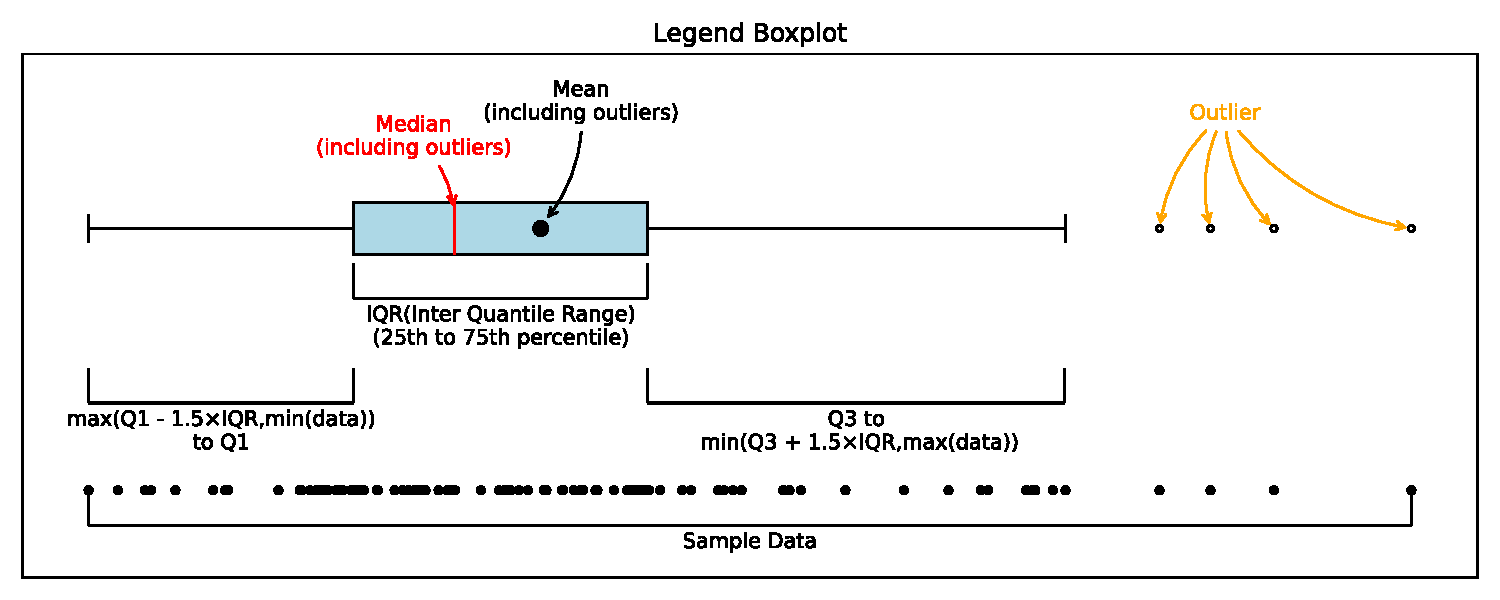
\includegraphics[width=1.\textwidth]{chapters/foundations/images_foundation/legend_boxplot}
    \caption{A boxplot showing the distribution of a toy data set with the important features labeled. Note that the left whiskers is shorted, which indicates that the data is right skewed.}
\end{figure}
Another challenge is the visualisation of the electron density of a molecule. In this work we are
\chapter{Differential Differentials}
In order to optimize the exponents and coefficients of basis sets we are employing differentiable integrals in order to use automatic differentiation and gradient decent to optimize the basis sets. Most commonly used integral implentations like libcint\cite{sun_libcint_2015} are implemented in c++ as the computation of the integrals using the previously introduced recursion relations involves many loops and is computationally expensive as the integrals have to be computed for every combination of shells from every atom with each other. This would make the integrals also very computationally expensive if one would store all recursions in memory at at given time. This is why efficient integral libraries delete or override temporary variables when they are not longer usefull. But this makes it also impossible to use automatic differentiation as they rely on building a complete computational graph through which the gradients can be backpropagated. In order to obtain a differentiable integral computation framework we started with the much less optimized python library for chemical integrals \cite{kim_gbasis_2024}. Their entire framework was build upon the numerical computation package for python numpy\cite{harris2020array}, which could easily be replaced by the popular machine learning framework pytorch\cite{paszke2019pytorch}. As pytorch implements automatic differentiation and gradient decent it is possible to compute the integrals in a differentiable way if all parts of the calculation are done using pytorch. Unfortually these integrals were not very efficient as they involved a large number of operations and lead to an very complicated computational graph.

\subsection{Optimization of the integrals}
The native integral implementation of gbasis involved treating every exponent of a ... as a separate variable and computing the integrals for every combination of them individually. This could be improved by treating all exponents and coefficients of a shell as a single PAo which lets us define them as a single torch Tensor object. As another optimisation procedere all combinations of shells which happend to have the same number of dimentions, so for example in a two center integral all combinations of shells with angular momentum 0 with all possible partners of anglar momentum 1, were concatenated , such that all these integrals could be computed in a single step. This reduces the amount of torch calculations drasticly and lowers the complexity of the resulting computational graph.
Still after these improvements the standart libraries were still orders of magnitudes faster, even when deploying the integrals on gpu.
\chapter{Theoretical Foundations}
This section introduces the fundamentals that are neccesary to understand the following chapters. The section is divided into four parts. First the Density functional theory is introduced, followed by the orbital free DFT formulation. The third part introduces the basis sets that are used in DFT calculations. The last part introduces machine learning and the graphformer model that is used in this thesis.




Methods:
Density functional theory and speciffically kohn sham
Basis sets GTOs and PAOs and their integrals. typical basis sets
Orbital free dft formulation basis sets even tempered, density fitting 
Machine learing
Graphformer  Message passing Graph neural network

\section{Density functional theory}
\subsection{Historical Background}
Kohn-Sham Density Functional Theory (KSDFT) stands as a cornerstone in computational quantum mechanics, revolutionizing our approach to electronic structure calculations. Developed by Walter Kohn and Lu Jeu Sham in 1965 \cite{KohnSham1965}, KSDFT extends the foundational work of Hohenberg and Kohn \cite{HohenbergKohn1964} on Density Functional Theory (DFT).
\subsection{Theoretical Foundation}
The theoretical underpinning of DFT rests on two fundamental theorems proved by Hohenberg and Kohn:
\begin{theorem}
The ground-state properties of a many-electron system are uniquely determined by the electron density $n(\mathbf{r})$.
\end{theorem}
\begin{theorem}
There exists a universal functional of the electron density, $F[n(\mathbf{r})]$, which can be used to find the ground-state energy of the system.
\end{theorem}
These theorems establish that the ground-state energy of a system can be expressed as a functional of the electron density:
\begin{equation}
E[n] = F[n] + \int V_{\text{ext}}(\mathbf{r})n(\mathbf{r})d\mathbf{r}
\end{equation}
where $V_{\text{ext}}(\mathbf{r})$ is the external potential and $F[n]$ is a universal functional independent of the external potential.
\subsection{The Kohn-Sham Approach}
Kohn and Sham proposed a practical approach to apply DFT by introducing a fictitious system of non-interacting particles that generate the same density as the system of interacting particles. This approach involves solving a set of single-particle Schrödinger-like equations, known as the Kohn-Sham equations:
\begin{equation}
\left[-\frac{1}{2}\nabla^2 + V_{\text{eff}}(\mathbf{r})\right]\phi_i(\mathbf{r}) = \epsilon_i\phi_i(\mathbf{r})
\end{equation}
where $\phi_i(\mathbf{r})$ are the Kohn-Sham orbitals and $\epsilon_i$ are their corresponding energies. The effective potential $V_{\text{eff}}(\mathbf{r})$ is defined as:
\begin{equation}
V_{\text{eff}}(\mathbf{r}) = V_{\text{ext}}(\mathbf{r}) + V_{\text{H}}(\mathbf{r}) + V_{\text{xc}}(\mathbf{r})
\end{equation}
Here, $V_{\text{ext}}(\mathbf{r})$ is the external potential, $V_{\text{H}}(\mathbf{r})$ is the Hartree potential, and $V_{\text{xc}}(\mathbf{r})$ is the exchange-correlation potential.
\subsection{Contributions to the Kohn-Sham Energy}
The total energy in the Kohn-Sham formulation can be expressed as:
\begin{equation}
E_{\text{KS}} = T_s[n] + E_{\text{H}}[n] + E_{\text{xc}}[n] + E_{\text{ext}}[n]
\end{equation}
Let us examine each term in detail:
\subsubsection{Kinetic Energy of Non-interacting Electrons}
The kinetic energy of the non-interacting electrons, $T_s[n]$, is given by:
\begin{equation}
T_s[n] = -\frac{1}{2}\sum_i \int \phi_i^*(\mathbf{r})\nabla^2\phi_i(\mathbf{r})d\mathbf{r}
\end{equation}
This term represents the kinetic energy of the Kohn-Sham orbitals.
\subsubsection{Hartree Energy}
The Hartree energy, $E_{\text{H}}[n]$, represents the classical electrostatic interaction energy of the electron density:
\begin{equation}
E_{\text{H}}[n] = \frac{1}{2}\int\int \frac{n(\mathbf{r})n(\mathbf{r'})}{|\mathbf{r}-\mathbf{r'}|}d\mathbf{r}d\mathbf{r'}
\end{equation}
\subsubsection{Exchange-Correlation Energy}
The exchange-correlation energy, $E_{\text{xc}}[n]$, encapsulates all many-body effects beyond the Hartree approximation. Its exact form is unknown, and developing accurate approximations for this term is a central challenge in DFT. Common approximations include:
\begin{itemize}
\item Local Density Approximation (LDA):
\begin{equation}
E_{\text{xc}}^{\text{LDA}}[n] = \int n(\mathbf{r})\epsilon_{\text{xc}}(n(\mathbf{r}))d\mathbf{r}
\end{equation}
where $\epsilon_{\text{xc}}(n)$ is the exchange-correlation energy per particle of a uniform electron gas of density $n$.
\item Generalized Gradient Approximation (GGA):
\begin{equation}
E_{\text{xc}}^{\text{GGA}}[n] = \int f(n(\mathbf{r}), |\nabla n(\mathbf{r})|)d\mathbf{r}
\end{equation}
where $f$ is a function of both the density and its gradient.
\end{itemize}
\subsection{External Potential Energy}
The external potential energy, $E_{\text{ext}}[n]$, represents the interaction of the electrons with the external potential (typically due to the nuclei):
\begin{equation}
E_{\text{ext}}[n] = \int V_{\text{ext}}(\mathbf{r})n(\mathbf{r})d\mathbf{r}
\end{equation}
\section{Self-Consistent Field Method}
The Kohn-Sham equations are solved iteratively using the Self-Consistent Field (SCF) method:
\begin{enumerate}
\item Start with an initial guess for $n(\mathbf{r})$
\item Calculate $V_{\text{eff}}(\mathbf{r})$
\item Solve the Kohn-Sham equations to obtain $\phi_i(\mathbf{r})$
\item Calculate a new density: $n_{\text{new}}(\mathbf{r}) = \sum_i |\phi_i(\mathbf{r})|^2$
\item If $|n_{\text{new}}(\mathbf{r}) - n(\mathbf{r})| < \text{tolerance}$, stop. Otherwise, return to step 2 with $n(\mathbf{r}) = n_{\text{new}}(\mathbf{r})$
\end{enumerate}

\section{Orbital free DFT}
Rooted in the original formulation of Density Functional Theory by Hohenberg and Kohn \cite{HohenbergKohn1964}, Orbital-Free Density Functional Theory (OF-DFT) aims to calculate the ground state properties of a many-electron system directly from the electron density, without the need for individual electronic orbitals.
\subsection{Theoretical Foundation}

Based on equation \eqref{eq:energy_density} the total energy of a system can be expressed as a functional of the electron density $\rho(\mathbf{r})$. The challenge of Orbtial free DFT lies in finding an accurate representation of the kinetic energy functional from equation \eqref{eq:kin} directly from the density, without resorting to orbitals. Historic attemps\cite{thakkar1992comparison,wang1999orbital} at this used numerical approximations. Known approximation include the Thomas-Fermi functional\cite{thomas_fermi_1927} and the von Weizsäcker functional\cite{von_weizsacker_1935}. These functionals were based on the kinetic energy of a non-interacting electron gas and its gradient.
\subsubsection{Thomas-Fermi Functional}
The simplest approximation is the Thomas-Fermi functional:
\begin{equation}
T_{TF}[n] = C_{TF} \int n^{5/3}(\mathbf{r}) d\mathbf{r}
\end{equation}
where $C_{TF} = \frac{3}{10}(3\pi^2)^{2/3}$.
\subsubsection{von Weizsäcker Functional}
The von Weizsäcker functional then adds a additional gradient correction:
\begin{equation}
T_{vW}[n] = \frac{1}{8} \int \frac{|\nabla n(\mathbf{r})|^2}{n(\mathbf{r})} d\mathbf{r}
\end{equation}
\subsubsection{Generalized Gradient Approximation (GGA)}
More sophisticated functionals incorporate higher-order density gradients:
\begin{equation}
T_{GGA}[n] = \int t_{GGA}(n(\mathbf{r}), \nabla n(\mathbf{r}), \nabla^2 n(\mathbf{r}), ...) d\mathbf{r}
\end{equation}

If one can represent the total energy of the system as a function of density, the ground state can be found by minimizing the total energy functional using conventional techniques like gradient descent. With the rise of machine learning in DFT, a promising approach is to learn an empirical approximation of the kinetic energy functional from a large dataset of electronic structure calculations.
While initial attempts by Remme et al. and Imoto et al. \cite{remme_kineticnet_2023,imoto2021order} used grid-based density representations, \textsc{M-OFDFT} \cite{zhang_m-ofdft_2023} pioneered the use of atom-centered basis functions, achieving the first successful prediction of energies with chemical accuracy across a large set of geometries. \textsc{M-OFDFT} also introduced the use of individual Self-Consistent Field (SCF) algorithm steps to generate model labels.
However, these labels were insufficient for the model to emulate the true functional around the ground state accurately enough to allow convergence of the minimization procedure. Instead, the density coefficients tended to drift in unphysical directions, necessitating a complicated halting criterion to generate densities near the ground state.
\subsection{OF-DFT label generation}\label{ofdft_labelgen}
In the following, we will describe the label generation process proposed by the authors of M-OFDFT \cite{zhang_m-ofdft_2023} and the modifications we made to increase training data diversity and improve model convergence.\\
In the following we will use the following conventions:\\
We denote the orbital basis functions as $\{\eta_\mu(\mathbf{r})\}_{\mu=1,...,N_\text{basis}}$, which when contracted with the coefficients $\{C_{i,\mu}\}_{i=1,..,N_\text{electrons},\mu=1,...,N_\text{basis}}$ describe the orbitals $\phi_i(\mathbf{r}) = C_i^\mu \eta_\mu(\mathbf{r})$. The orbitals can be used to calculate the electron density $\rho(\mathbf{r}) = \sum_{i=1}^{N_\text{electrons}}\phi_i(\mathbf{r})^2=\sum_{i=1}^{N_\text{electrons}}C_i^\mu \eta_\mu(\mathbf{r})C_i^\nu \eta_\nu(\mathbf{r}) =  \eta_\mu(\mathbf{r})\Gamma^{\mu,\nu} \eta_\nu(\mathbf{r})$. Where we defined the density matrix $\Gamma^{\mu,\nu} = \sum_{i=1}^{N_\text{electrons}}C_i^\mu C_i^\nu$.\\
To describe the density in the orbital free basis we use another basis set $\{\omega_\mu(\mathbf{r})\}_{\mu=1,...,N_\text{of-basis}}$ with corresponding coefficients $\mathbf{p} =\{p^\mu\}_{\mu=1,...,N_\text{of-basis}}$ which form a linear basis for the density $\rho_\text{OF}(\mathbf{r}) = p^\mu \omega_\mu(\mathbf{r})$.\\
We also use the follwing symbols to denote common basis integrals between the two basis sets following the conventions introduced in section \ref{integral_notation}:
\begin{align}
    W_{\mu\nu} &= \langle\omega_\mu |\omega_\nu\rangle\\
    L_{\mu,\nu\gamma} &= \langle \omega_\mu |\eta_\nu\eta_\gamma\rangle\\
    D_{\alpha,\beta,\gamma,\delta}  &= \langle\eta_\alpha\eta_\beta|\eta_\gamma\eta_\delta\rangle\\
    \tilde{W}_{\mu\nu} &= (\omega_\mu |\omega_\nu)\\
    \tilde{L}_{\mu,\nu\gamma} &= (\omega_\mu |\eta_\nu\eta_\gamma)\\
    \tilde{D}_{\alpha,\beta,\gamma,\delta}  &= (\eta_\alpha\eta_\beta|\eta_\gamma\eta_\delta)\\
    S_{\alpha,\beta} &= \langle \eta_\alpha|\eta_\beta\rangle\\
    {v_{ext}}_\mu &= \int \omega_\mu (r) V_{ext} (r)dr\\
    {V_{ext}}_{\mu,\nu} &= \langle \eta_\mu | V_{ext} (r) | \eta_\nu \rangle
\end{align}
We are now set to describe the label generation process.\\
\subsubsection{Density fitting}\label{into_density_fitting}
Density fitting is a procedure to represent the density produced by the Kohn-Sham orbitals using orbital-free basis functions $\{\omega_\mu(\mathbf{r})\}_\textit{\mu=1,...,N_\text{of-basis}}$, while preserving its electronic properties. This mean calculating $\mathbf{p}(\{C_{i,\mu}\}_{i=1,..,N_\text{electrons},\mu=1,...,N_\text{basis}})$.\\
In chapter \ref{chapter:densityfitting}, we define and evaluate different density fitting algorithms and compare the properties of the densities they produce.\\
\subsubsection{Energy and gradient label generation}
The label for the kinetic energy in coordinates is indirectly calculated by:

\begin{align}
    T_S(\mathbf{p}) = T_S(C) + E_{H}(C) + E_{XC}(C) + E_{ext}(C) - E_{H}(\mathbf{p}) + E_{XC}(\mathbf{p}) + E_{ext}(\mathbf{p}).
\end{align}

We cannot calculate the gradient of the kinetic energy directly from this equation as the orbital free density coefficients $\mathbf{p}$ are dependent on
the coefficients in the orbital basis $\{C_{i,\mu}\}_{i=1,..,N_\text{electrons},\mu=1,...,N_\text{basis}}$ in a nontrivial way.\\
Instead, we make use of the minimization procedure in the KSDFT calculation. Additionally we use a method developed by Manuel Klockow which in each iteration of the self consistent field procedere adds an additional pertubation to the effective potential to increase the diversity of the densities in the labels. In each iteration the next set of orbitals is then computed as follows:

\begin{align}
    \Phi^{k} = \underset{\{\phi_i\}_{i=1}^n \text{orthonormal}}{\text{argmin}} \langle \psi_{\mathbf{\phi}} | \hat T_S | \psi_{\mathbf{\phi}} \rangle + \sum_{k'<k} \pi^{(k')}_k V_{eff}^{k'}[\rho_{[\mathbf{\phi}]}] + V_\text{peturb}^{k}(\rhoPhi)
\end{align}


Where $\pi^{(i)}_k$ are the DIIS coefficients of the KSDFT calculation and

\begin{align}
    V_{eff}^{k'}[\rho_{[\mathbf{\phi}]}] = \int \rho_{[\mathbf{\phi}]}(\mathbf{r}) V_{eff[\rho_{[\mathbf{\phi}^{k'}]}]}(r)dr\\
    V_\text{peturb}^{k}(\rhoPhi) = \int \rhoPhi(\mathbf{r}) v_{\text{peturb},\mu}^{k}\omega_\mu(\mathbf{r})dr
\end{align}
is the effective potential of the $k'$-th iteration integrated over the density of the new density and the pertubation of the effective potential of the $k$th iteration. With $v_{\text{peturb},\mu}^{k} \sim \epsilon_k * \mathcal{N}(1,0)$ and $\omega_\mu$ being basis function in the orbital free basis.
$\epsilon_k$ is then chosen such that starts at the 5 interation and decreases over time.
This is solved using Laplace multipliers:

\begin{align}
    \frac{\delta T_S[\rho_{[\mathbf{\phi}^{k}]}]}{\delta \rho}(\mathbf{r}) + \sum_{k'<k} \pi^{(k')}_k V_{eff}^{k'}(\mathbf{r}) + v_{\text{peturb},\mu}^{k}\omega_\mu(\mathbf{r})= \mu^{(k)}
\end{align}
From here we cannot compute the gradient of the kinetic energy exactly but we can calculate its projection in the plane of constant particle numbers. As in density optimisation our searchspace is restricted to this plane this is sufficient for our purposes.
The projected gradient of the kinetic energy is then calculated as the DIIS weighted average over the projected last few effective potentials:

\begin{align}
    \nabla_\mathbf{p} T_S(\mathbf{p}) &= \int \frac{\delta T_S[\rho_{[\mathbf{\phi}^{k}]}]}{\delta \rho}(\mathbf{r}) \mathbf{\omega}(\mathbf{r}) d\mathbf{r} \\
    &= -\int\sum_{k'<k} \pi^{(k')}_k V_{eff}^{k'}(\mathbf{r}) \mathbf{\omega}v_{peturb,\mu}^{k}\omega_\mu(\mathbf{r})(\mathbf{r}) +\mu^{(k)}\mathbf{\omega}(\mathbf{r})d\mathbf{r} = -{\mathbf{v}}_{eff\{\mathbf{p}^{k'}\}_{k'< k}}+\mu^{(k)}\mathbf{w}\\
    \left( \textbf{I}-\frac{\textbf{w}^{(d)}{\textbf{w}^{(d)}}^T}{{\textbf{w}^{(d)}}^T
        \textbf{w}^{(d)}}\right) \nabla_\mathbf{p} T_S(\mathbf{p}) &= -\left( \textbf{I}-\frac{\textbf{w}^{(d)}{\textbf{w}^{(d)}}^T}{{\textbf{w}^{(d)}}^T
        \textbf{w}^{(d)}}\right){\mathbf{v}}_{eff\{\mathbf{p}^{k'}\}_{k'< k}}\\
    \mathbf{v}_{eff}(\mathbf{p}) &= \nabla_\mathbf{p} (E_{H}(\mathbf{p}) + E_{XC}(\mathbf{p}) + E_{ext}(\mathbf{p}))
\end{align}
These labels for the kinetic energy are then used to train a machine learning model to emulate the kinetic energy functional.\\

\subsection{Preparation of the data}
To prepare the data for machine learning, we employ the same techniques as in the original M-OFDFT \cite{zhang_m-ofdft_2023} paper. We briefly describe their functions here.
\subsubsection{Natrep}
Orthogonalizing the orbital-free basis for more meaningful coefficients.
\subsubsection{Dimensionwise rescaling}
Statistics are calculated for the coefficients of each atom type in the dataset, and the coefficients are rescaled to have a mean of 0 and a standard deviation of 1.
\subsubsection{Local frames}
To make the model rotationally invariant, a local coordinate system is defined for each atom, oriented towards its nearest neighbor. The coefficients are then projected into this local frame.

\section{Basis sets}
In order to represent spacial functions $f:\mathbb{R}^3\right \mathbb{C}$ inside a DFT calculation atom centric basis sets are most commonly used, as they provide anhanced resolution around the nuleii where most of the electron density is concentrated.
\subsection{Contracted atomic orbitals}
Contracted atomic orbitals are defined as a linear combination of a larger primary basis of basis functions centered on atom centers. Formally we can write a contracted atomic orbitals basis function $\eta_{\mu}(\mathbf{r})$ as a weighted sum of the primary basis functions $\tilde\eta_\nu(\mathbf{r})$ where $\mu,\nu$ are belonging to the same Atom.
\begin{align}
    \eta_{\mu} &=\sum\limits_{\nu} A_{\mu,\nu} \tilde \eta_{\nu}
\end{align}
\subsection{Contracted Gaussian Type Orbitals (CGTOs)}
The radial distribution of primary basis functions $\eta_{\mu}(\mathbf{r})$ is typically chosen as Gaussians centered on the same atom at position $\mathbf{R}$ with different exponents, multiplied by spherical harmonics $Y_{lm}$ to introduce angular dependency.
\begin{align}
\eta_{\mu}(\mathbf{r}) &= N(\alpha,m,l) ||\mathbf{r}-\mathbf{R}||^l Y_{lm}(\frac{\mathbf{r}-\mathbf{R}}{||\mathbf{r}-\mathbf{R}||}) e^{-\alpha ||\mathbf{r}-\mathbf{R}||^2}
\end{align}
where $N(\alpha,m,l)$ are normalisation constants.
Gaussian orbitals offer several advantages: they are computationally efficient, easily integrated, and the product of two Gaussians remains a Gaussian, which simplifies many otherwise complex integrals. However, a single Gaussian cannot accurately describe the electron density cusp near the nucleus. To address this, primitive Gaussians are typically contracted to Contracted Gaussian-Type Orbitals (CGTOs) to form a more physically representative basis set. The contraction coefficients $A_{\mu,\nu}$ are fitted to more accurate basis functions like Slater-type orbitals (STOs).
Spherical harmonics provide arbitrary angular resolution and can be formulated in their Cartesian representation as a polynomial of order $l$.
\begin{align}
    ||\mathbf{v}||^l Y_{lm}(\frac{\mathbf{v}}{||\mathbf{v}||}) &= \sum\limits_{a,b,c\in \mathbb{N}_0 a+b+c\leq l} A_{l,a,b,c} v_1^a v_2^b v_3^c
\end{align}
Where $A_{l,a,b,c}$ are constants. This leads to CGTOs just being finite sums of finite polynominals multiplied with gaussians.

\subsection{Integrals}
Most relevant integrals for DFT involve integrals over products of gaussians which can be computed analytically. Examples are the overlap integral $\langle \eta_{\mu}|\eta_{\nu}\rangle$, the kinetic energy integral $\langle \nabla \eta_{\mu}|\nabla \eta_{\nu}\rangle$, the electron-nucleus integral $\langle \eta_{\mu}|\frac{Z}{||\mathbf{r}-\mathbf{R}||}|\eta_{\nu}\rangle$ as well as the hartree integral $(\eta_{\mu}\eta_{\nu}|\eta_\gamma\eta_\delta)$. While these closed form solutions exist they still involve many repeated recursion relations and can be very compute intensive for larger molecules. Other more complicated integrals, such as the Thomas Fermi functional or the von Weizsäcker functional, as well as practically all exchange correlation functionals, are usually computed numerically on a sufficently large grid. In this work we are using the implementationa of the libcint library \cite{sun_libcint_2015} to compute these integrals, when they don't have to be differentiable.


\section{Machine Learning}
Machine Learning is since .. Nobel price 2024


\section{Graph Neural Networks}
Graph neural networks are a special Variant of Neural networks that apply to graph shaped data.
In our case the graph is the molecular structure of the system that we want to model. Each atom functions as a node in the graph which contains information about the local density around this atom in form of the coefficients of the basis function that centered on the atom. The Edges of the graph contain information in form of the distance towards the next atom. These distances can be embedded in the edge features of the graph neural network.

\subsection{Messagepassing Neural Network}
Message Passing Neural Networks (MPNNs) operate on graph-structured data G = (V, E), where V is the set of nodes and E is the set of edges. The core of MPNNs is the message passing operation, defined as:

\begin{align}
m_t^{(v)} &= \text{AGG}\left(\{M_t(h_t^{(v)}, h_t^{(u)}, e_{vu}) \mid u \in N(v)\}\right) \\
h_{t+1}^{(v)} &= U_t(h_t^{(v)}, m_t^{(v)})
\end{align} 
    

where $h_t^(v)$ is the hidden state of node $v$ at time step $t$, $e_vu$ is the edge feature between nodes $v$ and $u, N(v)$ is the neighborhood of $v, M_t$ is the message function, AGG is an aggregation function (e.g., sum, mean, max), and $U_t$ is the update function. These operations are performed for $T$ time steps to capture higher-order interactions in the graph.

\subsubsection{Embeddings}
The atomic number of every atom is one hot encoded into a vector which length the number of distinct atomtypes in the dataset is. The distance between the atoms Is embedded using besselfunction following the approach of \cite{https://arxiv.org/pdf/2003.03123}. See figure \ref{fig:bessel_embedding}
\begin{align}
    \tilde{e}_{\text{RBF},n}(d) &= \sqrt{\frac{2}{c}}\frac{\sin(\frac{\omega_n }{c})}{d}\hspace{2cm} \omega_n :=(n+1)d\pi\\
    u(d)&= 1-\frac{(p+1)(p+2)}{2}d^p + p(p+2)d^{p+1}-\frac{p(p+1)}{2}d^{p+2}
\end{align}
Where we choose p = 1 and c = 6, as most of the bonds in our dataset are shorter than 6 Angstrom as can be seen in figure \ref{fig:bond_length}. The distance embedding is then multiplied with the one hot encoded atomic number of the atom to get the final edge feature.

\begin{figure}
    \centering
    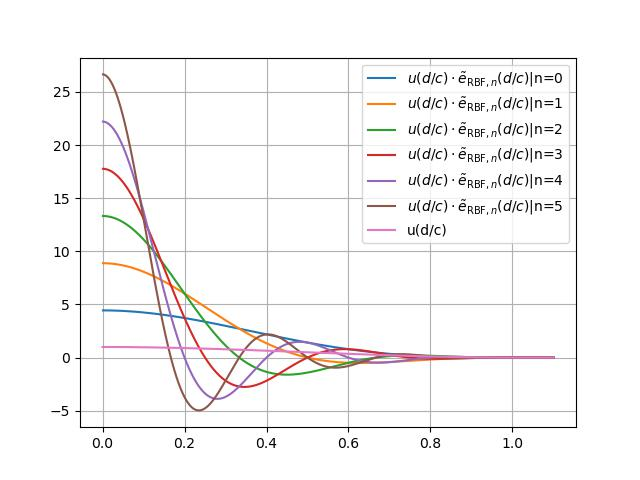
\includegraphics[width=0.8\textwidth]{chapters/foundations/images_foundation/bessel_embedding}
    \caption{The initial basis function used for the distance embedding in the graph neural network.}
    \label{fig:bessel_embedding}
\end{figure}
\begin{figure}
    \centering
    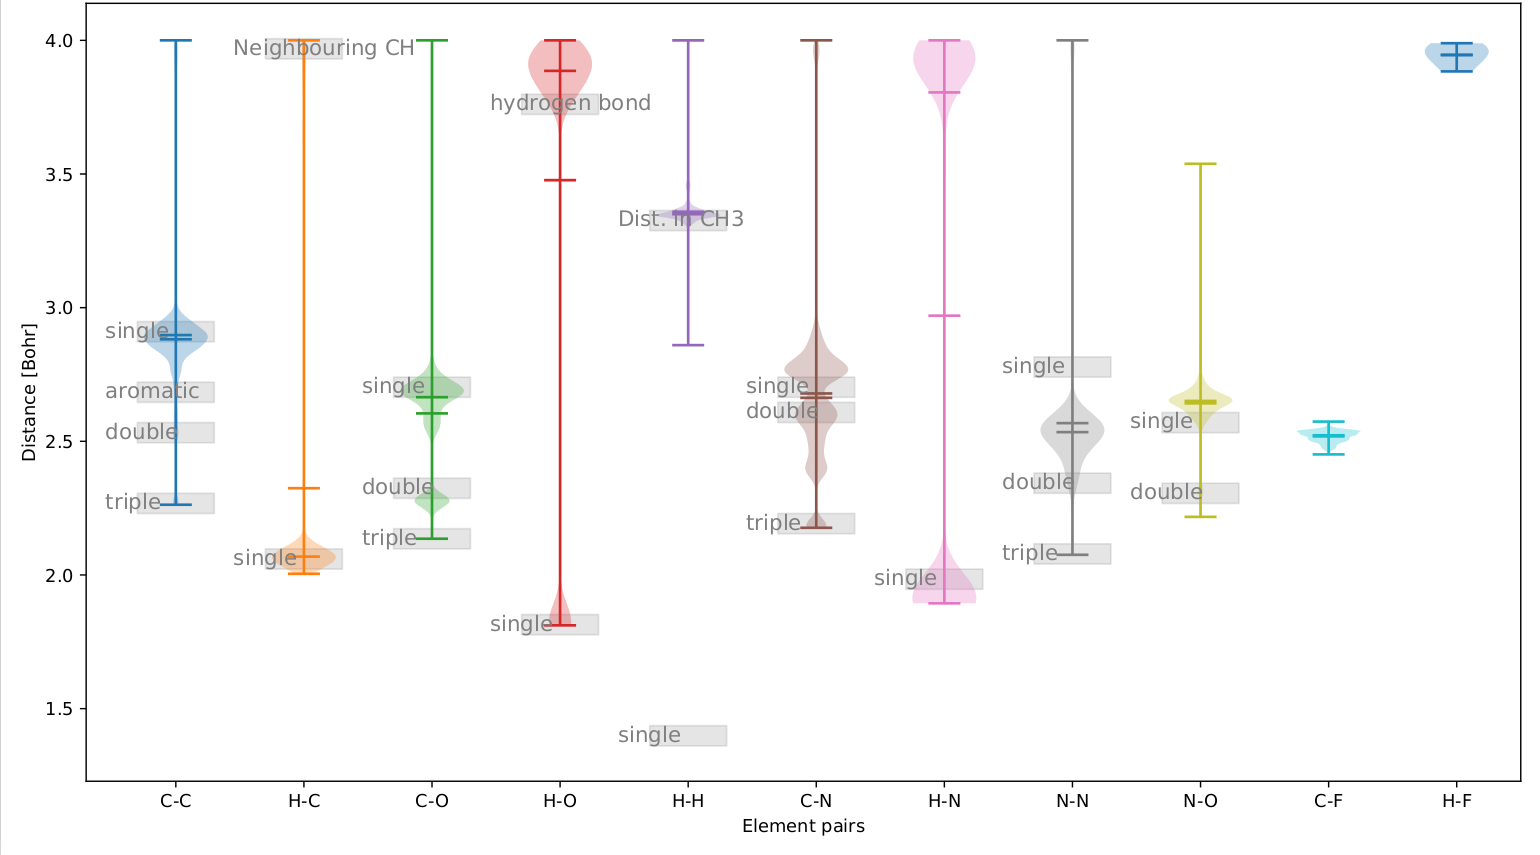
\includegraphics[width=0.8\textwidth]{chapters/foundations/images_foundation/bondlength}
    \caption{The average Bondlength appearing in QM9(Credit Tobias)}
    \label{fig:bond_length}
\end{figure}
For the final embedding of the edge features the one hot encoded atomic number of the incomming and outcomming atom is concatenated with the distance embedding. This is then passed through a short MLP\cite{mlp} with scip connection:
%\begin{align}
%        h_i:= \text{HOTONE(z_i)}\in R^{n_z}\\
%        e_{\text{edge embedding},i,j}^{(0)} = \sigma((h_i||h_j||\text{emb_{ij}})W_{\text{edge}}+b_{\text{edge}})\\
%    e_{\text{edge embedding},i,j}^{(1)} &= u(d_{i,j})(x_{\text{edge embedding}}^{(0)} + \text{MLP}(x_{\text{edge embedding}}^{(0)}))
%\end{align}
These edge features are then aggregated into node features using an aggregation function. The Node features are then futher processed.
\begin{align}
    n_{node_{features},i}^{(0)} &= \text{AGG}(e_{\text{edge embedding},i,j}^{(1)})_i + h_{i}W_{\text{node}} + b_{\text{node}} \\
    n_{node_{features},i}^{(l+1)} &= \text{BatchNorm}(n_{node_{features},i}^{(l)} + \text{MLP}(n_{node_{features},i}^{(l)}))
\end{align}
Then iterativly new edge messages are contructed from these node features and again aggregated to node features:
\begin{align}
    e_{\text{edge embedding},i,j}^{(l+1)} &= \text{MLP}(n_{node_{features}i}^{(l)}||n_{node_{features},j}^{(l)}||e_{\text{edge embedding}i,j}^{(l)})\\
    n_{node_{features},i}^{(l+1)} &= \text{AGG}(e_{\text{edge embedding},i,j}^{(l+1)})_i + n_{node_{features},i}^{(l)}
\end{align}
\subsection{Graphformer}
The architecture for the much more expressive model used for OFDFT is the Graphformer. The Graphformer is a transformer like architecture that operates on graph structured data, in this case a complete graph but takes into account the distances between different nodes in its attention module. \cite{Graphformer}.
We also intotroduce a Atomic reference module as it was done in Mofdft\cite{zhang_m-ofdft_2023}.

\chapter{Density Fitting}
As intoduced in Chapter \ref{density_fitting_theory}
density fitting is ma method that attemps to reproduce the physical properties of a electron density produced by a set of orbitals by using a orbital free basis set.
In the following the different denisty fitting methods are introduced and compared.
\subsection{Metrics}
To evaluate the different density fitting methods the following metrics are used:
\begin{enumerate}
    \item Mean Absolute Error (MAE) of the Energies (Hartree, External, xc, kinetic)
    \item Mean Absolute Error (MAE) of the of the number of electrons $N = \int \rho(\mathbf{r}) d\mathbf{r}$
    \item The L2 Norm of the difference in densities $\text{L2}[\rho-\rho'] = \sqrt{\int (\rho(\mathbf{r})-\rho'(\mathbf{r}))^2} d\mathbf{r}$
    \item The L1 Norm of the difference in densities $\text{L1}[\rho-\rho'] = \int |\rho(\mathbf{r})-\rho'(\mathbf{r})| d\mathbf{r}$
    \item The Gradient of the total energy at the ground state (Interesting for convergence)
    \item The L1 Norm of negative values in the fitted density $\text{L1}[\rho'] = \int \text{RELU}(-\rho'(\mathbf{r})) d\mathbf{r}$
    \item The Hartree energy of the residual density $\text{Hartree}[\rho-\rho'] = \int \int \frac{(\rho(\mathbf{r})-\rho'(\mathbf{r}))(\rho(\mathbf{r'})-\rho'(\mathbf{r'}))}{|\mathbf{r}-\mathbf{r'}|}d\mathbf{r}d\mathbf{r'}$
    \item Stability of the fitted density coefficients (std of the coefficients)
\end{enumerate}
\subsection{Density fitting methods}
Here the different density fitting methods which were considert are introduced and compared.
The derivation are include in Appendix \ref{appendix:density_fitting}
\subsubsection{Overlap Density fitting}
\begin{align}
        \mathcal{L}(\mathbf{p}) &= \mathbf{p} W \mathbf{p} - 2 \mathbf{p}\bar { L} \bar\Gamma + \bar\Gamma \mathbf{D}\bar\Gamma
\end{align}

\subsubsection{Hartree Density fitting}
Minimizes the following metric:
\begin{align}
        \mathcal{L}(\mathbf{p}) &= \mathbf{p} \tilde{W} \mathbf{p} - 2 \mathbf{p}\bar {\tilde L} \bar\Gamma + \bar\Gamma \tilde{\mathbf{D}}\bar\Gamma
\end{align}
Which results in the following formula for the fitted density coefficients:
\begin{align}
    \mathbf{p}&=\tilde{W}^{-1}\bar {\tilde L} \bar\Gamma\\
\end{align}


\subsubsection{Hartree+External Density Fitting}
\begin{align}
        \mathcal{L}(\mathbf{p}) &= \mathbf{p} \tilde{W} \mathbf{p} - 2 \mathbf{p}\bar {\tilde L} \bar\Gamma + \bar\Gamma \tilde{\mathbf{D}}\bar\Gamma + (\mathbf{p}\mathbf{v}_{ext}-\bar\Gamma \bar{V}_{ext})^2
\end{align}
\begin{align}
    A&:=\tilde{W}+\mathbf{v}_{ext}\mathbf{v}_{ext}^T\\
    \mathbf{p}&:=A^{-1}\left(\bar {\tilde L}+\mathbf{v}_{ext}\bar{V}_{ext}\right) \bar\Gamma\\
\end{align}

\subsubsection{Hartree+External Density Fitting MOFDFT-Version}
\begin{align}
\mathcal{L}(\mathbf{p}) &= \mathbf{p} \tilde{W} \mathbf{p} - 2 \mathbf{p}\bar {\tilde L} \bar\Gamma + \bar\Gamma \tilde{\mathbf{D}}\bar\Gamma + (\mathbf{p}\mathbf{v}_{ext}-\bar\Gamma \bar{V}_{ext})^2\\
&\left(\begin{array}{c}\tilde{W}\\v_{ext}^T\end{array}\right) \mathbf{p} =  \left(\begin{array}{c}\tilde{L} \bar{\Gamma} \\ \bar{\Gamma}\bar{V}_{ext}\end{array}\right)
\end{align}


\subsubsection{Hartree+External Density Fitting with enforced electron number}
\begin{align}
    \mathcal{L}(\mathbf{p},\mu) &= \mathbf{p} \tilde{W} \mathbf{p} - 2 \mathbf{p}\bar {\tilde L} \bar\Gamma + (\mathbf{p}\mathbf{v}_{ext}-\bar\Gamma \bar{V}_{ext})^2+\mu(\mathbf{p}\mathbf{w}-\bar\Gamma\bar S)\\
    A^{-1}\left(\bar {\tilde L} + \mathbf{v}_{ext} \bar{V}_{ext}- \mathbf{w}\frac{\mathbf{w}A^{-1}\bar {\tilde L} +\mathbf{w}A^{-1}\mathbf{v}_{ext} \bar{V}_{ext}-\bar S}{\mathbf{w}A^{-1}\mathbf{w}}\right)\bar\Gamma\\
\end{align}



\subsubsection{Hartree Density Fitting with enforced electron number and enforced external energy}
\begin{align}
    \mathcal{L}(\mathbf{p},\mu,\nu) &= \mathbf{p} \tilde{W} \mathbf{p} - 2 \mathbf{p}\bar {\tilde L} \bar\Gamma + \nu(\mathbf{p}\mathbf{v}_{ext}-\bar\Gamma \bar{V}_{ext})+\mu(\mathbf{p}\mathbf{w}-\bar\Gamma\bar S)\\
\end{align}


\subsubsection{Hartree+External Density Fitting MOFDFT-Version with soft enforced electron number}
\begin{align}
    \mathcal{L}(\mathbf{p}) &= \mathbf{p} \tilde{W} \mathbf{p} - 2 \mathbf{p}\bar {\tilde L} \bar\Gamma + \bar\Gamma \tilde{\mathbf{D}}\bar\Gamma + (\mathbf{p}\mathbf{v}_{ext}-\bar\Gamma \bar{V}_{ext})^2 + (\mathbf{p}\mathbf{w}-\bar\Gamma \bar{S})^2
\end{align}
\begin{align}
    \left(\begin{array}{c}\tilde{W}\\\mathbf{v}_{ext}^T\\\mathbf{w}^T\end{array}\right) \mathbf{p} =  \left(\begin{array}{c}\tilde{L} \bar{\Gamma} \\ \bar{\Gamma}\bar{V}_{ext}\\\bar S\bar \Gamma\end{array}\right)
\end{align}


\subsubsection{Hartree+External Density Fitting MOFDFT-Version with hard enforced electron number}
\begin{align}
    \mathcal{L}(\mathbf{p}) &= \left\lVert\left(\begin{array}{c}\tilde{W}\\v_{ext}^T\end{array}\right) \mathbf{p} - \left(\begin{array}{c}\tilde{L} \bar{\Gamma} \\ \bar{\Gamma}\bar{V}_{ext}\end{array}\right)\right\rVert^2 + \lambda (\mathbf{w}\mathbf{p}-N)
\end{align}



\subsubsection{Overlap Density fitting with enforced electron number}
\begin{align}
    \mathcal{L}(\mathbf{p},\mu) &= \mathbf{p} \tilde{W} \mathbf{p} - 2 \mathbf{p}\bar {\tilde L} \bar\Gamma + (\mathbf{p}\mathbf{v}_{ext}-\bar\Gamma \bar{V}_{ext})^2+\mu(\mathbf{p}\mathbf{w}-\bar\Gamma\bar S)\\
    A^{-1}\left(\bar {\tilde L} + \mathbf{v}_{ext} \bar{V}_{ext}- \mathbf{w}\frac{\mathbf{w}A^{-1}\bar {\tilde L} +\mathbf{w}A^{-1}\mathbf{v}_{ext} \bar{V}_{ext}-\bar S}{\mathbf{w}A^{-1}\mathbf{w}}\right)\bar\Gamma\\
\end{align}



\subsubsection{Overlap Density fitting with enforced electron number and enforced external energy}
\begin{align}
    \mathcal{L}(\mathbf{p},\mu,\nu) &= \mathbf{p} \tilde{W} \mathbf{p} - 2 \mathbf{p}\bar {\tilde L} \bar\Gamma + \nu(\mathbf{p}\mathbf{v}_{ext}-\bar\Gamma \bar{V}_{ext})+\mu(\mathbf{p}\mathbf{w}-\bar\Gamma\bar S)\\
\end{align}

The following plot shows the difference of the metrics evaluated on the first 1000 Molecules of QM9.

Insert plot here

A more detailed Table of the found falues for the different values can be found in the appendix\cite appendix.

\begin{figure}[h]
    \centering
    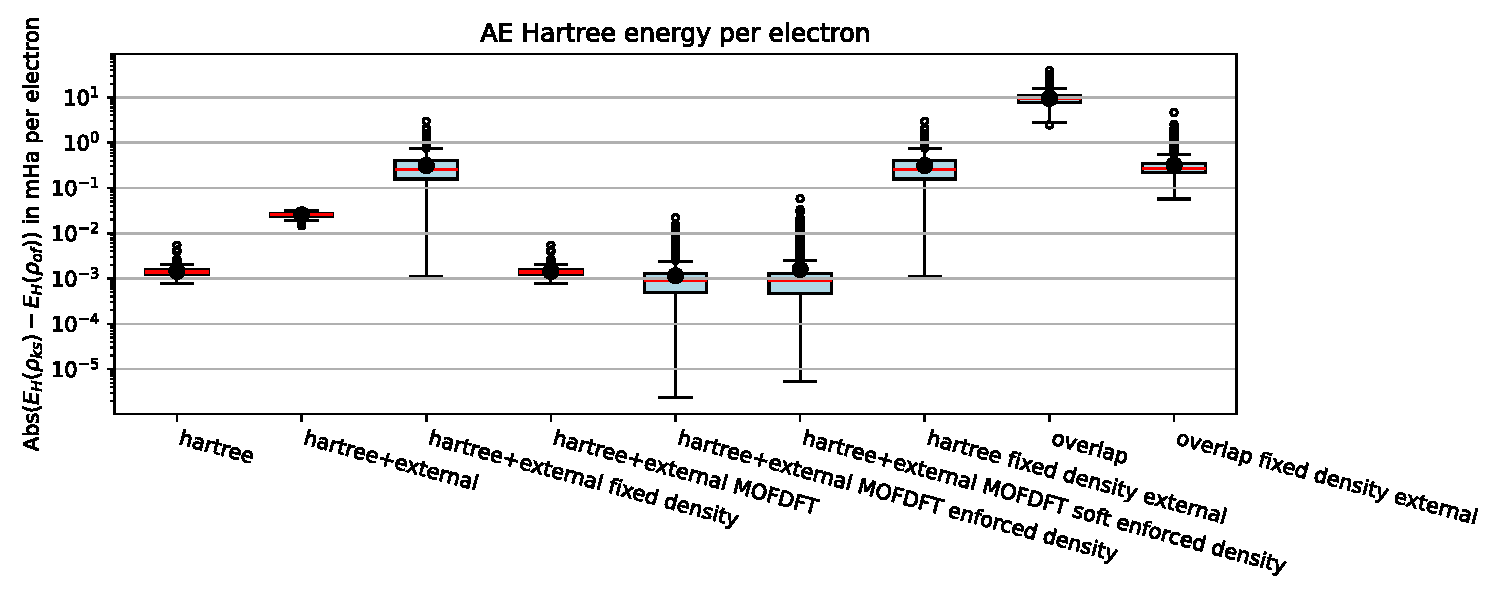
\includegraphics[width=0.5\textwidth]{chapters/results/results_images/AE_hartree_energy_on_even_tempered_2.5}
    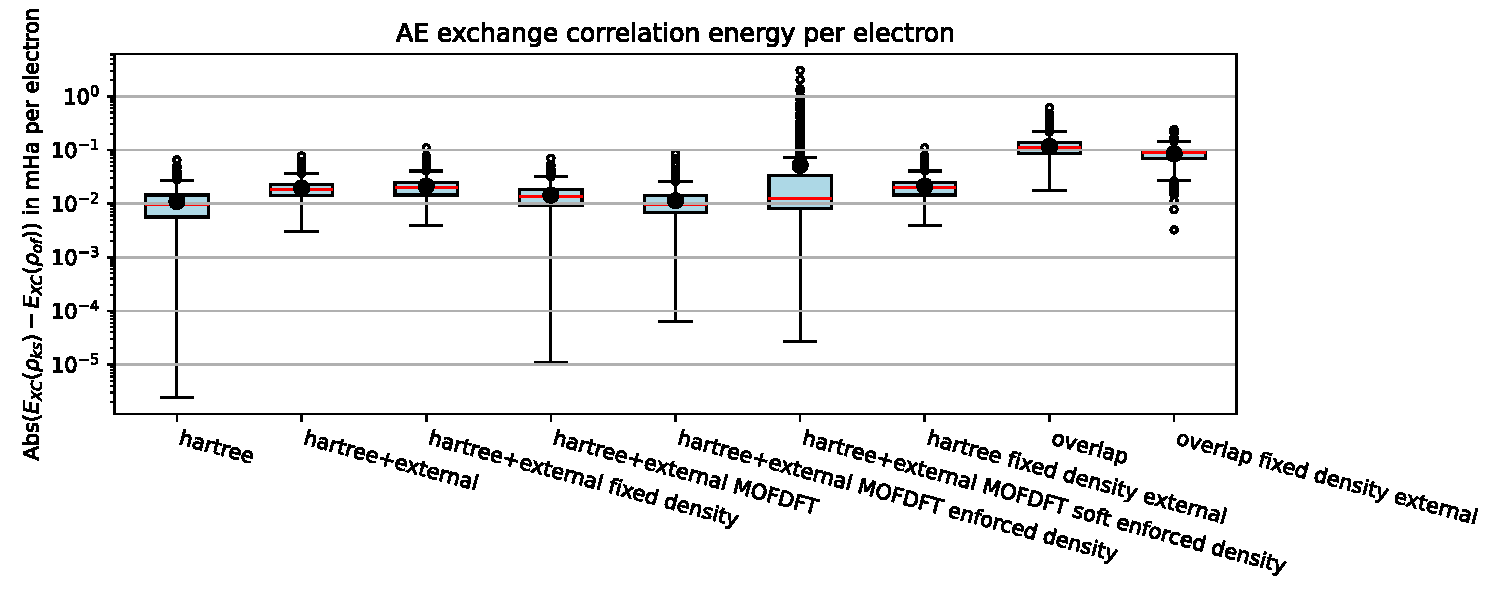
\includegraphics[width=.49\textwidth]{chapters/results/results_images/AE_xc_energy_on_even_tempered_2.5}
    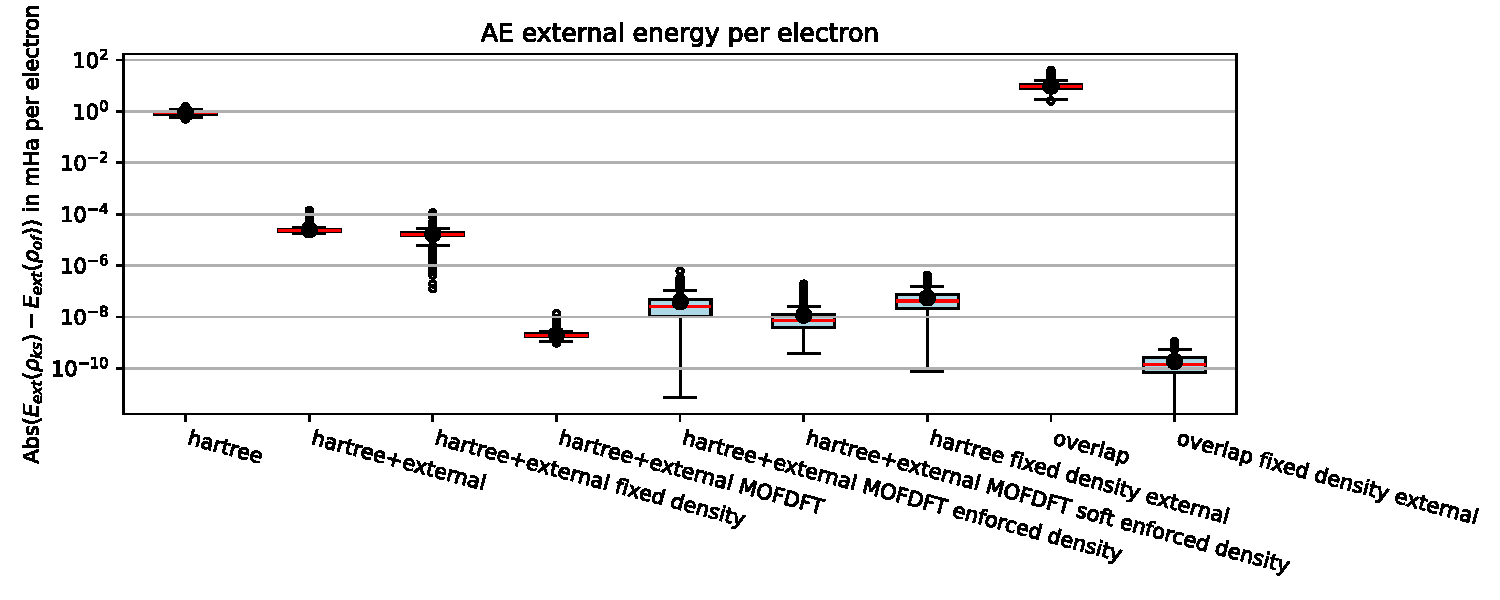
\includegraphics[width=.5\textwidth]{chapters/results/results_images/AE_ext_energy_on_even_tempered_2.5}
    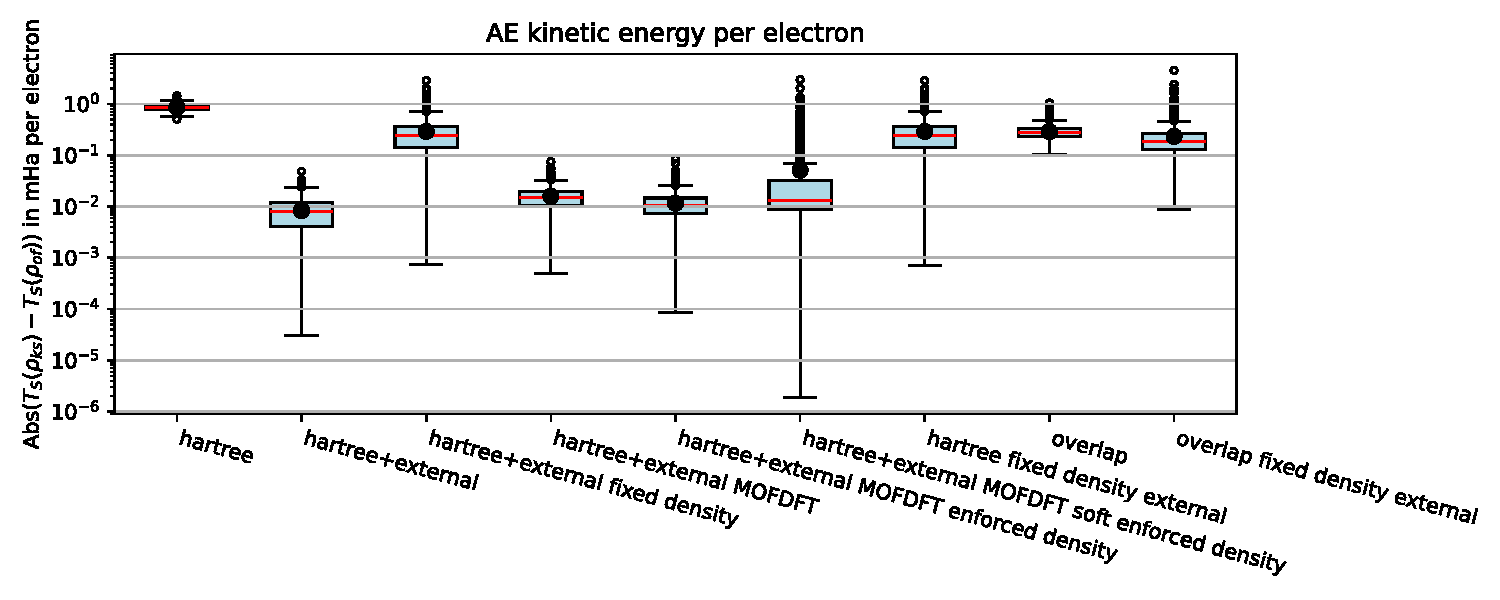
\includegraphics[width=.49\textwidth]{chapters/results/results_images/AE_kin_energy_on_even_tempered_2.5}
    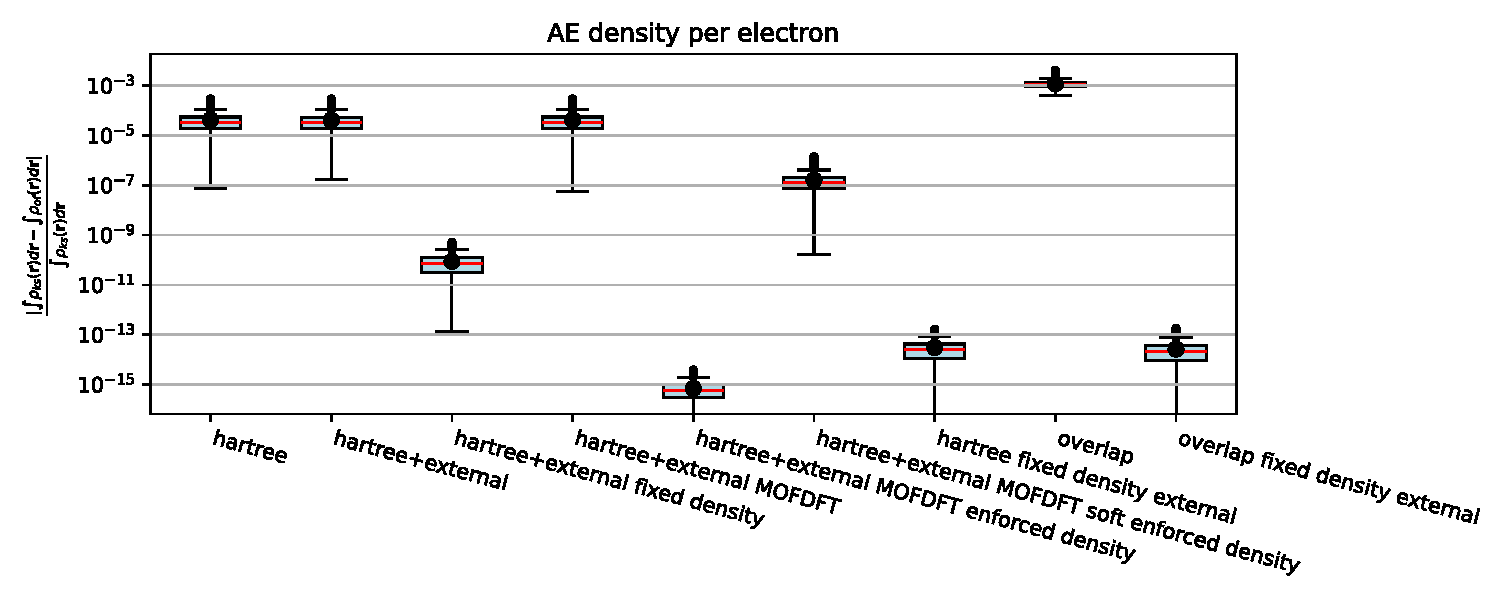
\includegraphics[width=.5\textwidth]{chapters/results/results_images/AE_density_on_even_tempered_2.5}
    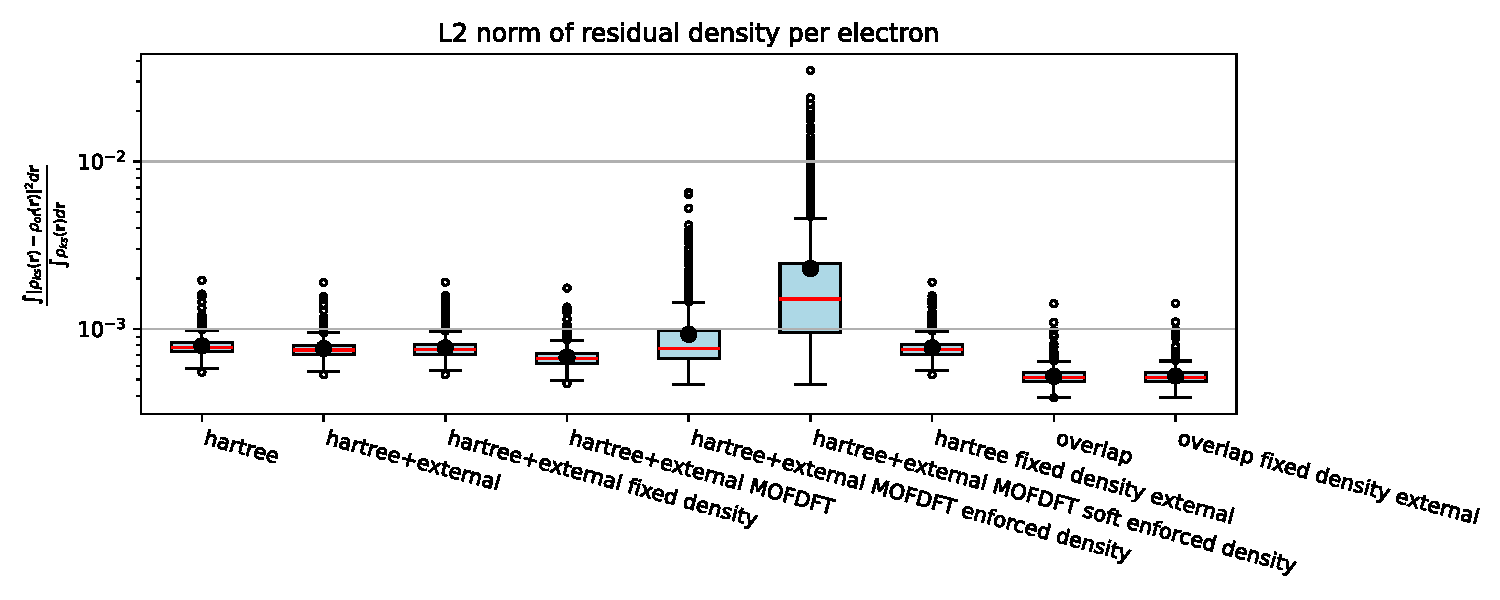
\includegraphics[width=0.49\textwidth]{chapters/results/results_images/L2_residual_densities_on_even_tempered_2.5}
    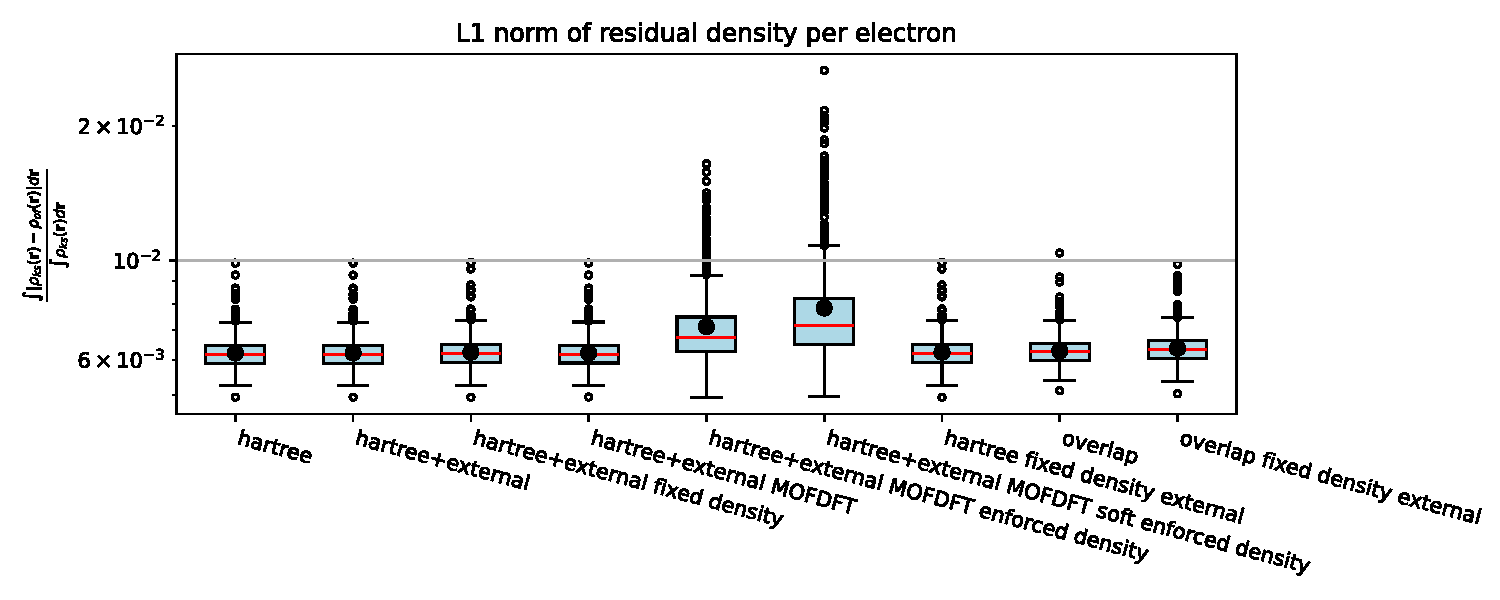
\includegraphics[width=0.5\textwidth]{chapters/results/results_images/L1_residual_densities_on_even_tempered_2.5}
    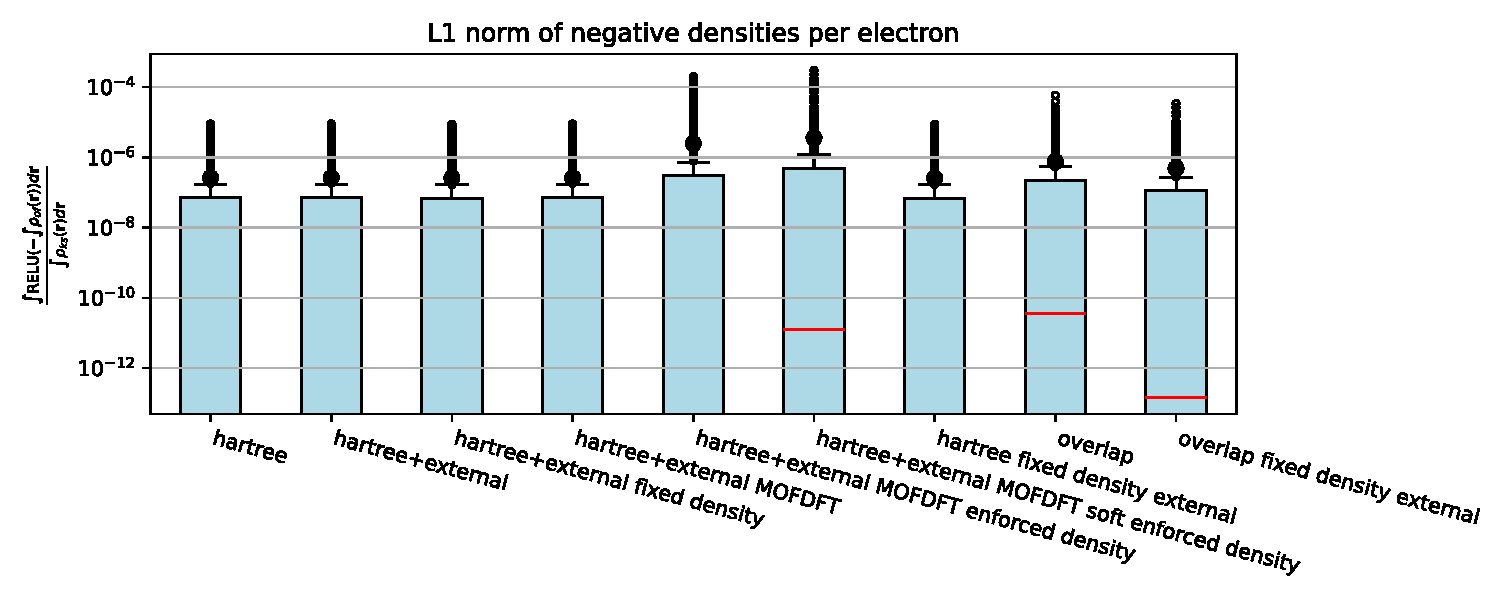
\includegraphics[width=0.49\textwidth]{chapters/results/results_images/L1_negative_densities_on_even_tempered_2.5}
    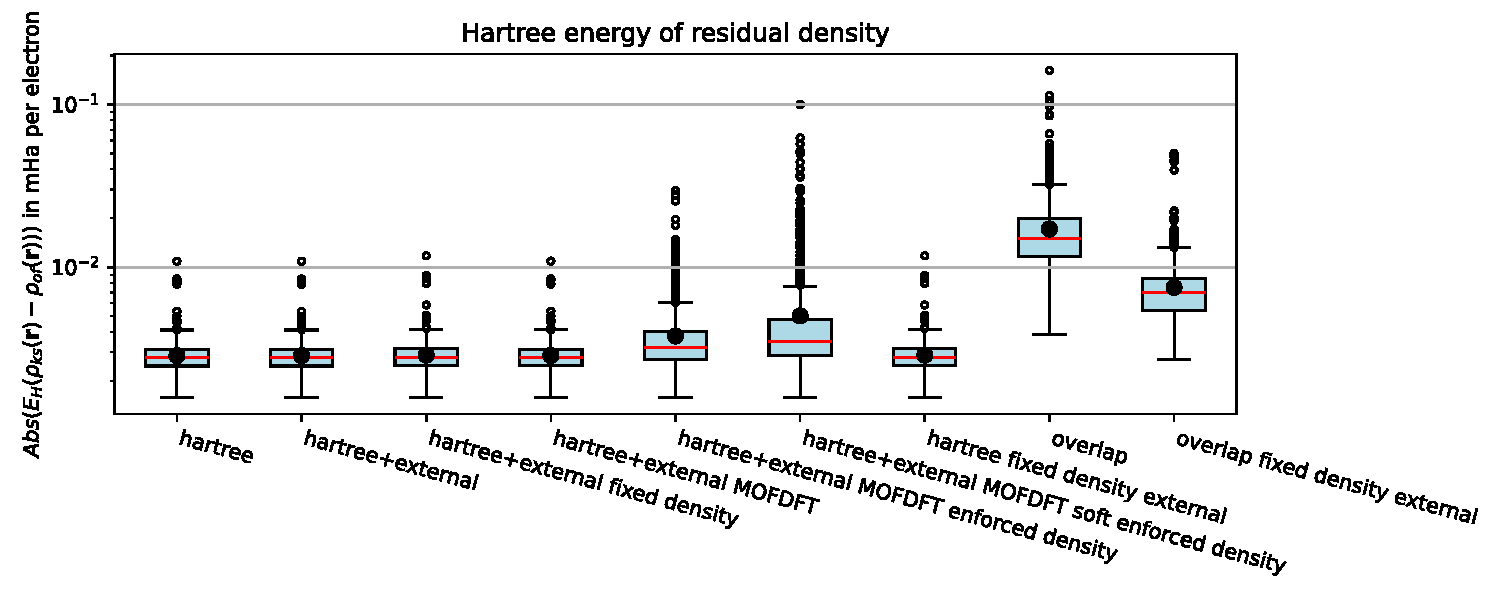
\includegraphics[width=0.5\textwidth]{chapters/results/results_images/L2_residual_hartree_on_even_tempered_2.5}
    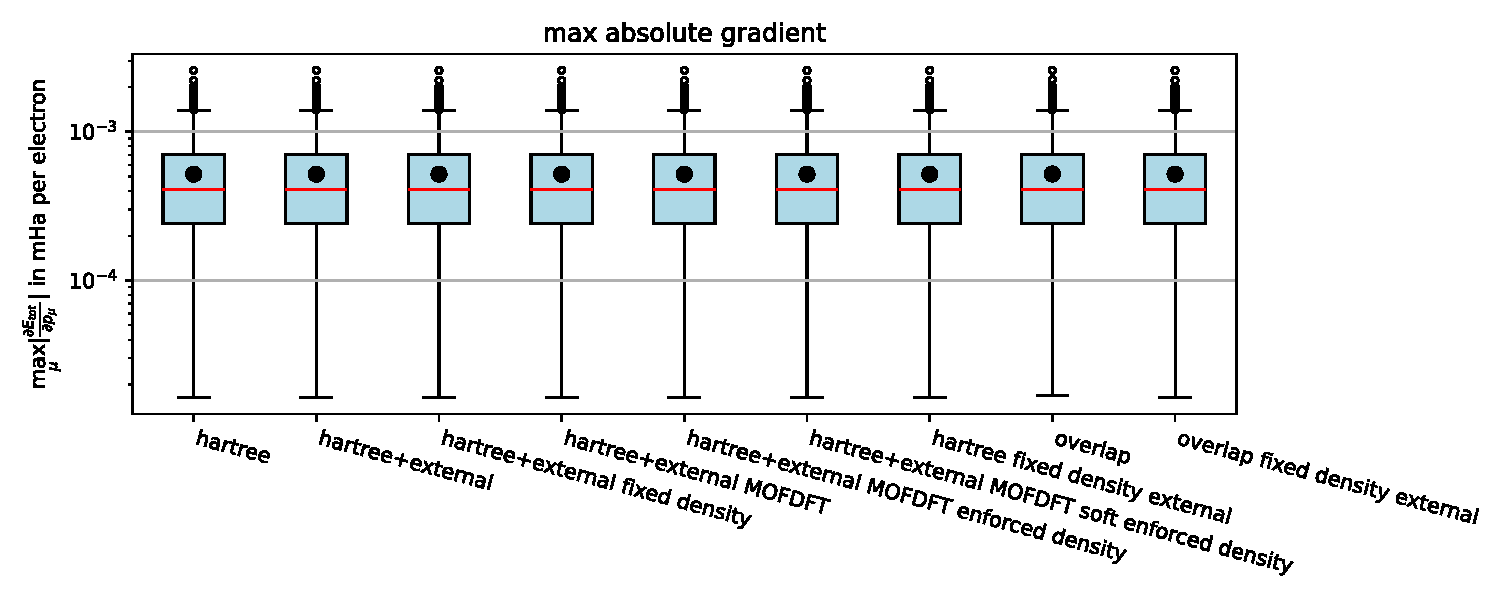
\includegraphics[width=0.49\textwidth]{chapters/results/results_images/max_abs_gradient_on_even_tempered_2.5}
    \includesvg[width=0.5\textwidth]{chapters/results/results_images/var_density_fitting}
    \caption{A plot of the different metrics evaluated on the first 1000 Molecules of the QM9 dataset}
    \label{fig:my_label}
\end{figure}

\begin{figure}[h]
    \centering
    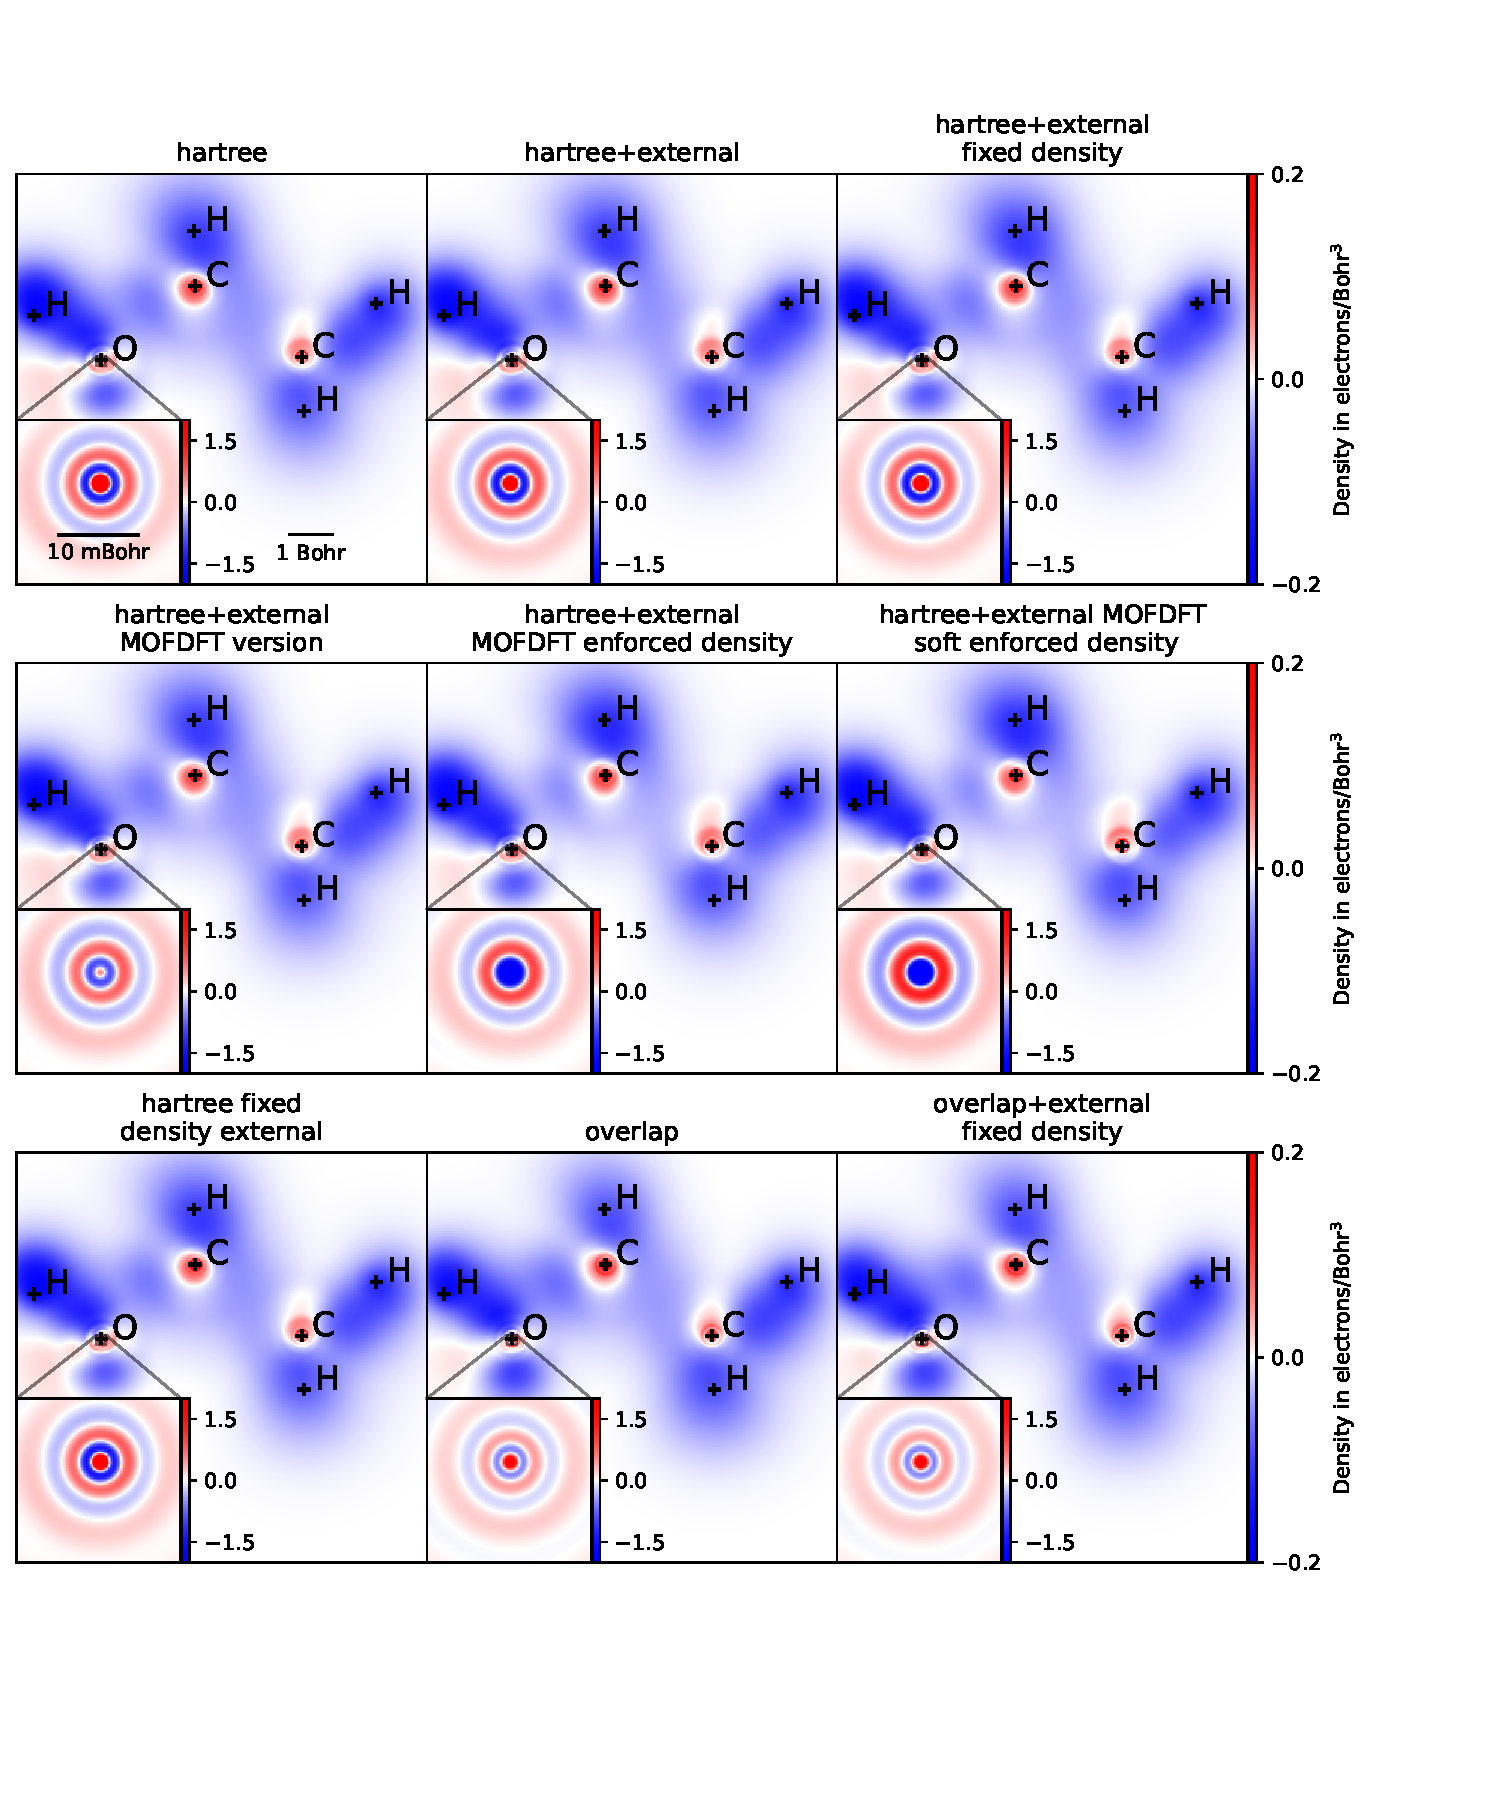
\includegraphics[width=1\textwidth]{chapters/results/results_images/density_fitting_slices}
    \caption{A plot of the different metrics evaluated on the first 1000 Molecules of the QM9 dataset}
    \label{fig:my_label2}
\end{figure}








\chapter{Orbital free basis set fitting}
Apart from the applied density fitting method, the chosen orbital-free basis set arguably has an even greater impact on the accuracy of the density-fitted density. The commonly used even-tempered basis sets are reliable but often inefficient for defining an orbital-free basis. Their simple construction algorithm \cite{const} broadly covers the possible density space without refinement.

To improve the performance of our orbital-free basis set, it is sensible to adopt a basis set with higher resolution in regions where density fluctuates more rapidly. We construct this improved basis by beginning with an even-tempered set and using differentiable integrals and autograd.

\section{Using differentiable integrals to optimize an orbital free basis set}
Given differentiable basis integrals, we can describe the complete density fitting procedere in a completely differentiable way. For a given target density we want to optimize the L2 norm of the fitted density, so we are going to start with the overlap formulation of density ftting defined in \eqref{overlap_eq}. Other formulations using the residual hartree energy can also be easily formulated but they these integrals are much more costly to compute. We also found this formulation to be sufficient to optimize the relevant metrics to an acceptable level.
\begin{align}
    \mathcal{L}[\rho] &= \min_{\rho'}\left(||\rho-\rho'||_{\text{L2}}\right)\\
    & = \min_{\{p_{\mu}\}_{\mu \in 1,...,n_b}} \mathbf{p}W \mathbf{p} - 2 \mathbf{p} \bar L \bar\Gamma + \bar\Gamma \bar D \bar\Gamma\\
    & = \left[\mathbf{p} W \mathbf{p} - 2 \mathbf{p} \bar L \bar\Gamma+ \bar\Gamma \bar D \bar\Gamma\right]_{\mathbf{p} = W^{-1}\bar{L}\bar\Gamma}\\
    & = \bar \Gamma \bar L ^T W^{-1} \bar L \bar \Gamma - 2 \bar \Gamma \bar L^T W^{-1} \bar L \bar \Gamma + \bar \Gamma \bar D \bar \Gamma\\
    & = - \bar \Gamma \bar L^T W^{-1} \bar L \bar \Gamma + \bar \Gamma \bar D \bar \Gamma
\end{align}
We can now insert the dependency of our integrals on the exponents $\{\mathbf{\alpha}_Z\}_{Z\in \text{H,C,N,O,F}}$ for the gaussian basis functions for each atom.
The dependent integrals are the two center integral $W_{\mu,\nu}(\mathbf{\alpha}) = \langle \omega_\mu(\mathbf{\alpha})|\omega_\nu(\mathbf{\alpha})\rangle$
 and the three center overlap integral $L_{\mu,\gamma\sigma}(\mathbf{\alpha}) = \langle \omega_\mu(\mathbf{\alpha})|\eta_\gamma\eta_\sigma\rangle$. The 4 center overlap integral $D$ does not depend on the orbital free basis functions $\omega_\mu(\mathbf{\alpha})$ and can therefor be omitted from the final loss. For a single molecule geometry $\mathcal{M}$ we can define now our loss as
 \begin{align}\label{loss_basis_set_fitting}
    \text{Loss}_\text{molecule}(\mathcal{M}, \Gamma,\mathbf{\alpha}) & = - \bar \Gamma \bar L_{\mathcal{M}}^T(\mathbf{\alpha}) W_{\mathcal{M}}^{-1}(\mathbf{\alpha}) \bar L_{\mathcal{M}}(\mathbf{\alpha}) \bar \Gamma
 \end{align}
The loss of our entire dataset $\{\mathcal{M}_i,\Gamma_i\}_{i\in 1,...,N_{\text{molecules}}}$, containing the atomic structures and ground state densities, amounts to:
\begin{align} \label{loss_dataset_basis_set_fitting}
    \text{Loss}(\{\mathcal{M}_i,\Gamma_i\}_{i\in 1,...,N_{\text{molecules}}},\mathbf{\alpha}) = \sum\limits_{i=1}^{N_{\text{molecules}}} \text{Loss}_\text{molecule}(\mathcal{M}_i, \Gamma_i,\mathbf{\alpha})
\end{align}
For the atomic structures, we used molecules from the popular dataset QM9\ref{QM9}. For the target density, we again used the ground state density of molecules generated by a Kohn-Sham calculation using the PBE exchange-correlation functional and the "6-31G(2df,p)" basis set for the orbitals.
As our entire framework is written in PyTorch and is differentiable, the gradients of the loss in the direction of the individual exponents can be computed using PyTorch's autograd. We then optimize the exponents by minimize our loss function \eqref{loss_dataset_basis_set_fitting} using stochastic gradient descent.
To summarize our training setup:
We perform the entire training loop of building the integrals, computing the loss, and backpropagation on a single GPU. As the integrals require significant RAM (~20GB), we are restricted to a batch size of 1. We trained for approximately 20,000 steps. As the number of steps and parameters (~100) is much smaller than the number of training samples in the dataset (~100,000), we view the risk for overfitting to be very low.
\subsection{Comparison of performance of fitted basis sets with vanilla even-tempered basis sets}
We compare several fitted basis sets originating from even-tempered basis sets with $\beta$ equal to 3 or 2.5 using the same metrics that we used for the different density fitting methods (Section \ref{metrics}). We are going to compare them using the density fitting method hartree+external MOFDFT, which we introduced in the previous chapter \ref{chapter:densityfitting}.
\section{Additional Side Losses}
Using the previously mentioned loss \ref{loss_basis_set_fitting} alone isn't sufficient to guarantee that the fitted basis set produces stable labels. This is evident in the strongly increased standard deviation of some coefficients. In practice, this leads to slower and worse training. The cause of this instability becomes apparent when examining the individual metrics.
To counteract this behavior, we introduce additional side losses on the fitted coefficients $\mathbf{p}(\mathbf{\alpha}) = W^{-1}(\mathbf{\alpha}) \bar L(\mathbf{\alpha}) \bar \Gamma$ during training. These side losses are meant to regularize the exponents by ensuring more stable coefficients. We introduce the following side losses:
 \begin{align}
    \text{Loss}_\text{Coeffs}(\mathcal{M},\mathbf{p}(\mathbf{\alpha})) &= \epsilon_\text{Coeffs}||\mathbf{p}(\mathbf{\alpha})||^2\\
    \text{Loss}_\text{STDCoeffs}(\mathcal{M},\mathbf{p}(\mathbf{\alpha})) &= \epsilon_\text{STDCoeffs}\left\lVert\subset{\text{}}{\text{std}}(\mathbf{p}(\mathbf{\alpha}))\right\rVert^2\\
    \text{Loss}_\text{STDCoeffsDiff}(\mathcal{M},\mathbf{p}(\mathbf{\alpha})) &=\label{sideloss3}\\ \nonumber\epsilon_\text{STDCoeffs}\sum\limits_{\text{atom} \mathcal{A}\in \mathcal{M}}\sum\limits_{\text{shell} \mathcal{S}\in \mathcal{A}}&\left\lVert \text{std}(\mathbf{p}(\mathbf{\alpha}))1|_{\mathcal{S}}-\sum\limits_{i=1}^{N_b}\frac{\left(\text{std}(\mathbf{p}(\mathbf{\alpha}))1|_{\mathcal{S}}\right)_i}{||\mathcal{S}||}\right\rVert^2
 \end{align}
The first loss function the size of the individual coefficients, the second loss function regularizes the standart deviation of the coefficients and the third loss function regularizes the difference of standart deviation in each shell of each atom from the mean of each atom. The weights $\epsilon_\text{Coeffs}$, $\epsilon_\text{STDCoeffs}$ and $\epsilon_\text{STDCoeffsDiff}$ are hyperparameters that need to be tuned. $1|_{\mathcal{S}}\in \{0,1\}^{N_b}$ is a binary mask that is 1 for the coefficients of the shell $\mathcal{S}$ and 0 otherwise, while $||\mathcal{S}|| = \sum_i 1|_{\mathcal{S}}_i$ is the number of components of the shell. The standart deviation is computed using A running STD implementation following welfords algorithm \cite{Welford} over the .The loss functions are then added to the loss function \eqref{loss_dataset_basis_set_fitting} and the entire loss is minimized using stochastic gradient descent. In praxis all varirants resulted in smoother coefficients but the third loss \eqref{sideloss3} archived this while disrupting the training the least. Which is why when refering to regularized basis sets we are refering to basis sets that were trained with this loss function and a parameter of $\epsilon_\text{STDCoeffsDiff}=0.001$.\\


\section{Comparison of the different fitted basis sets}
We now compare the performance of different basis sets. As the risk of overfitting is very low and for ease of reproducibility, we compare 9 different basis sets on the first 1000 molecules of QM9. The basis sets include even-tempered basis sets with $\beta = 1.5,2.0,2.5,3.0$, the def2-universal-jfit basis set, fitted basis sets initialized from even-tempered basis sets with $\beta = 2.5,3.0$, and the regularized versions of these basis sets. We compare the different fitted basis sets using the same metrics as before for the different density fitting methods in section \ref{metrics}. To give a sense of the difference in the number of basis functions, we compare the number of basis functions for each angular momentum for each atom type in table \ref{tab:basis-comparison-detailed}. The number of basis functions in the even-tempered basis sets increases with lower $\beta$, as $\beta$ defines the factor between the exponents of successive basis functions in each shell. The lowest and highest exponents of each shell are chosen such that all products of basis functions in the orbital basis set "6-31G(2df,p)" can be represented relatively well. The basis set "def2-universal-jfit" is commonly used to fit the 4-index Hartree tensor and is optimized for this procedure. While the even-tempered basis sets have a single Gaussian per basis function, "def2-universal-jfit" uses contracted Gaussians to form the individual basis functions, which is why it relies on a smaller number of basis functions.\\
\begin{table}
\centering
\tiny
\begin{tabular}{|l|ccc|ccccc|ccccc|ccccc|ccccc|}
\hline
& \multicolumn{3}{c|}{H} & \multicolumn{5}{c|}{C} & \multicolumn{5}{c|}{N} & \multicolumn{5}{c|}{O} & \multicolumn{5}{c|}{F} \\
Basis Set & s & p & d & s & p & d & f & g & s & p & d & f & g & s & p & d & f & g & s & p & d & f & g \\
\hline
even\_tempered\_1.5 & 12 & 7 & 2 & 25 & 17 & 15 & 7 & 4 & 25 & 18 & 15 & 7 & 4 & 25 & 18 & 16 & 7 & 4 & 25 & 18 & 16 & 7 & 4 \\
even\_tempered\_2.0 & 7 & 4 & 1 & 15 & 10 & 9 & 4 & 3 & 15 & 11 & 9 & 4 & 3 & 15 & 11 & 9 & 5 & 3 & 15 & 11 & 9 & 5 & 3 \\
even\_tempered\_2.5 & 6 & 3 & 1 & 11 & 8 & 7 & 3 & 2 & 11 & 8 & 7 & 4 & 2 & 11 & 8 & 7 & 4 & 2 & 11 & 8 & 7 & 4 & 2 \\
even\_tempered\_3.0 & 5 & 3 & 1 & 9 & 7 & 6 & 3 & 2 & 10 & 7 & 6 & 3 & 2 & 10 & 7 & 6 & 3 & 2 & 9 & 7 & 6 & 3 & 2 \\
def2-universal-jfit & 3 & 1 & 1 & 6 & 4 & 3 & 1 & 1 & 6 & 4 & 3 & 1 & 1 & 6 & 4 & 3 & 1 & 1 & 6 & 4 & 3 & 1 & 1 \\
fitted basis 2.5 & 6 & 3 & 1 & 11 & 8 & 7 & 3 & 2 & 11 & 8 & 7 & 4 & 2 & 11 & 8 & 7 & 4 & 2 & 11 & 8 & 7 & 4 & 2 \\
fitted reg. basis 2.5 & 6 & 3 & 1 & 11 & 8 & 7 & 3 & 2 & 11 & 8 & 7 & 4 & 2 & 11 & 8 & 7 & 4 & 2 & 11 & 8 & 7 & 4 & 2 \\
fitted basis 3.0 & 5 & 3 & 1 & 9 & 7 & 6 & 3 & 2 & 10 & 7 & 6 & 3 & 2 & 10 & 7 & 6 & 3 & 2 & 9 & 7 & 6 & 3 & 2 \\
fitted reg basis 3.0 & 5 & 3 & 1 & 9 & 7 & 6 & 3 & 2 & 10 & 7 & 6 & 3 & 2 & 10 & 7 & 6 & 3 & 2 & 9 & 7 & 6 & 3 & 2 \\
\hline
\end{tabular}
\caption{Detailed comparison of irreducible representations for different basis sets. For each atom, the number of basis functions is shown for each angular momentum (s, p, d, f, g). Hydrogen only includes s, p, and d functions. Each number represents the count of basis functions for that specific angular momentum. \footnote{Formatting done by claude}}
\label{tab:basis-comparison-detailed}
\end{table}
We are going to start by comparing the energies produced by the different basis sets, which are shown in figure \ref{fig:AE_energies_basis_sets}. First of all we can notice that for the even tempered basis sets the ones with a higher number of basis functions perform consistently better than the ones with a lower number of basis functions for all fitted energies. "def2-universal-jfit" performs very poorly on account of its low number of basis functions. The fitted basis sets also produce consistenly more accurate energies than the even tempered basis set they originated from, often beating even tempered basis sets with a higher number of basis functions. The regularized basis sets perform slightly worse than the non regularized basis sets. \\
If we now take a look at the difference in densities in figure \ref{fig:density_error_basis_sets} we can see similar results. The bigger even tempered basis sets outperform the smaller ones and the fitted basis sets outperform their respective fitted basis functions. "def2-universal-jfit" performs poorly in comparison, but on account of its contracted basis functions it still performs almost as well as even tempered 3.0 while having a much lower number of basis functions.\\
The additional metrics in figure \ref{fig:density_error_basis_sets} show that most basis sets have a relatively low number of negative densities which should be of not much concern. Only the fitted basis set with $\beta = 3.0$ and its fitted variant as well as "def2-universal-jfit" have a few outlier which have a higher number of negative densities. The maximal absolute gradient is also very consitent over all basis sets.
In the third plot we depicted the variance of the individual basis functions at each atomtype. For the even tempered basis functions the ones with a higher number of basis functions have a larger standart deviation on average. The fitted basis functions seem
 to have a higher end of exponents than their vanilla counterparts. An explaination for the this behavior we can find in figure \ref{fig:var_coeffseven_tempered_3.0}- \ref{fig:var_coeffsfitted_regularized_basis_3.0}: Here we plotted the mean and standart deviation of the distinct coefficients.


\begin{figure}
    \centering
    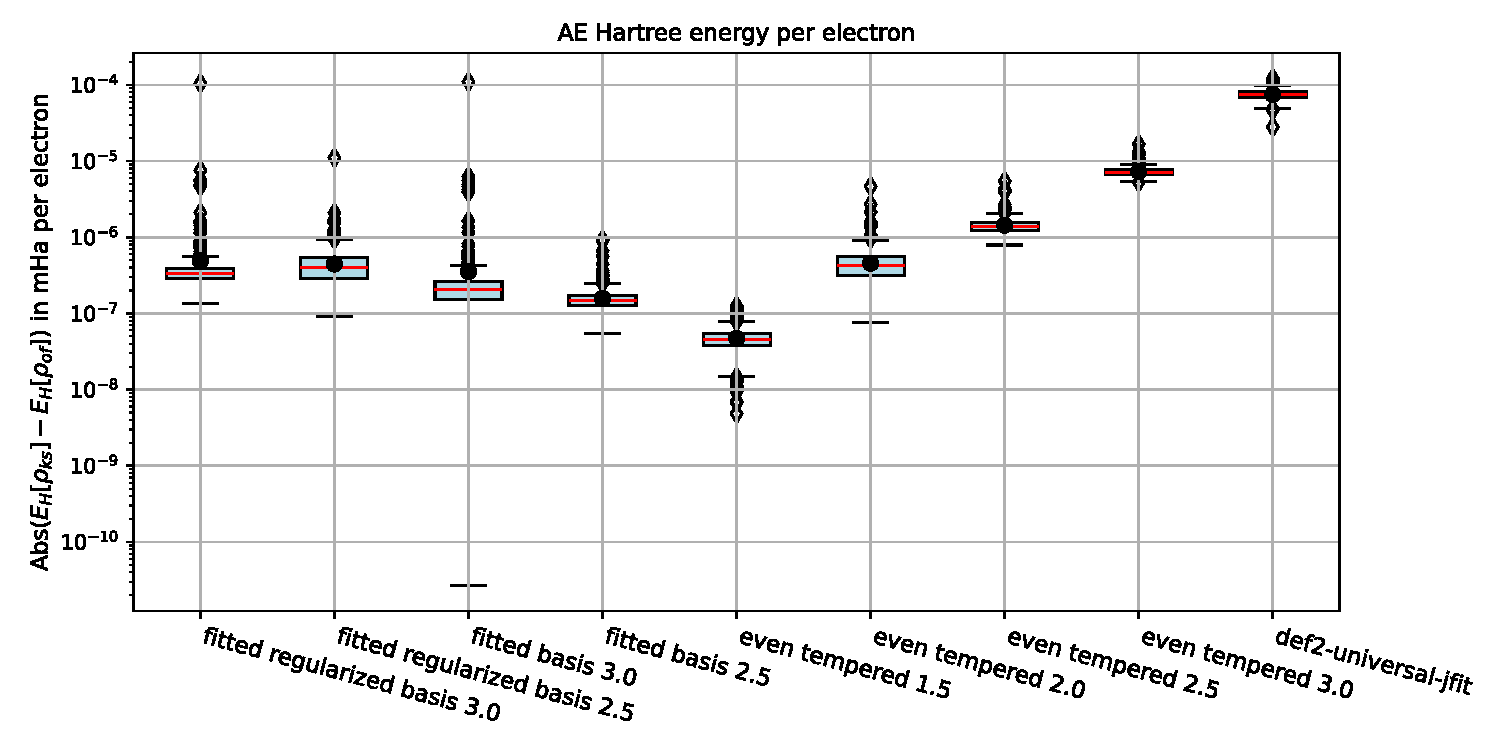
\includegraphics[width=0.75\textwidth]{chapters/results/results_images/AE_hartree_energy_on_hartree+external_MOFDFT_for_different_basis_sets}
    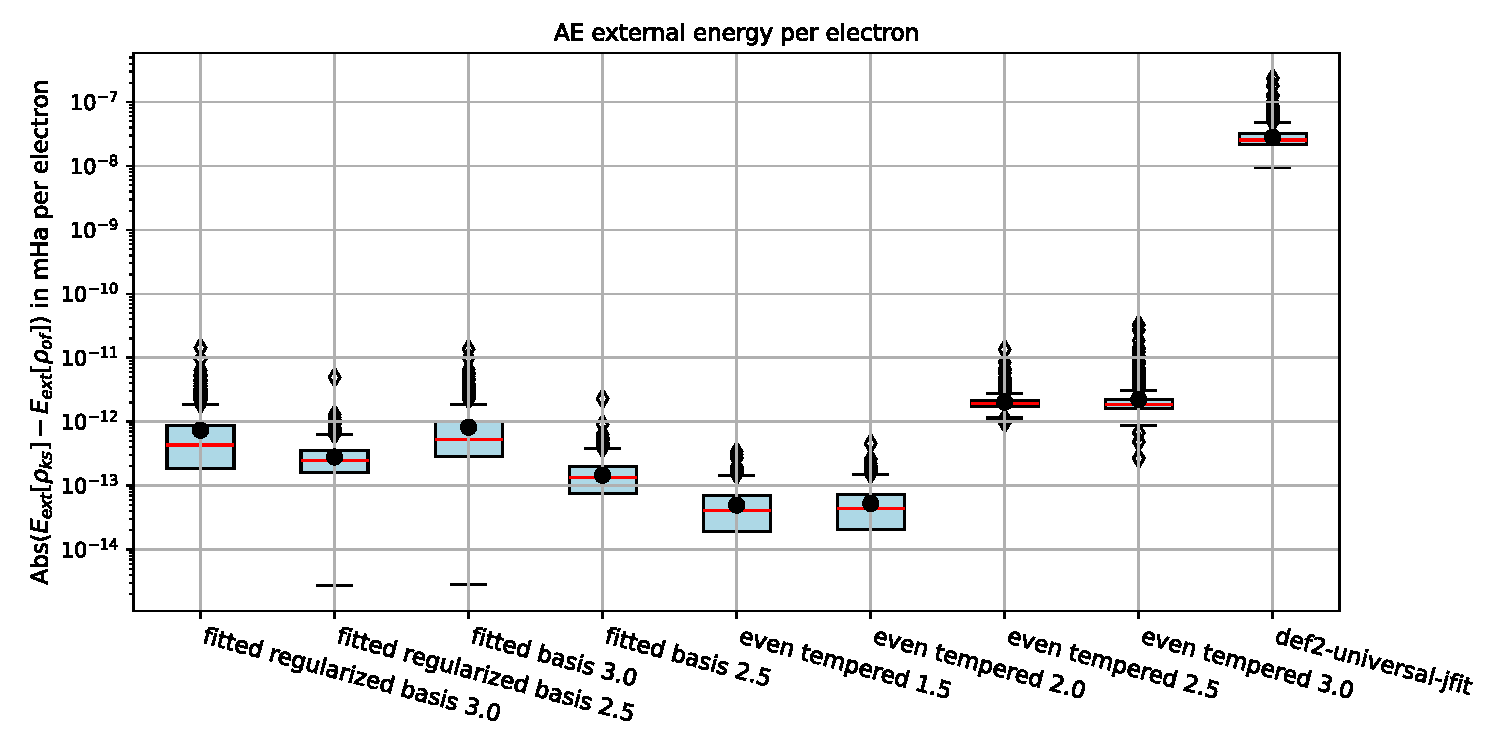
\includegraphics[width=0.75\textwidth]{chapters/results/results_images/AE_ext_energy_on_hartree+external_MOFDFT_for_different_basis_sets}
    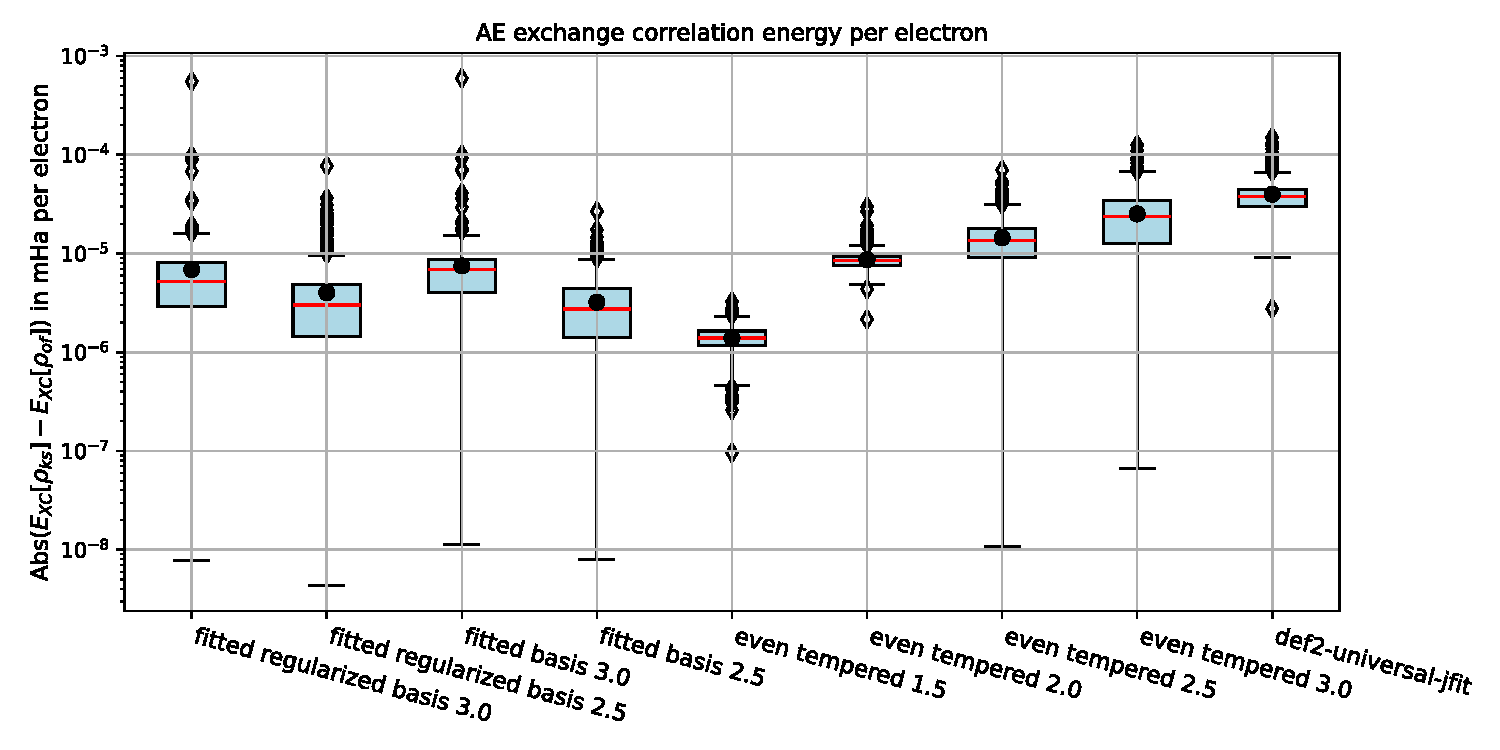
\includegraphics[width=0.75\textwidth]{chapters/results/results_images/AE_xc_energy_on_hartree+external_MOFDFT_for_different_basis_sets}
    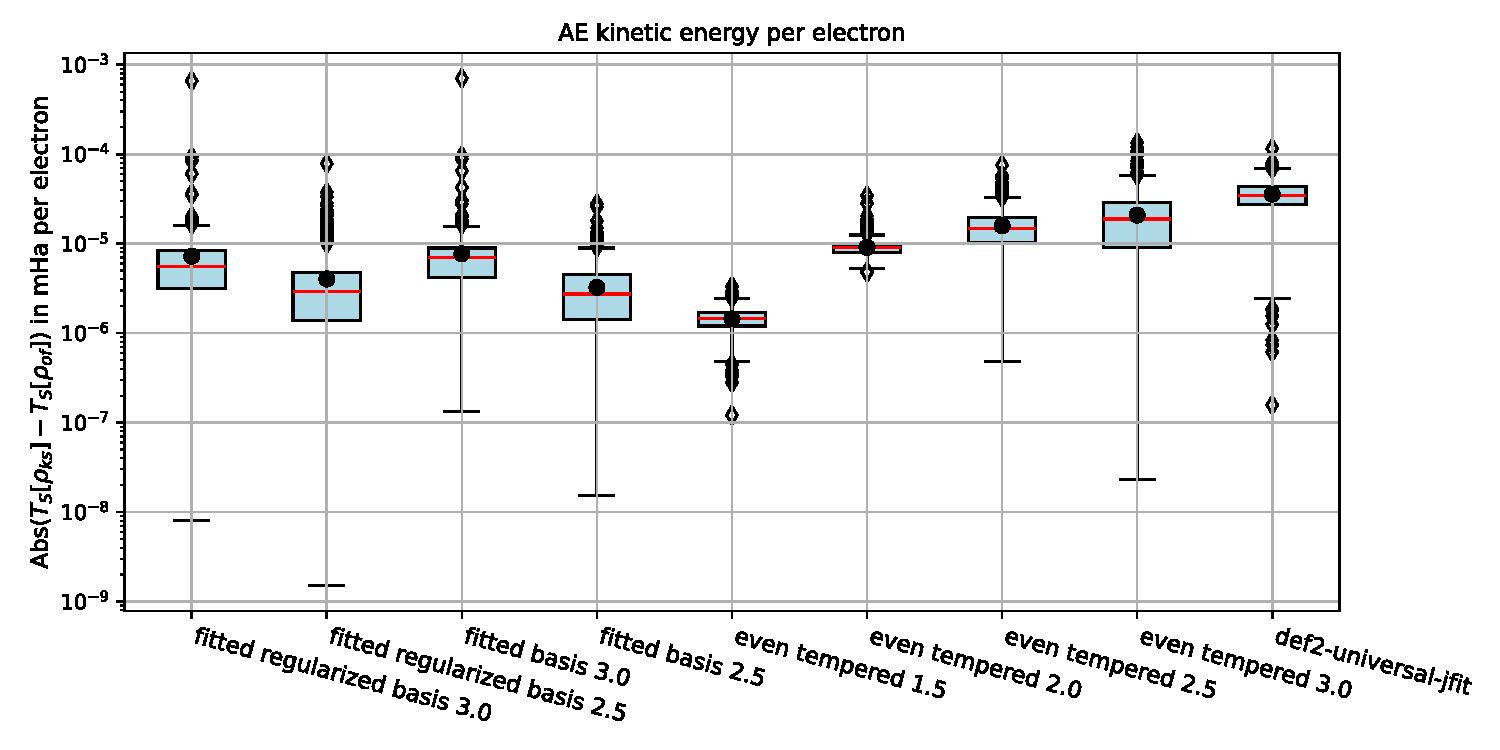
\includegraphics[width=0.75\textwidth]{chapters/results/results_images/AE_kin_energy_on_hartree+external_MOFDFT_for_different_basis_sets}
    \caption{Boxplots(\ref{boxplots}) of the AE for the different energies on the fitted basis sets averaged over the first 1000 molecules of QM9} \label{fig:AE_energies_basis_sets}
\end{figure}
\begin{figure}
    \centering
        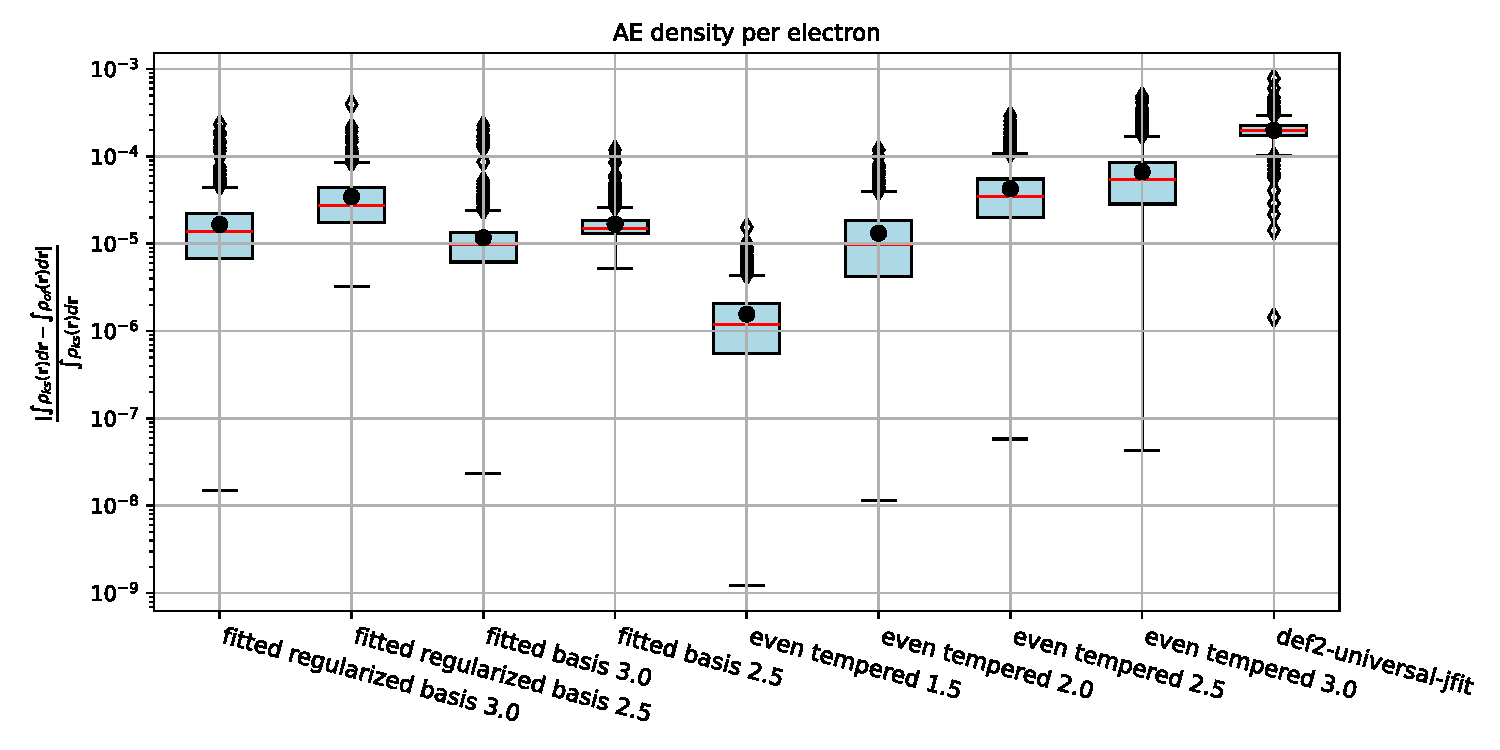
\includegraphics[width=0.75\textwidth]{chapters/results/results_images/AE_density_on_hartree+external_MOFDFT_for_different_basis_sets}
    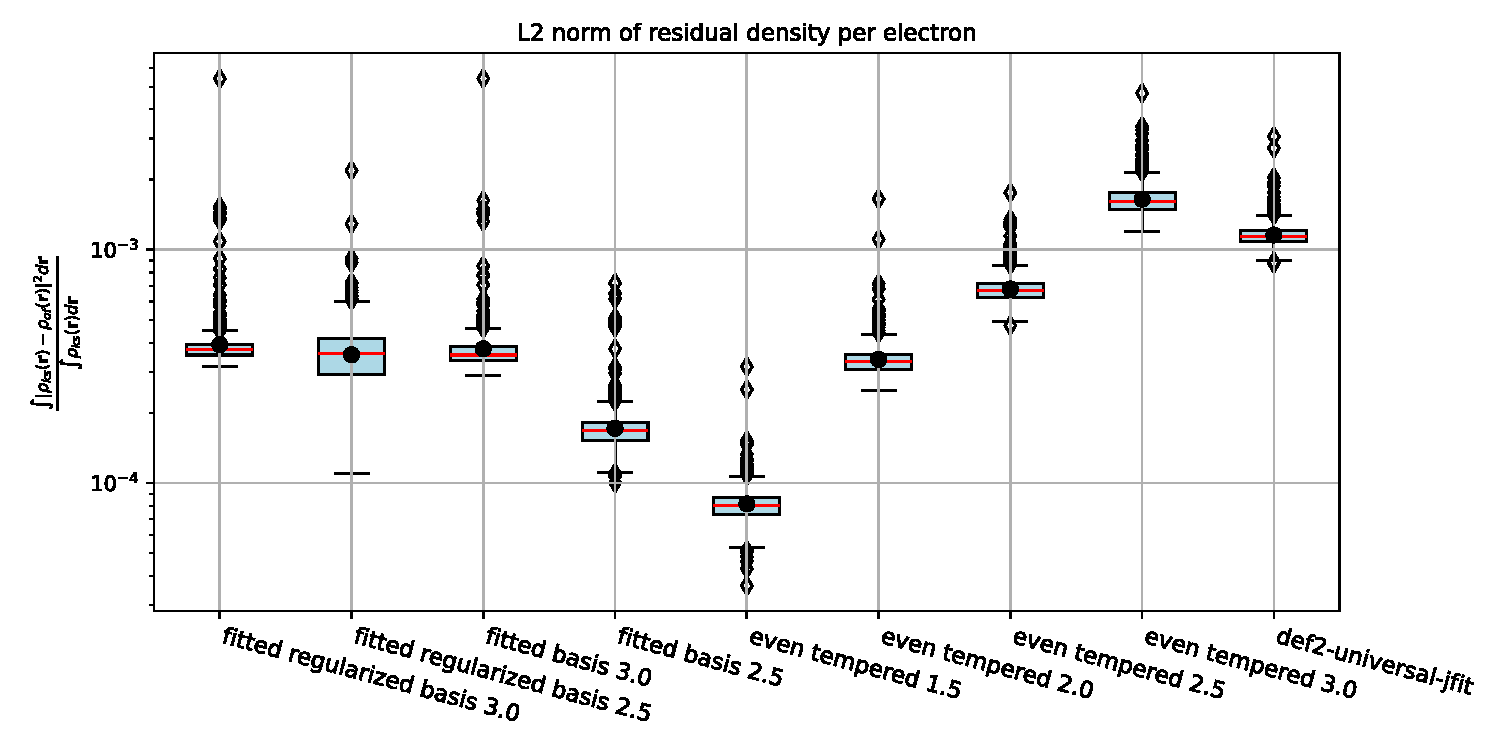
\includegraphics[width=0.75\textwidth]{chapters/results/results_images/L2_residual_densities_on_hartree+external_MOFDFT_for_different_basis_sets}
    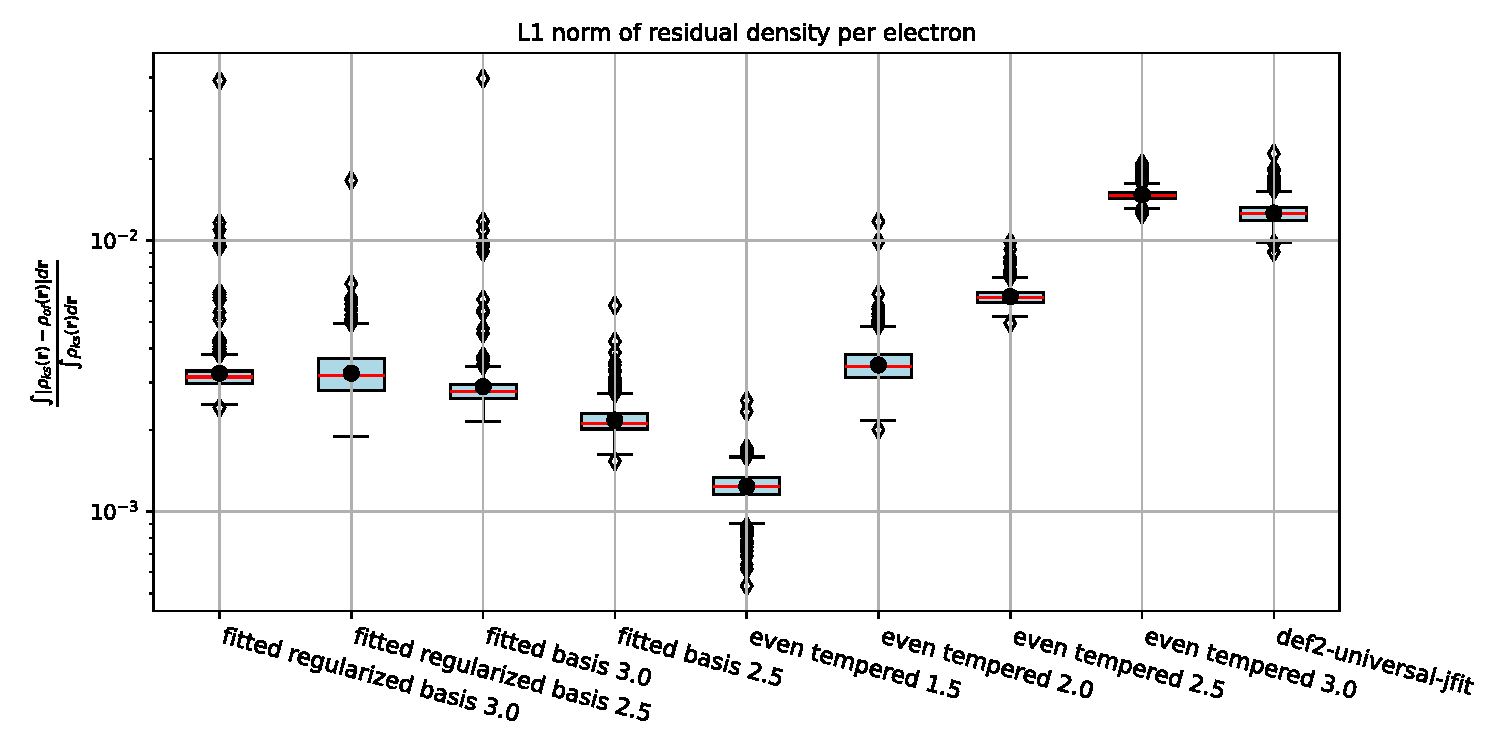
\includegraphics[width=0.75\textwidth]{chapters/results/results_images/L1_residual_densities_on_hartree+external_MOFDFT_for_different_basis_sets}
    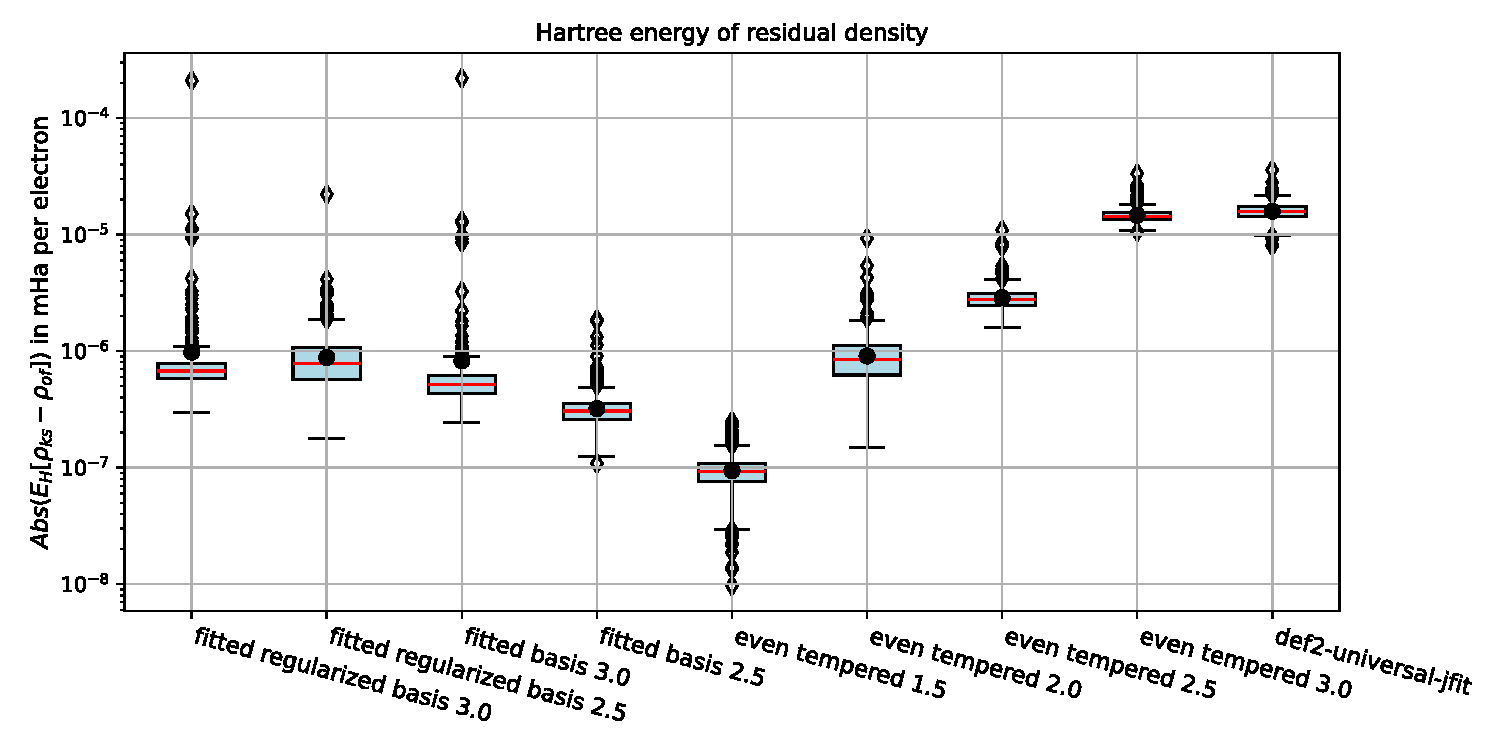
\includegraphics[width=0.75\textwidth]{chapters/results/results_images/L2_residual_hartree_on_hartree+external_MOFDFT_for_different_basis_sets}
\caption{Boxplots(\ref{boxplots}) comparing the error in density fitting for the different basis sets over the first 1000 molecules of QM9} \label{fig:density_error_basis_sets}
\end{figure}
    \begin{figure}
    \centering
    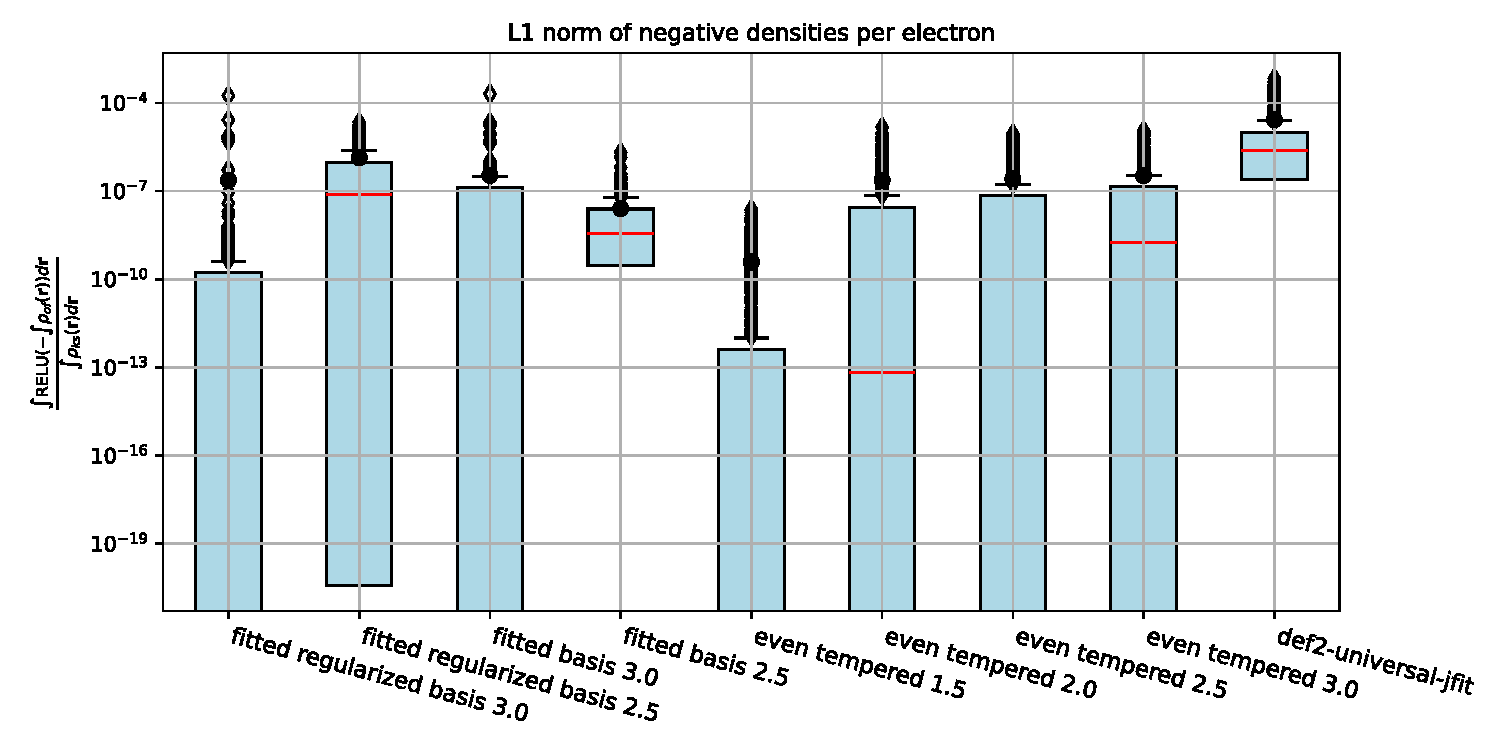
\includegraphics[width=0.9\textwidth]{chapters/results/results_images/L1_negative_densities_on_hartree+external_MOFDFT_for_different_basis_sets}
    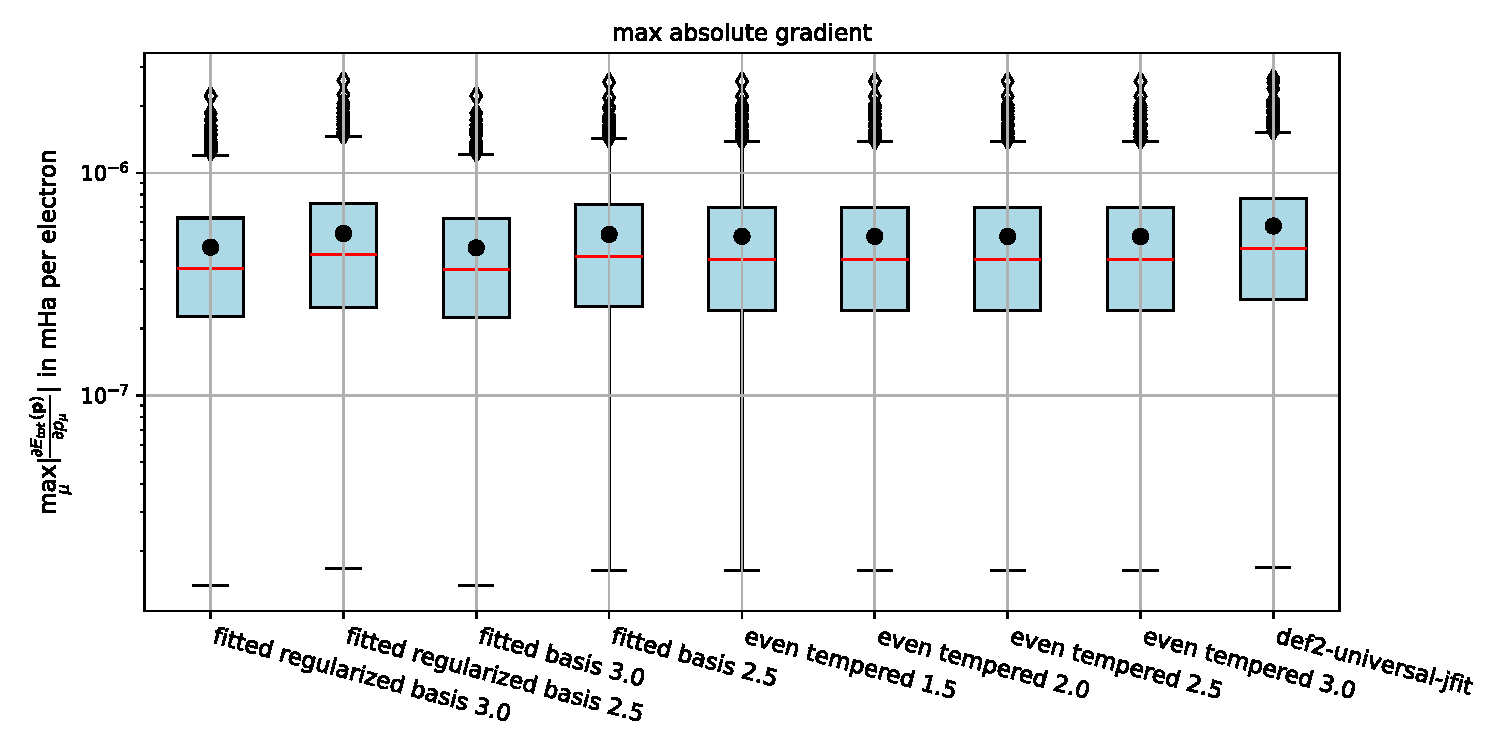
\includegraphics[width=0.9\textwidth]{chapters/results/results_images/max_abs_gradient_on_hartree+external_MOFDFT_for_different_basis_sets}
    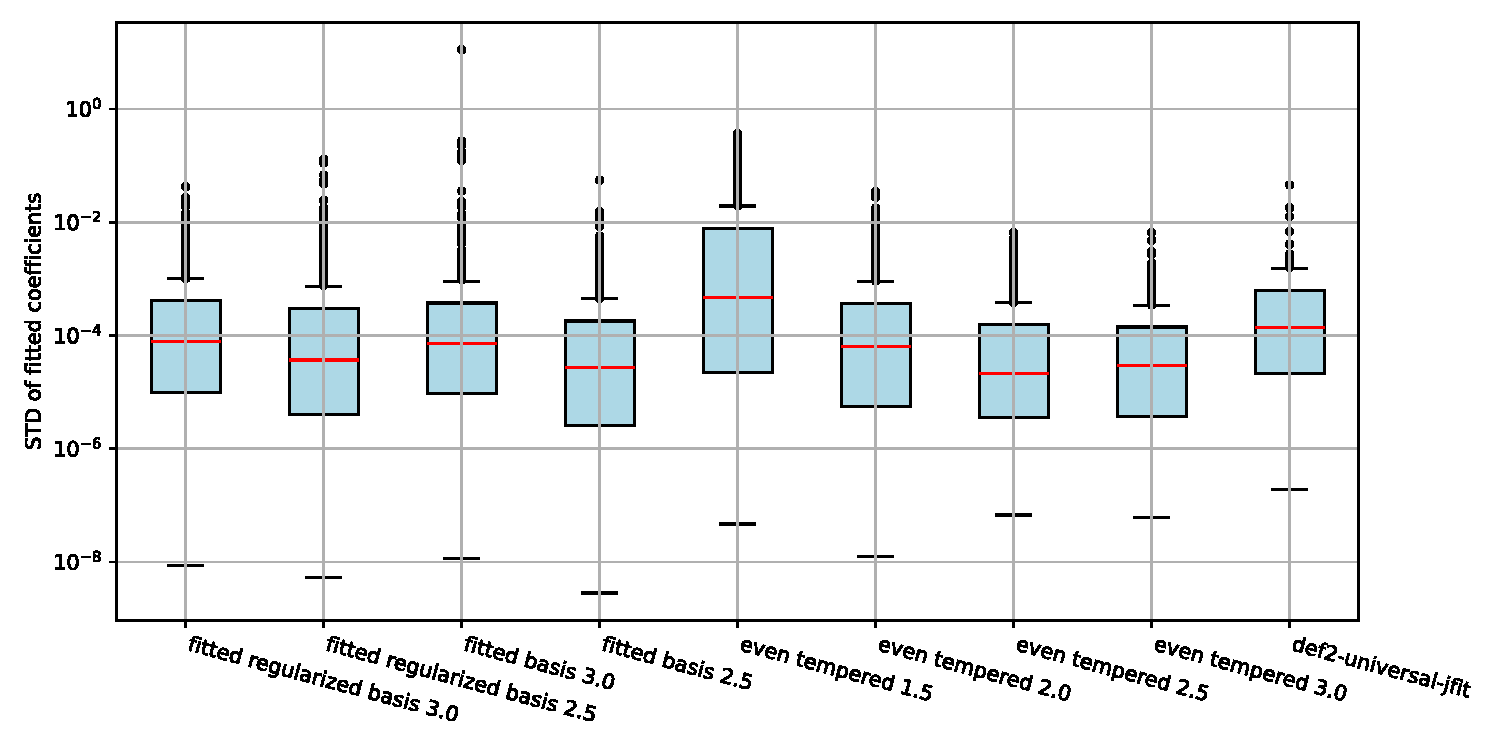
\includegraphics[width=0.9\textwidth]{chapters/results/results_images/var_basis_sets}
    \caption{Boxplots(\ref{boxplots}) analysing the different additional metrics for the fitted basis sets}
\end{figure}

\begin{figure}
    \centering
    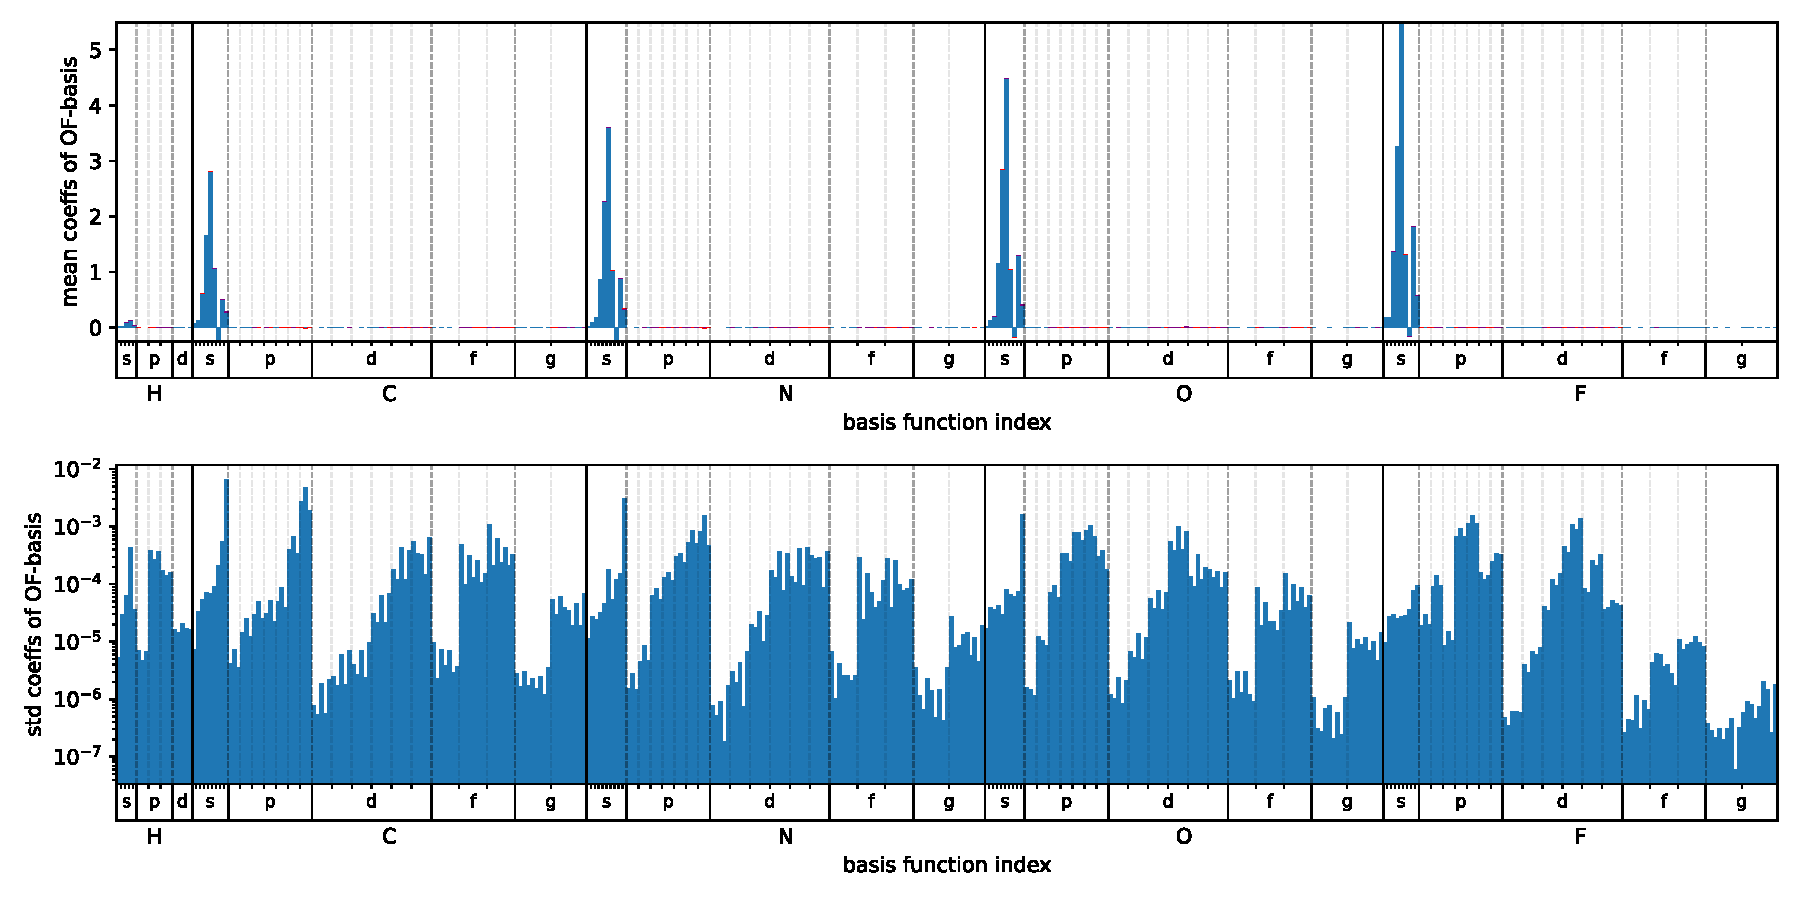
\includegraphics[width=0.9\textwidth]{chapters/results/results_images/var_coeffseven_tempered_3.0}
    \caption{The mean values(top) and the standart deviation(bottom) of the coefficients of an even tempered basis set with $\beta = 3.0$} \label{fig:var_coeffseven_tempered_3.0}
    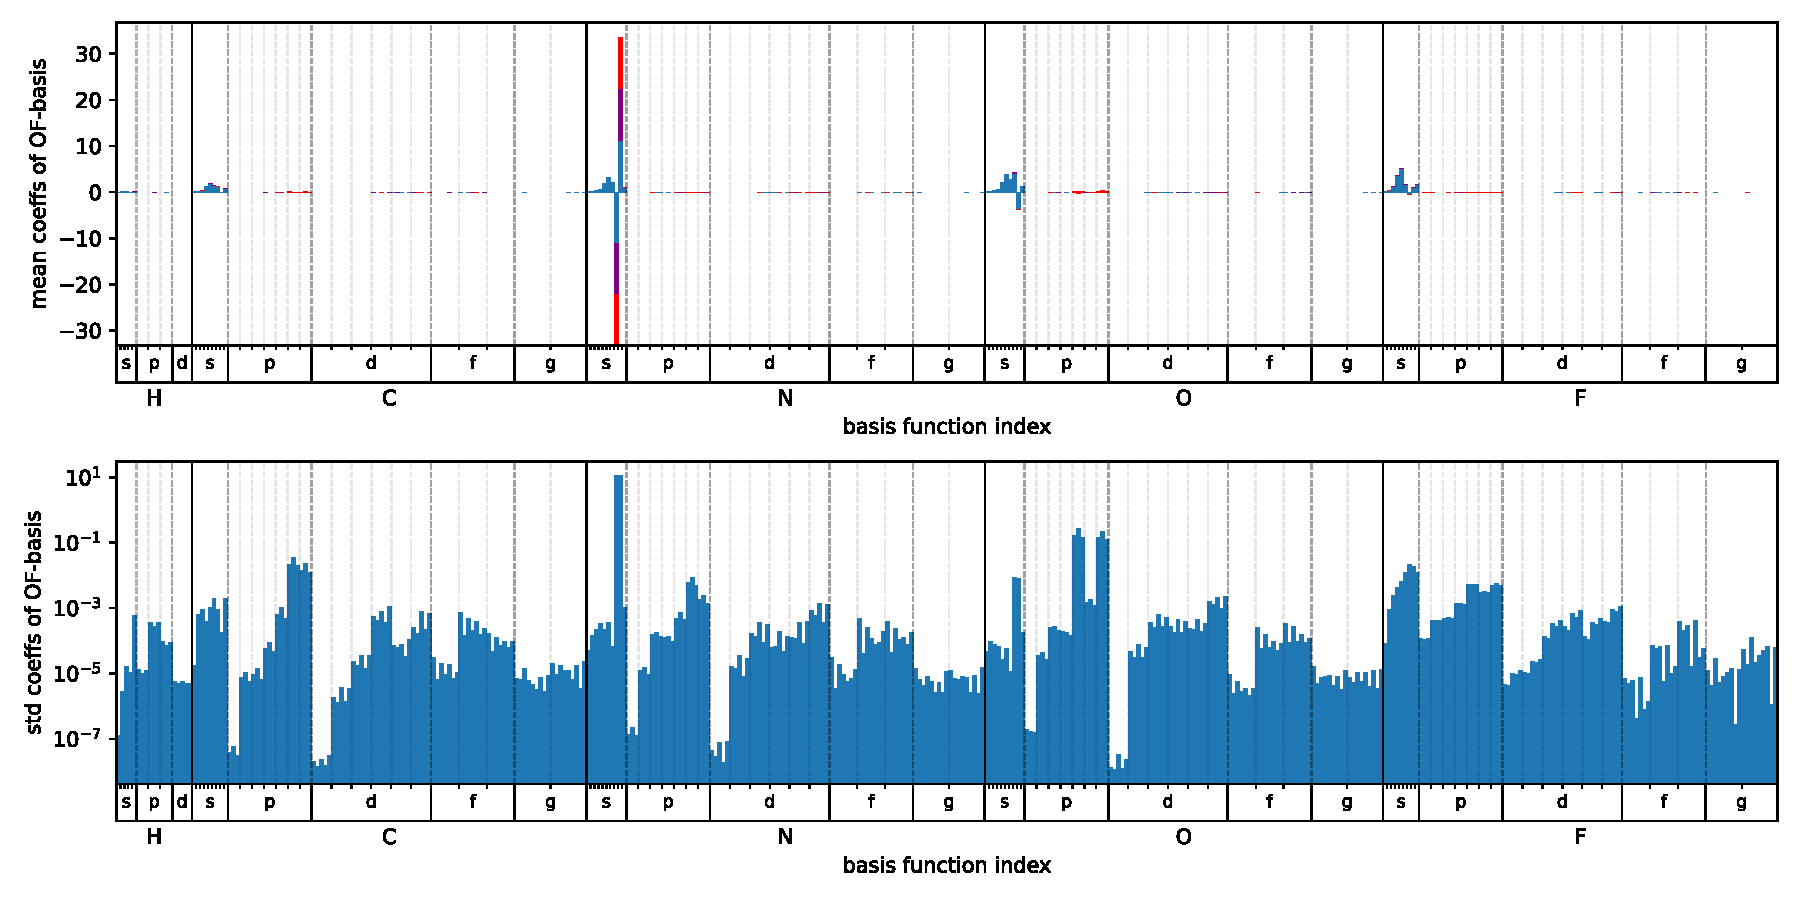
\includegraphics[width=0.9\textwidth]{chapters/results/results_images/var_coeffsfitted_basis_3.0}
        \caption{The mean values(top) and the standart deviation(bottom) of the coefficients of an basis set  fitted from even tempered with $\beta = 3.0$ without regularisation} \label{fig:var_coeffsfitted_basis_3.0}
    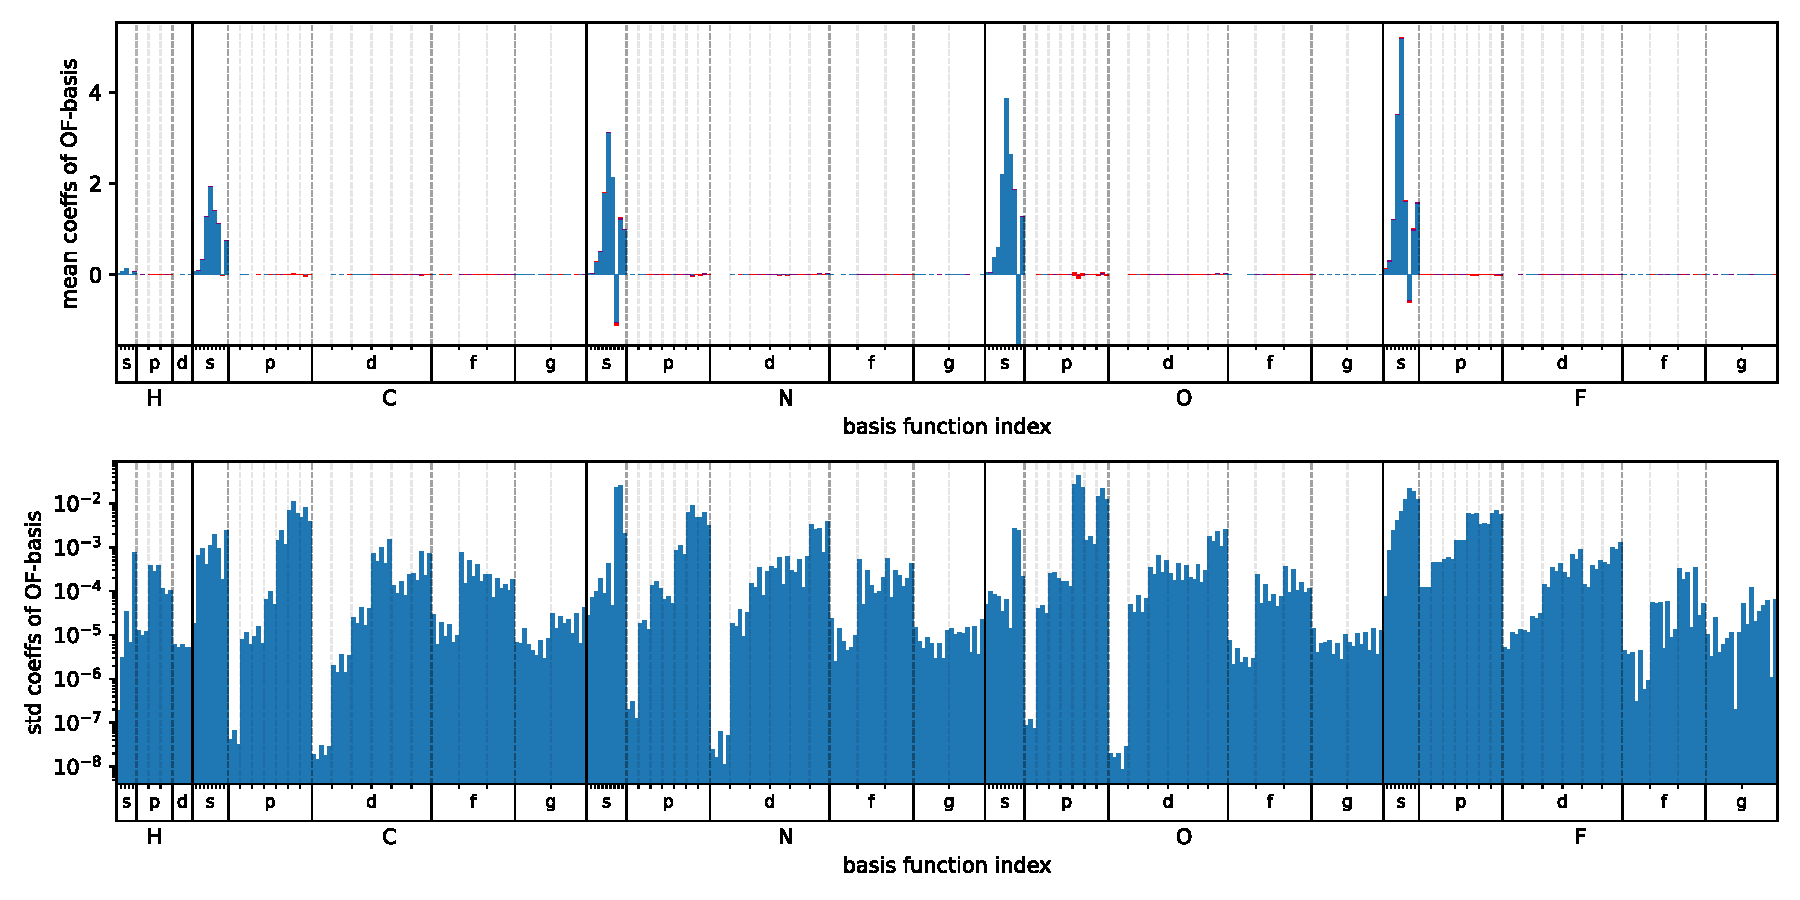
\includegraphics[width=0.9\textwidth]{chapters/results/results_images/var_coeffsfitted_regularized_basis_3.0}
        \caption{The mean values(top) and the standart deviation(bottom) of the coefficients of an basis set  fitted from even tempered with $\beta = 3.0$ after finetuning with regularisation} \label{fig:var_coeffsfitted_regularized_basis_3.0}
\end{figure}

 \begin{figure}
   \centering
   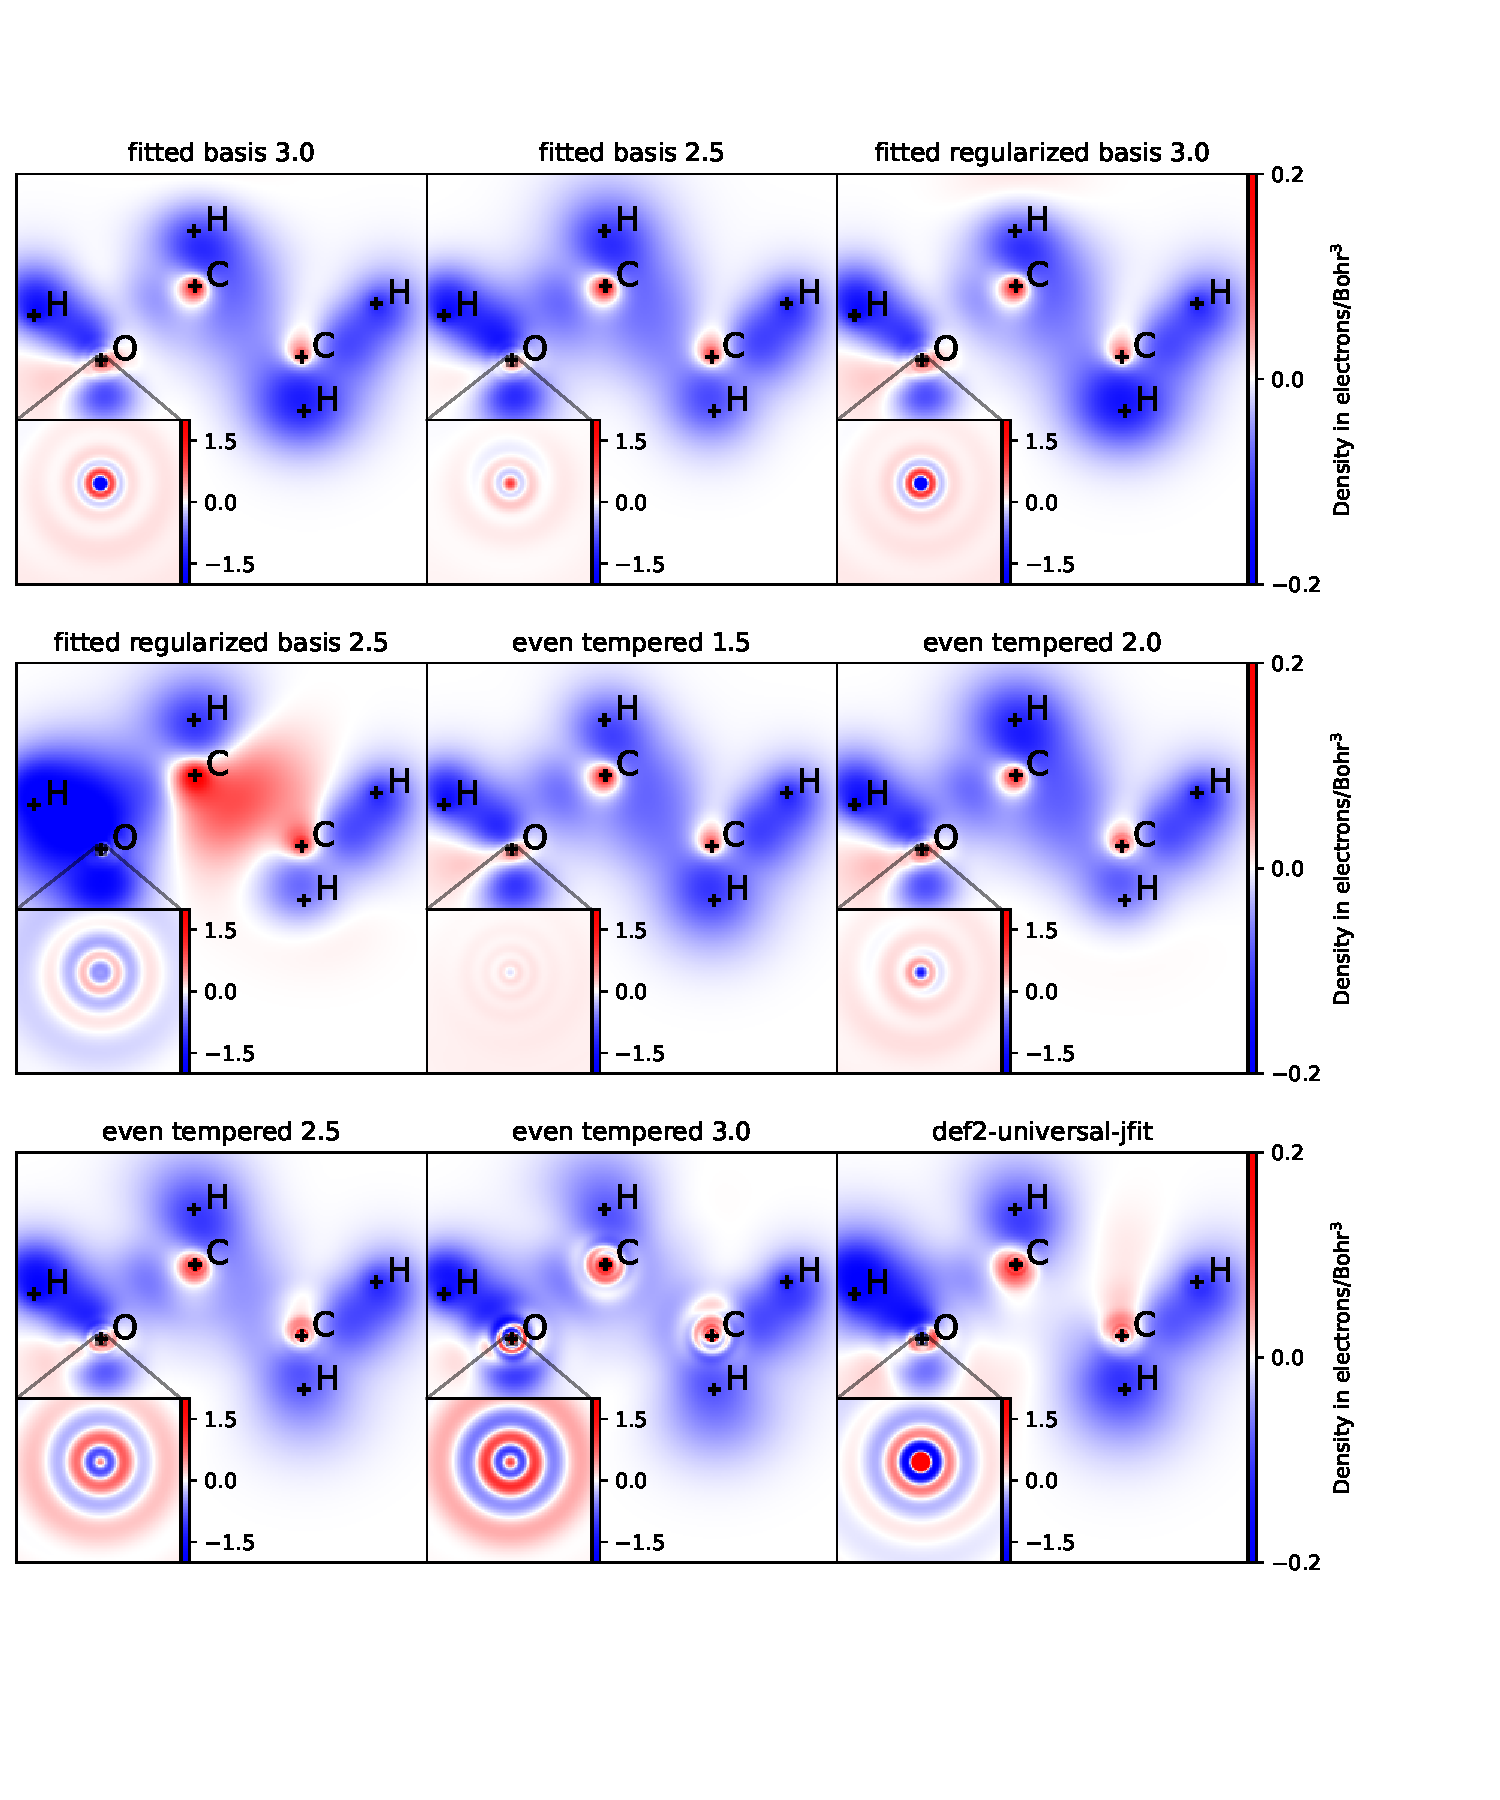
\includegraphics[width=1\textwidth]{chapters/results/results_images/basis_set_slices.pdf}
     \caption{Slices of the fitted density with density fitting method hartree+external Mofdft using different basis sets}
 \end{figure}



\begin{figure}
   \centering
   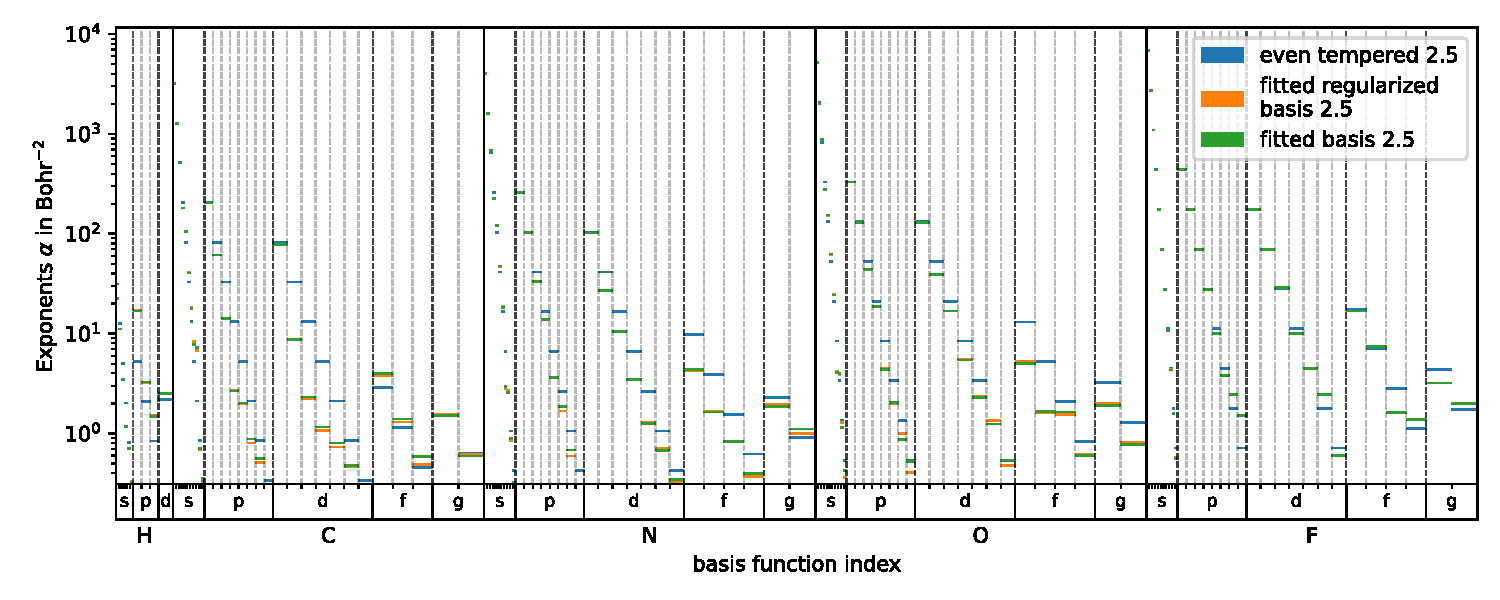
\includegraphics[width=0.6\textwidth]{chapters/results/results_images/basis_functions_with_size2.5}
   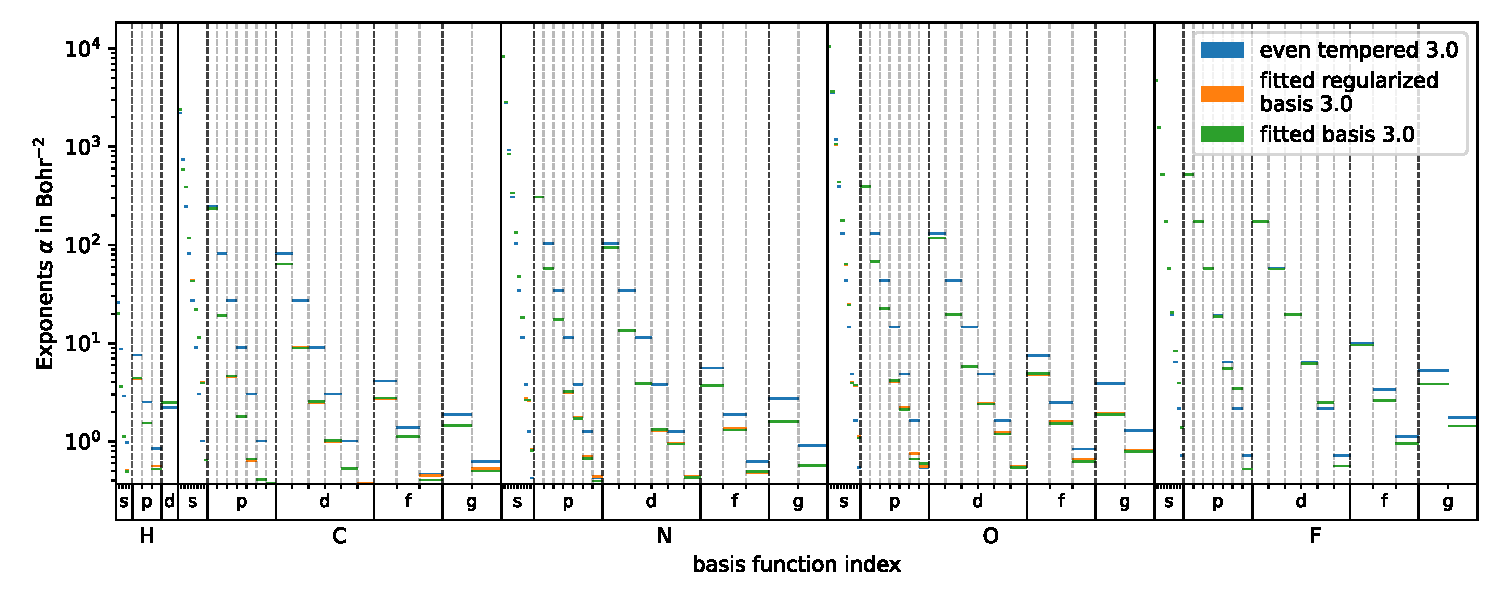
\includegraphics[width=0.6\textwidth]{chapters/results/results_images/basis_functions_with_size3.0}
    \caption{}
\end{figure}









\chapter{Adaptive basis functions for Kohn Sham Calculations}
As our differentiable basis set framework lets us differentiate through the whole basis set fitting procedere, we can choose to replace the constant basis functions that are commonly used in DFT calculation with adaptive ones which can adopt to the local chemical environment. First approaches in this direction were done by .... and recently with the rise of machine learing approches Linear fitted coefficient (...) and by a gaussian process predicted coefficients have been tried out. Adaptive exponents inside the Gaussian basis functions have been avoided so far as they require to differentiate through the integrals. But now owr framework allows us to to learn the coefficients and exponents used in dft calculations jointly. We mainly restrict our analysis to minimal basis sets, specificly the STO-3G\cite{STO-3G} minimal basis set, as they are exspected to profit the most from these improvements. We then use a small graph neural network, as described in \ref{Machine learning} to predict the exponents and coefficients of these Basis sets.
\section{Multi Step Pretraining}
As the differential basis functions are currently very slow and use a lot of vram compared to what is common in machine learing we cannot reach a very high number of iterations in learning. To compensate for this we using multiple pretraing procedere to improve the speed at which the neural network is learing. At first we let the network predict predict atomwise features, which don't require a evaluation of the differentiable integrals and can therefor be evaluated very quickly.
\subsection{Pretraining on atomwise properties}
We first evaluate the Neural network on atomwise properties to let it produce a kind of "physical intuition" before letting it work on the hard task of reliable predicting cefficients and expoenents for each atoms. For the features we borrow from the labels that have been produced for the orbital free model.
We predict the features by adding an extra linear output head at the last layer of the neural network. 
The following feature were predicted:
"atom_charges_all", "nuclear_energy_edges", "sum_forces", "n_electrons_atoms", "effective_charge_atoms", "kin_atoms",
"ext_atoms", "hartree_atoms", "xc_atoms", "tot_atoms"
\begin{enumerate}
    \item Atomic Number of each atom $Z_i$.\\
    \item Coulob potential from each neightboring Atom $-\sum\limits_{a\in \mathcal{N}(i)} \frac{Z_a}{|e_{i-a}|}$\\
    \item Sum of Coulomb forces acting on the current atom $\sum\limits_{a\in \mathcal{N}(i)} \frac{Z_aZ_i}{|e_{i-a}|^2}$\\
    \item Effective number of electrons $\sum_\mu \text{mask(i)}_\mu p_\mu w\mu$ \\
    \item Effective charge: Atomic Number - Effective number of electrons\\
    \item Integrated kinetic Gradient\\
    \item Integrated external energy of this atom\\
    \item Integrated hartree gradient\\
    \item Integrated xc gradient\\
    \item integrated total energy gradient\\
\end{enumerate}
where $\text{mask(i)}_\mu = \begin{array}{c} 1. \text{if} \omega_\mu(\mathbf{r}) \text{is centered on \mathbf{R_i}}\\0. \text{else} 
\end{array} $

\subsection{Orbitals Deltalearing to bigger basis set}
For the main traing step we train the basis set by fitting the orbitals produced by a largely bigger basis set 31-3g2fg? with the smaller basis set.
The derivation of this equation can be found in appendix... , it is identical to the common precedure of data whitening.
\begin{align}
    \text{Loss} &= \sum_{i,j} A^{-\frac{1}{2}} \langle\eta_\mu|\eta_\nu\rangle^{-1}_{\mu,nu} \langle\eta_\nu|\tilde\eta_\gamma) C_{i,\gamma}\\
    A_{i,j}&=C_{i,\sigma}\langle\eta_\sigma|\tilde\eta_\mu)\rangle \langle\eta_\mu|\eta_\nu\rangle^{-1}_{\mu,nu} \langle\eta_\nu|\tilde\eta_\gamma) C_{i,\gamma}\\
\end{align}







\begin{appendices}
    \chapter{Density Fitting Derivations}
    As intoduced in Chapter \ref{density_fitting_theory}
density fitting is ma method that attemps to reproduce the physical properties of a electron density produced by a set of orbitals by using a orbital free basis set.
In the following the different denisty fitting methods are introduced and compared.
\subsection{Metrics}
To evaluate the different density fitting methods the following metrics are used:
\begin{enumerate}
    \item Mean Absolute Error (MAE) of the Energies (Hartree, External, xc, kinetic)
    \item Mean Absolute Error (MAE) of the of the number of electrons $N = \int \rho(\mathbf{r}) d\mathbf{r}$
    \item The L2 Norm of the difference in densities $\text{L2}[\rho-\rho'] = \sqrt{\int (\rho(\mathbf{r})-\rho'(\mathbf{r}))^2} d\mathbf{r}$
    \item The L1 Norm of the difference in densities $\text{L1}[\rho-\rho'] = \int |\rho(\mathbf{r})-\rho'(\mathbf{r})| d\mathbf{r}$
    \item The Gradient of the total energy at the ground state (Interesting for convergence)
    \item The L1 Norm of negative values in the fitted density $\text{L1}[\rho'] = \int \text{RELU}(-\rho'(\mathbf{r})) d\mathbf{r}$
    \item The Hartree energy of the residual density $\text{Hartree}[\rho-\rho'] = \int \int \frac{(\rho(\mathbf{r})-\rho'(\mathbf{r}))(\rho(\mathbf{r'})-\rho'(\mathbf{r'}))}{|\mathbf{r}-\mathbf{r'}|}d\mathbf{r}d\mathbf{r'}$
    \item Stability of the fitted density coefficients (std of the coefficients)
\end{enumerate}
\subsection{Density fitting methods}
Here the different density fitting methods which were considert are introduced and compared.
The derivation are include in Appendix \ref{appendix:density_fitting}
\subsubsection{Overlap Density fitting}
\begin{align}
        \mathcal{L}(\mathbf{p}) &= \mathbf{p} W \mathbf{p} - 2 \mathbf{p}\bar { L} \bar\Gamma + \bar\Gamma \mathbf{D}\bar\Gamma
\end{align}

\subsubsection{Hartree Density fitting}
Minimizes the following metric:
\begin{align}
        \mathcal{L}(\mathbf{p}) &= \mathbf{p} \tilde{W} \mathbf{p} - 2 \mathbf{p}\bar {\tilde L} \bar\Gamma + \bar\Gamma \tilde{\mathbf{D}}\bar\Gamma
\end{align}
Which results in the following formula for the fitted density coefficients:
\begin{align}
    \mathbf{p}&=\tilde{W}^{-1}\bar {\tilde L} \bar\Gamma\\
\end{align}


\subsubsection{Hartree+External Density Fitting}
\begin{align}
        \mathcal{L}(\mathbf{p}) &= \mathbf{p} \tilde{W} \mathbf{p} - 2 \mathbf{p}\bar {\tilde L} \bar\Gamma + \bar\Gamma \tilde{\mathbf{D}}\bar\Gamma + (\mathbf{p}\mathbf{v}_{ext}-\bar\Gamma \bar{V}_{ext})^2
\end{align}
\begin{align}
    A&:=\tilde{W}+\mathbf{v}_{ext}\mathbf{v}_{ext}^T\\
    \mathbf{p}&:=A^{-1}\left(\bar {\tilde L}+\mathbf{v}_{ext}\bar{V}_{ext}\right) \bar\Gamma\\
\end{align}

\subsubsection{Hartree+External Density Fitting MOFDFT-Version}
\begin{align}
\mathcal{L}(\mathbf{p}) &= \mathbf{p} \tilde{W} \mathbf{p} - 2 \mathbf{p}\bar {\tilde L} \bar\Gamma + \bar\Gamma \tilde{\mathbf{D}}\bar\Gamma + (\mathbf{p}\mathbf{v}_{ext}-\bar\Gamma \bar{V}_{ext})^2\\
&\left(\begin{array}{c}\tilde{W}\\v_{ext}^T\end{array}\right) \mathbf{p} =  \left(\begin{array}{c}\tilde{L} \bar{\Gamma} \\ \bar{\Gamma}\bar{V}_{ext}\end{array}\right)
\end{align}


\subsubsection{Hartree+External Density Fitting with enforced electron number}
\begin{align}
    \mathcal{L}(\mathbf{p},\mu) &= \mathbf{p} \tilde{W} \mathbf{p} - 2 \mathbf{p}\bar {\tilde L} \bar\Gamma + (\mathbf{p}\mathbf{v}_{ext}-\bar\Gamma \bar{V}_{ext})^2+\mu(\mathbf{p}\mathbf{w}-\bar\Gamma\bar S)\\
    A^{-1}\left(\bar {\tilde L} + \mathbf{v}_{ext} \bar{V}_{ext}- \mathbf{w}\frac{\mathbf{w}A^{-1}\bar {\tilde L} +\mathbf{w}A^{-1}\mathbf{v}_{ext} \bar{V}_{ext}-\bar S}{\mathbf{w}A^{-1}\mathbf{w}}\right)\bar\Gamma\\
\end{align}



\subsubsection{Hartree Density Fitting with enforced electron number and enforced external energy}
\begin{align}
    \mathcal{L}(\mathbf{p},\mu,\nu) &= \mathbf{p} \tilde{W} \mathbf{p} - 2 \mathbf{p}\bar {\tilde L} \bar\Gamma + \nu(\mathbf{p}\mathbf{v}_{ext}-\bar\Gamma \bar{V}_{ext})+\mu(\mathbf{p}\mathbf{w}-\bar\Gamma\bar S)\\
\end{align}


\subsubsection{Hartree+External Density Fitting MOFDFT-Version with soft enforced electron number}
\begin{align}
    \mathcal{L}(\mathbf{p}) &= \mathbf{p} \tilde{W} \mathbf{p} - 2 \mathbf{p}\bar {\tilde L} \bar\Gamma + \bar\Gamma \tilde{\mathbf{D}}\bar\Gamma + (\mathbf{p}\mathbf{v}_{ext}-\bar\Gamma \bar{V}_{ext})^2 + (\mathbf{p}\mathbf{w}-\bar\Gamma \bar{S})^2
\end{align}
\begin{align}
    \left(\begin{array}{c}\tilde{W}\\\mathbf{v}_{ext}^T\\\mathbf{w}^T\end{array}\right) \mathbf{p} =  \left(\begin{array}{c}\tilde{L} \bar{\Gamma} \\ \bar{\Gamma}\bar{V}_{ext}\\\bar S\bar \Gamma\end{array}\right)
\end{align}


\subsubsection{Hartree+External Density Fitting MOFDFT-Version with hard enforced electron number}
\begin{align}
    \mathcal{L}(\mathbf{p}) &= \left\lVert\left(\begin{array}{c}\tilde{W}\\v_{ext}^T\end{array}\right) \mathbf{p} - \left(\begin{array}{c}\tilde{L} \bar{\Gamma} \\ \bar{\Gamma}\bar{V}_{ext}\end{array}\right)\right\rVert^2 + \lambda (\mathbf{w}\mathbf{p}-N)
\end{align}



\subsubsection{Overlap Density fitting with enforced electron number}
\begin{align}
    \mathcal{L}(\mathbf{p},\mu) &= \mathbf{p} \tilde{W} \mathbf{p} - 2 \mathbf{p}\bar {\tilde L} \bar\Gamma + (\mathbf{p}\mathbf{v}_{ext}-\bar\Gamma \bar{V}_{ext})^2+\mu(\mathbf{p}\mathbf{w}-\bar\Gamma\bar S)\\
    A^{-1}\left(\bar {\tilde L} + \mathbf{v}_{ext} \bar{V}_{ext}- \mathbf{w}\frac{\mathbf{w}A^{-1}\bar {\tilde L} +\mathbf{w}A^{-1}\mathbf{v}_{ext} \bar{V}_{ext}-\bar S}{\mathbf{w}A^{-1}\mathbf{w}}\right)\bar\Gamma\\
\end{align}



\subsubsection{Overlap Density fitting with enforced electron number and enforced external energy}
\begin{align}
    \mathcal{L}(\mathbf{p},\mu,\nu) &= \mathbf{p} \tilde{W} \mathbf{p} - 2 \mathbf{p}\bar {\tilde L} \bar\Gamma + \nu(\mathbf{p}\mathbf{v}_{ext}-\bar\Gamma \bar{V}_{ext})+\mu(\mathbf{p}\mathbf{w}-\bar\Gamma\bar S)\\
\end{align}

The following plot shows the difference of the metrics evaluated on the first 1000 Molecules of QM9.

Insert plot here

A more detailed Table of the found falues for the different values can be found in the appendix\cite appendix.

\begin{figure}[h]
    \centering
    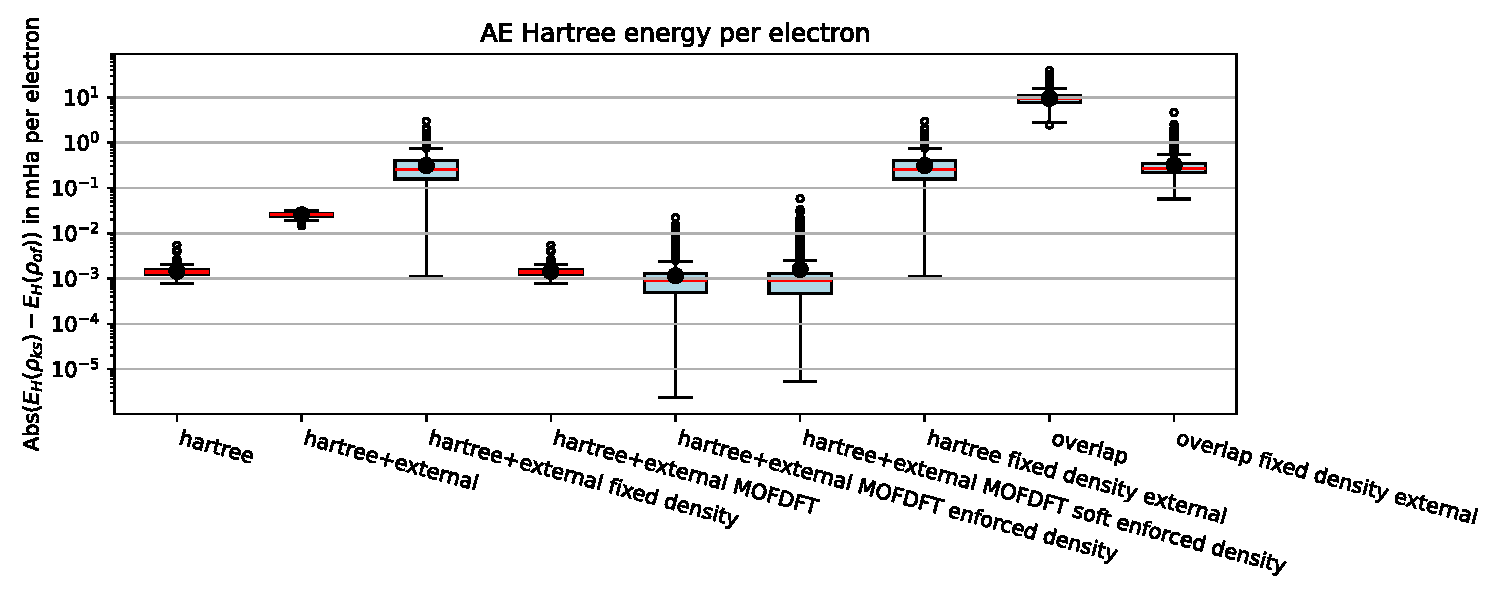
\includegraphics[width=0.5\textwidth]{chapters/results/results_images/AE_hartree_energy_on_even_tempered_2.5}
    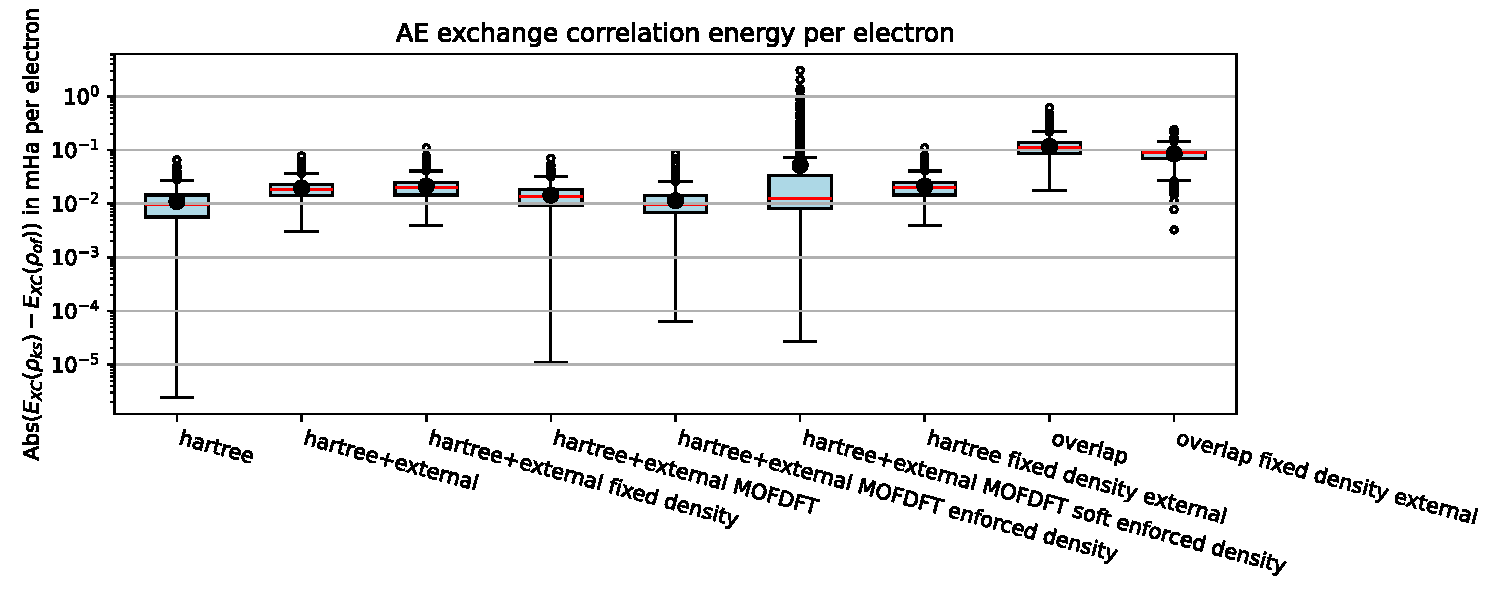
\includegraphics[width=.49\textwidth]{chapters/results/results_images/AE_xc_energy_on_even_tempered_2.5}
    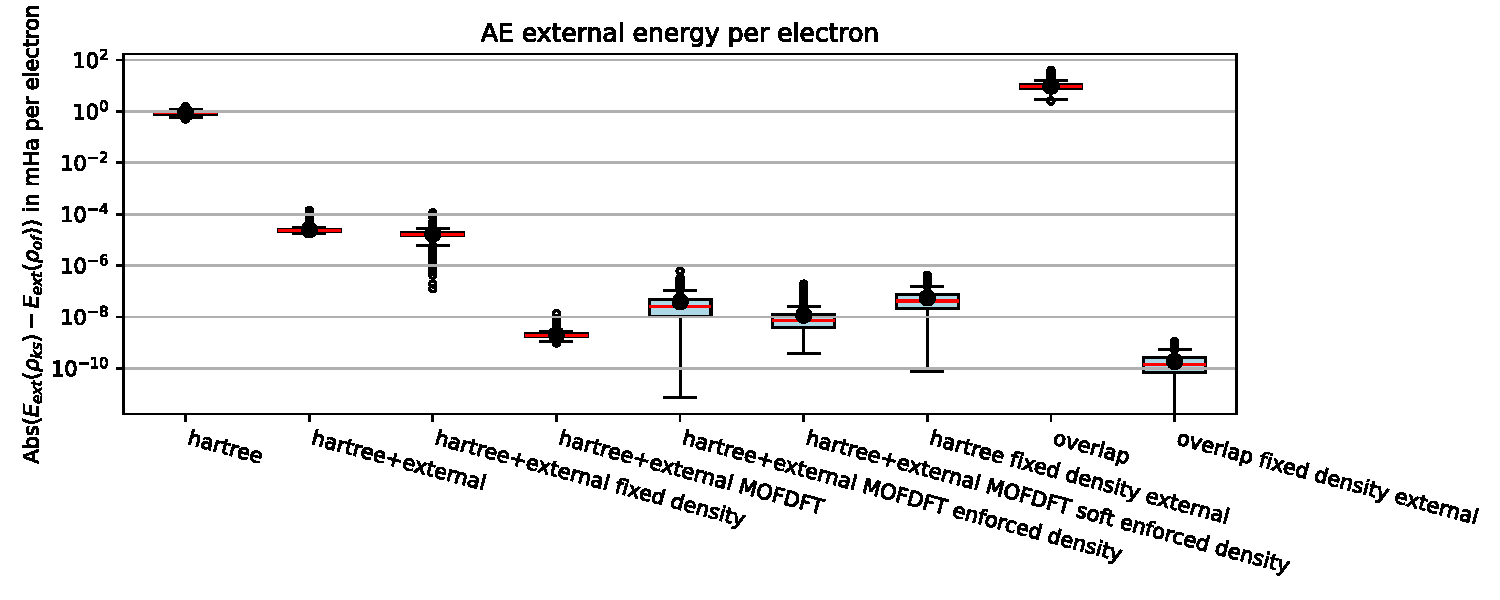
\includegraphics[width=.5\textwidth]{chapters/results/results_images/AE_ext_energy_on_even_tempered_2.5}
    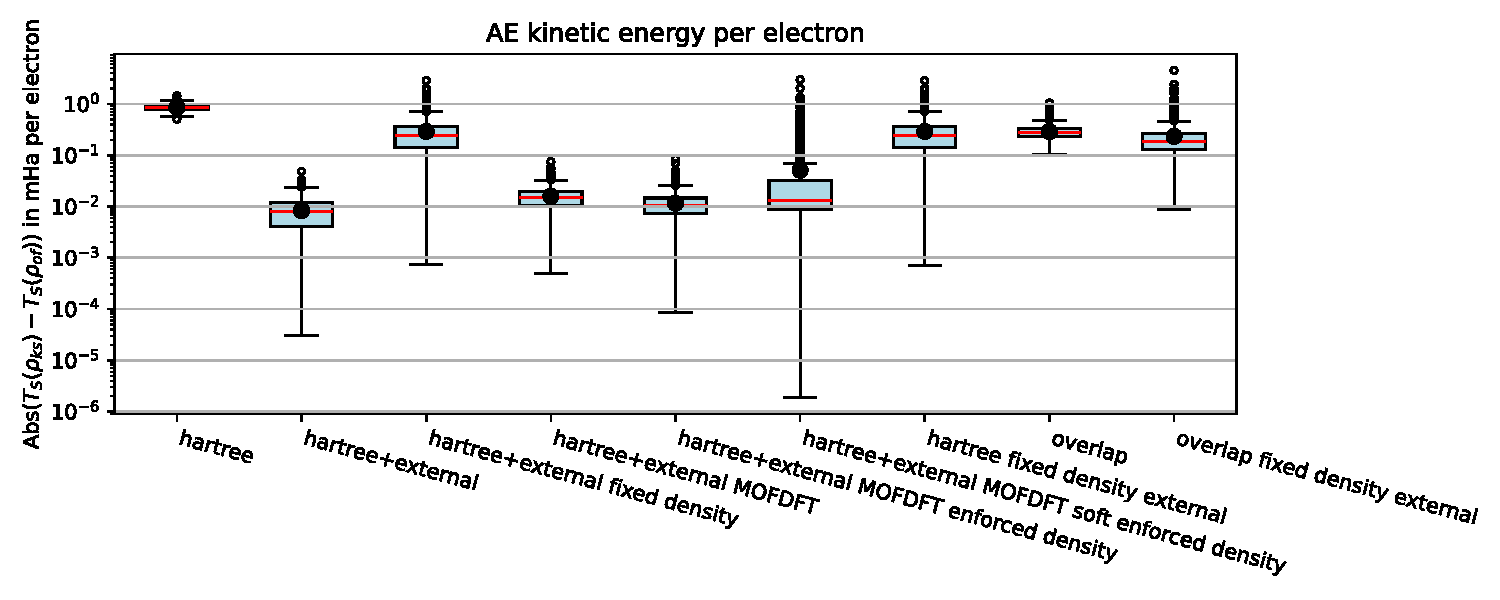
\includegraphics[width=.49\textwidth]{chapters/results/results_images/AE_kin_energy_on_even_tempered_2.5}
    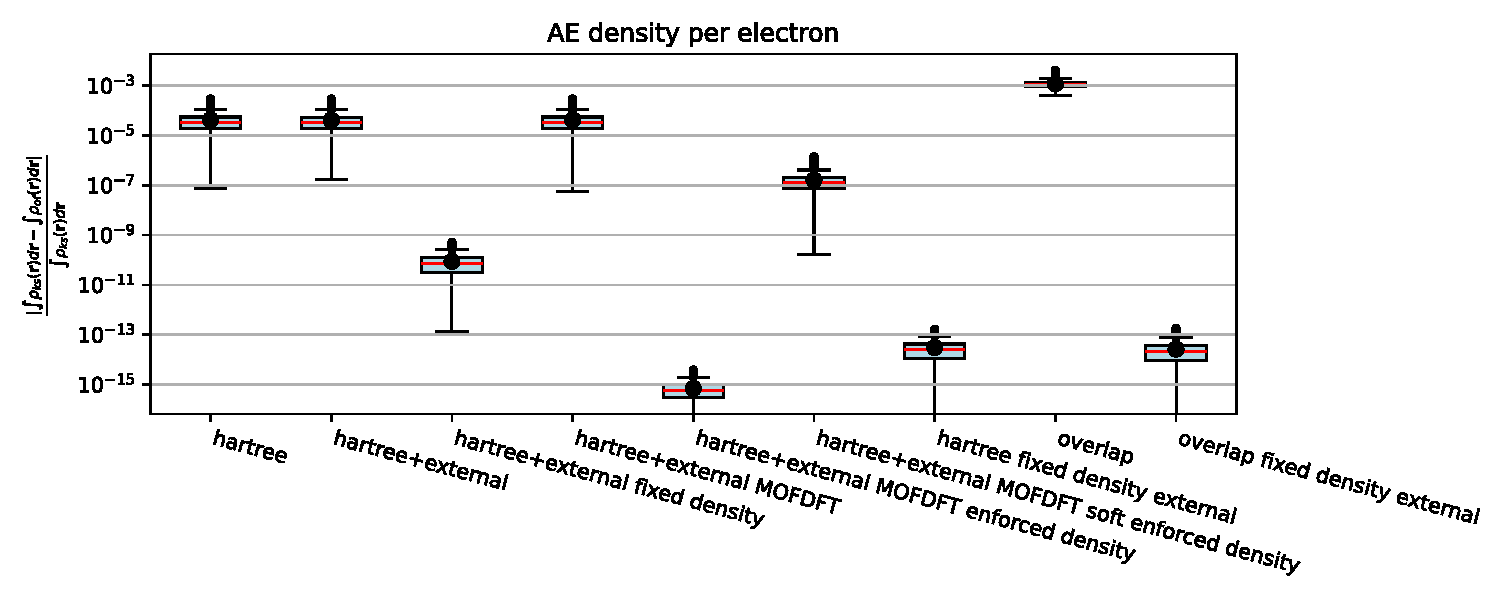
\includegraphics[width=.5\textwidth]{chapters/results/results_images/AE_density_on_even_tempered_2.5}
    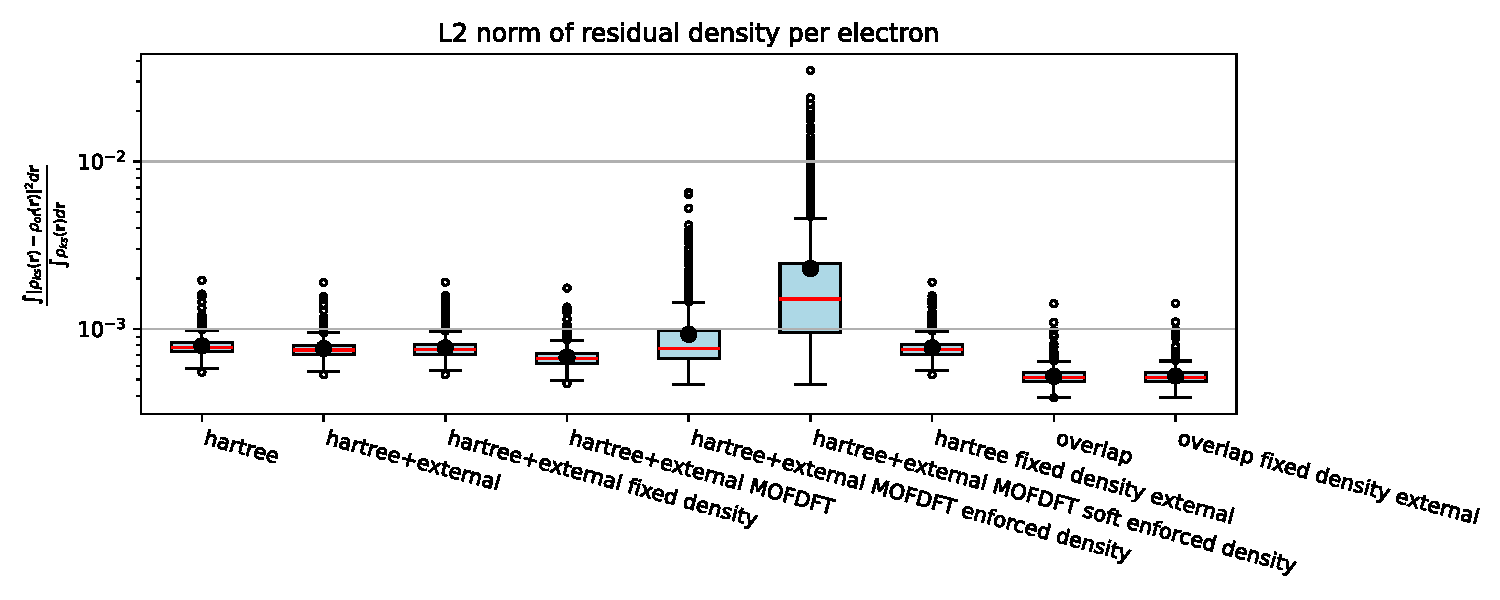
\includegraphics[width=0.49\textwidth]{chapters/results/results_images/L2_residual_densities_on_even_tempered_2.5}
    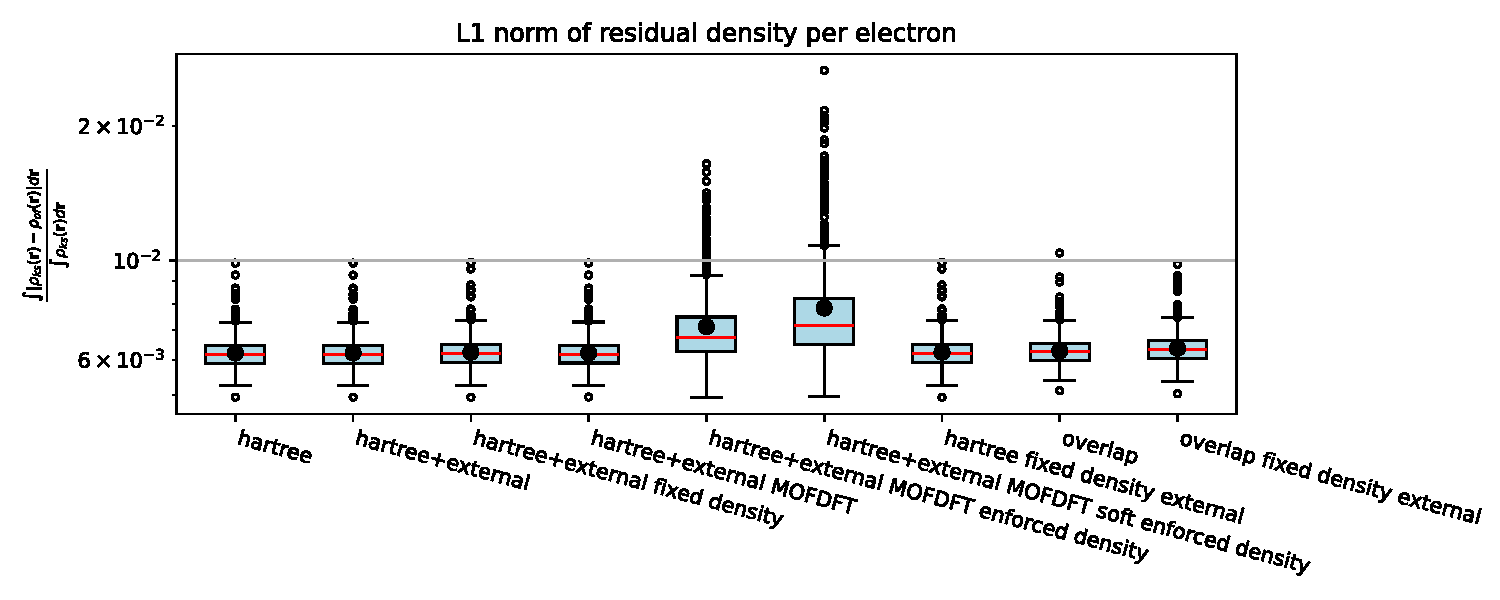
\includegraphics[width=0.5\textwidth]{chapters/results/results_images/L1_residual_densities_on_even_tempered_2.5}
    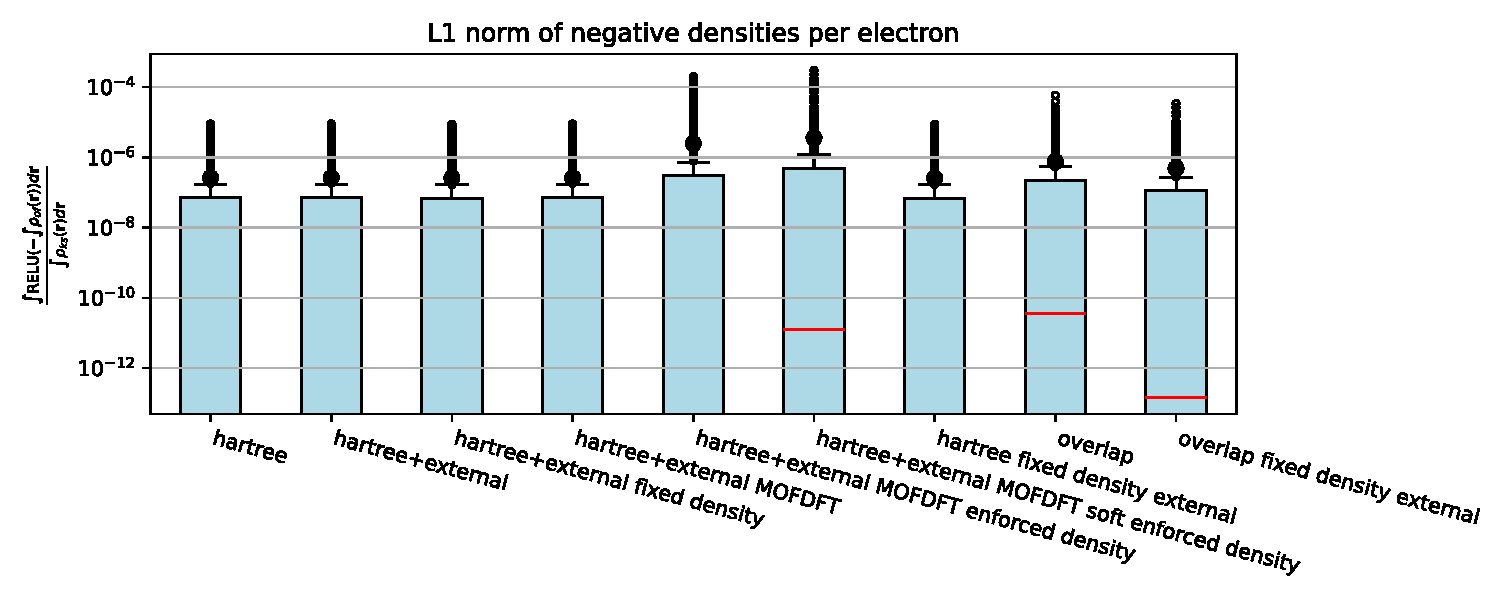
\includegraphics[width=0.49\textwidth]{chapters/results/results_images/L1_negative_densities_on_even_tempered_2.5}
    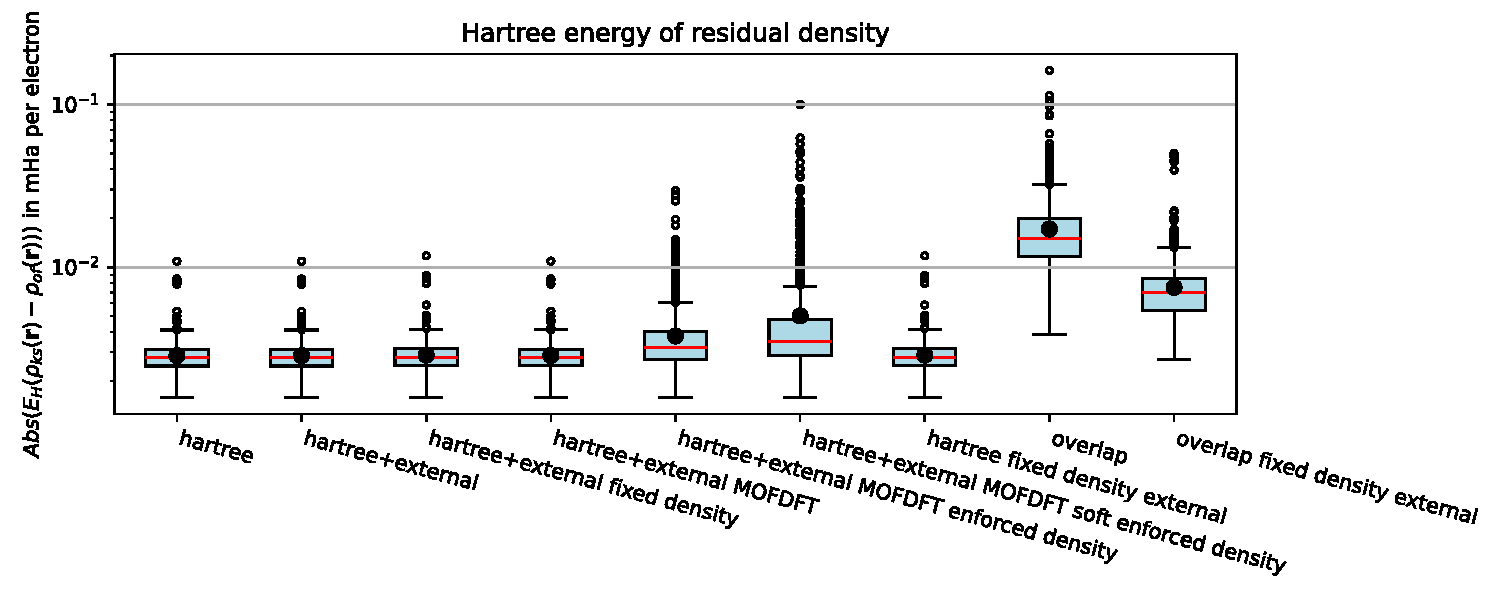
\includegraphics[width=0.5\textwidth]{chapters/results/results_images/L2_residual_hartree_on_even_tempered_2.5}
    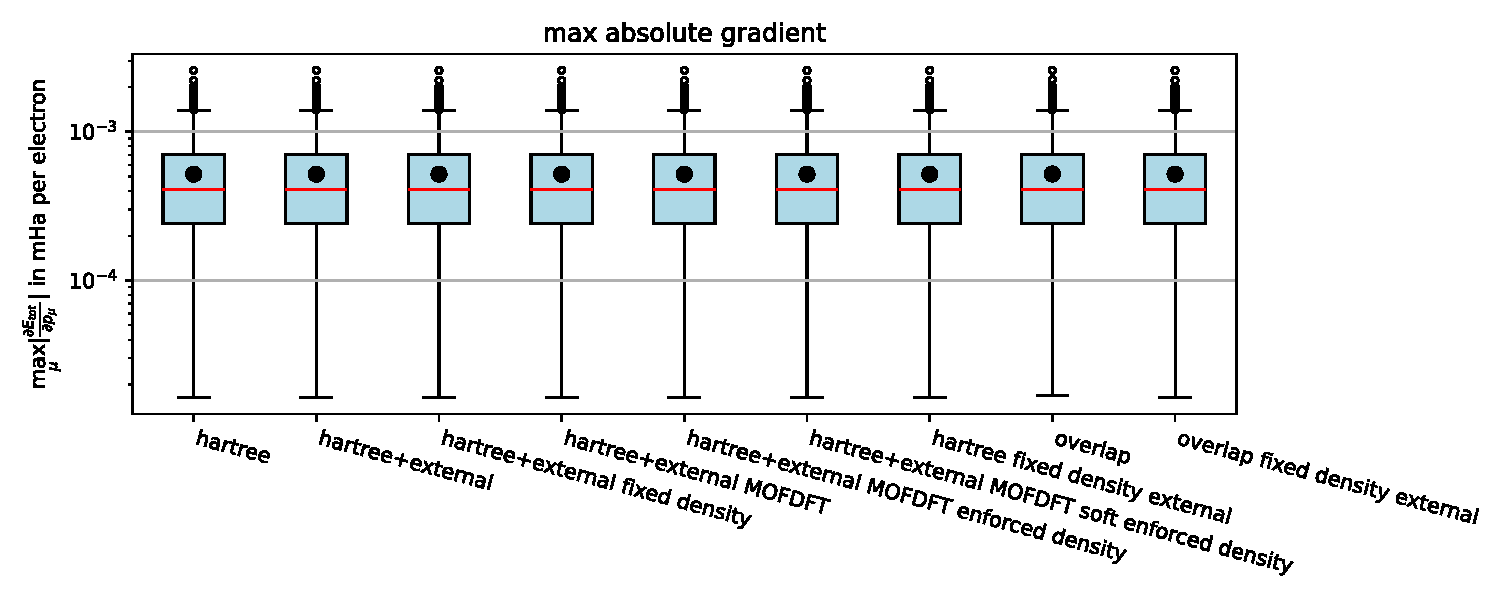
\includegraphics[width=0.49\textwidth]{chapters/results/results_images/max_abs_gradient_on_even_tempered_2.5}
    \includesvg[width=0.5\textwidth]{chapters/results/results_images/var_density_fitting}
    \caption{A plot of the different metrics evaluated on the first 1000 Molecules of the QM9 dataset}
    \label{fig:my_label}
\end{figure}

\begin{figure}[h]
    \centering
    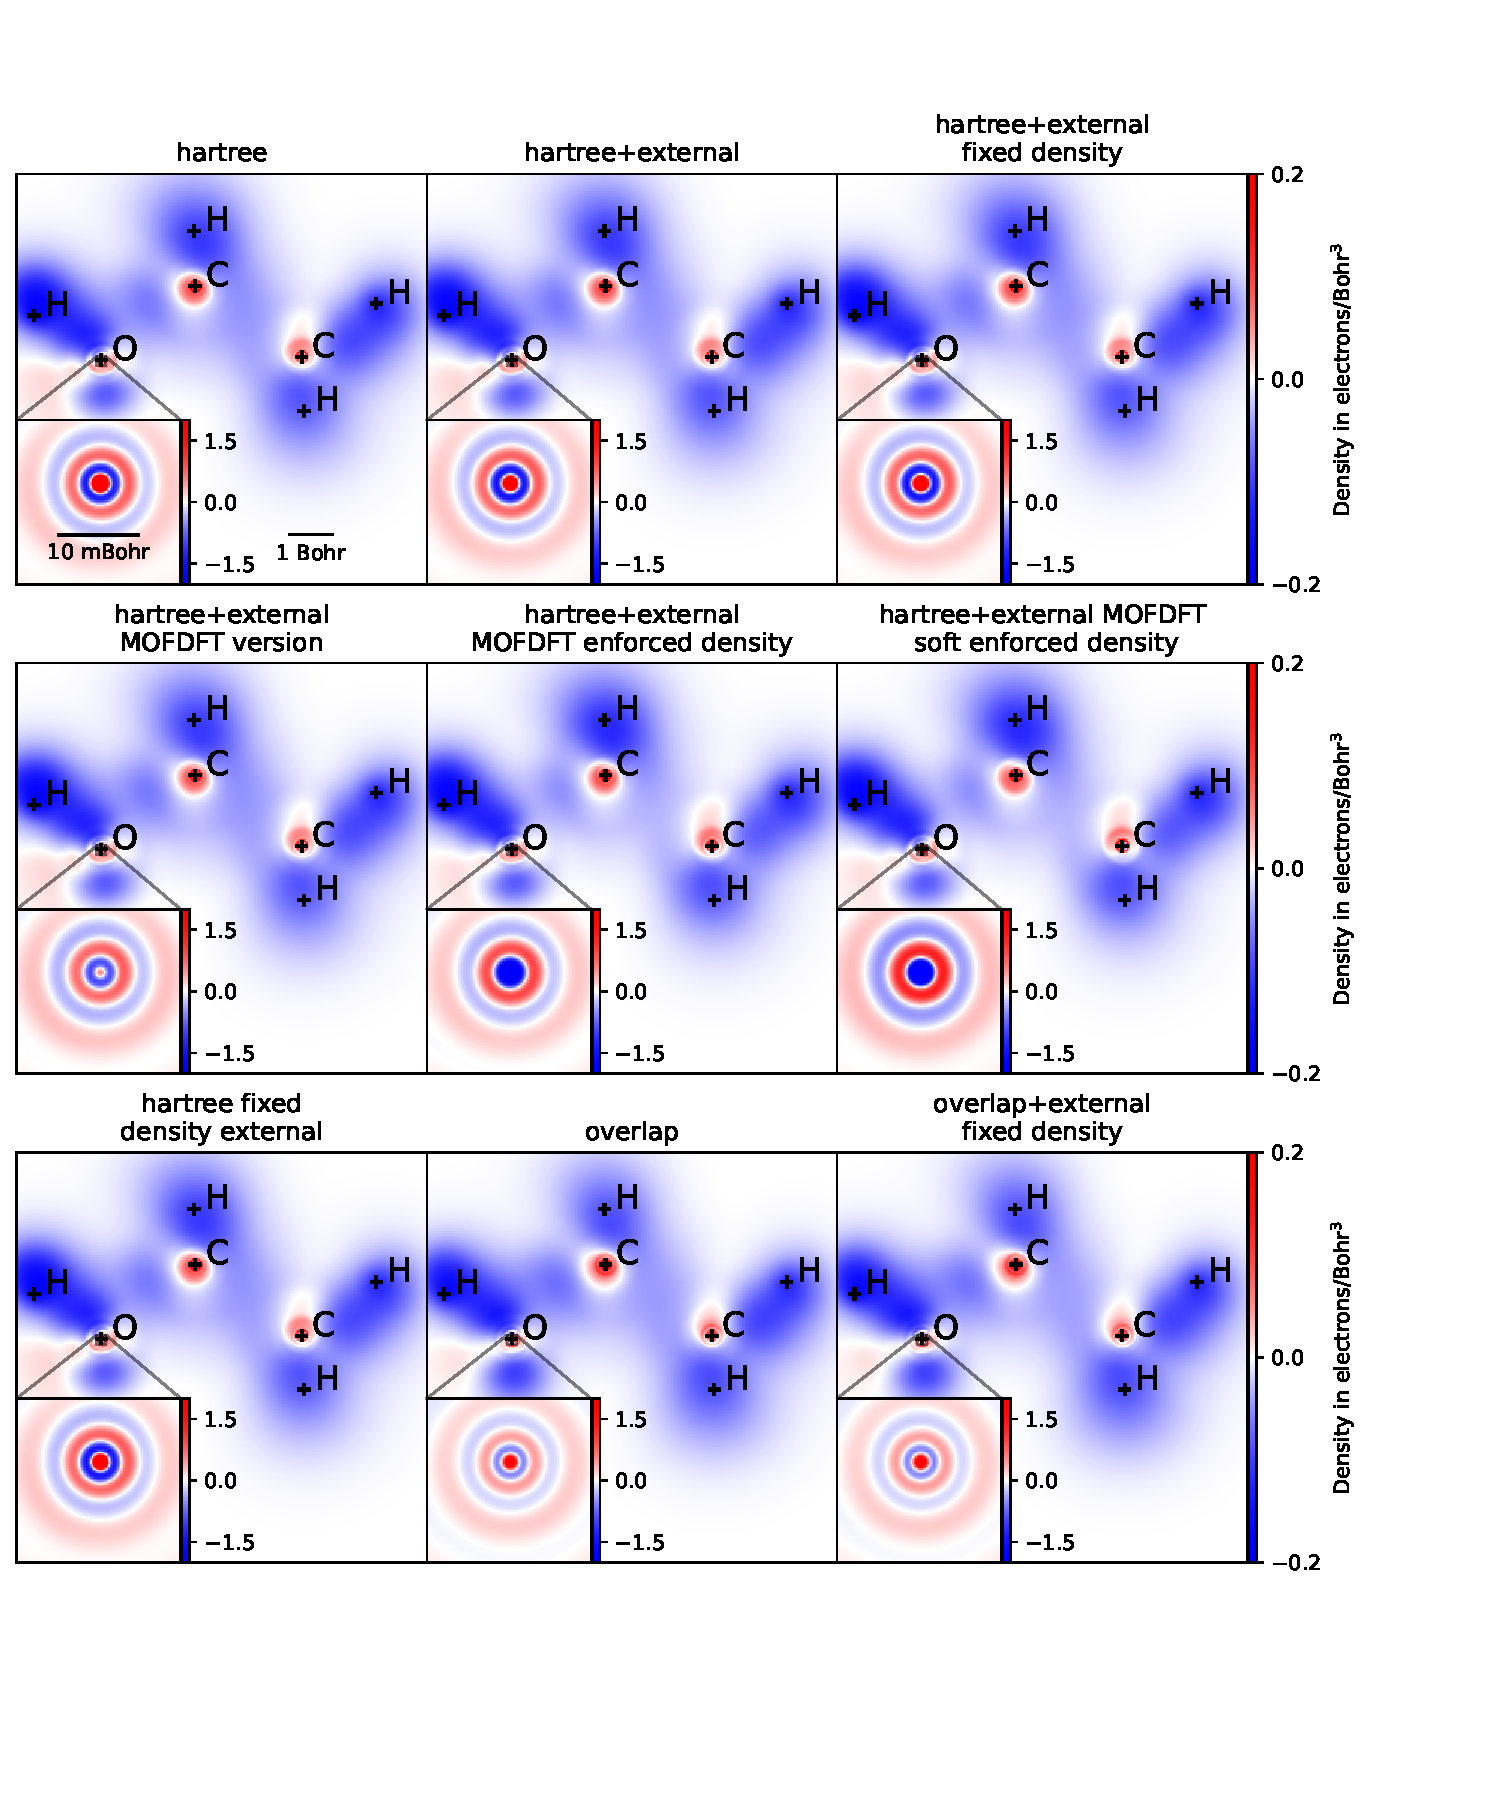
\includegraphics[width=1\textwidth]{chapters/results/results_images/density_fitting_slices}
    \caption{A plot of the different metrics evaluated on the first 1000 Molecules of the QM9 dataset}
    \label{fig:my_label2}
\end{figure}








    \chapter{Orbital Free Basis Set Fitting Tabels}
    \begin{figure}
    \centering
    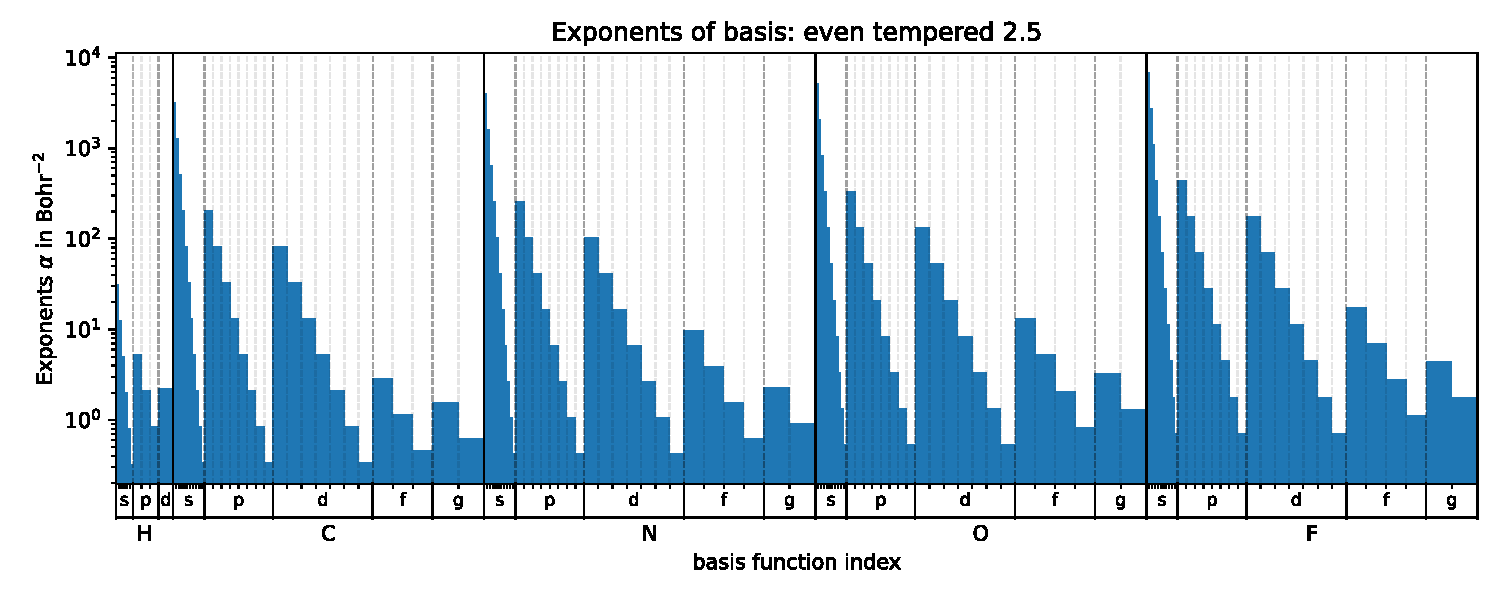
\includegraphics[width=0.49\textwidth]{chapters/results/results_images/basis_functions_even_tempered_2.5}
    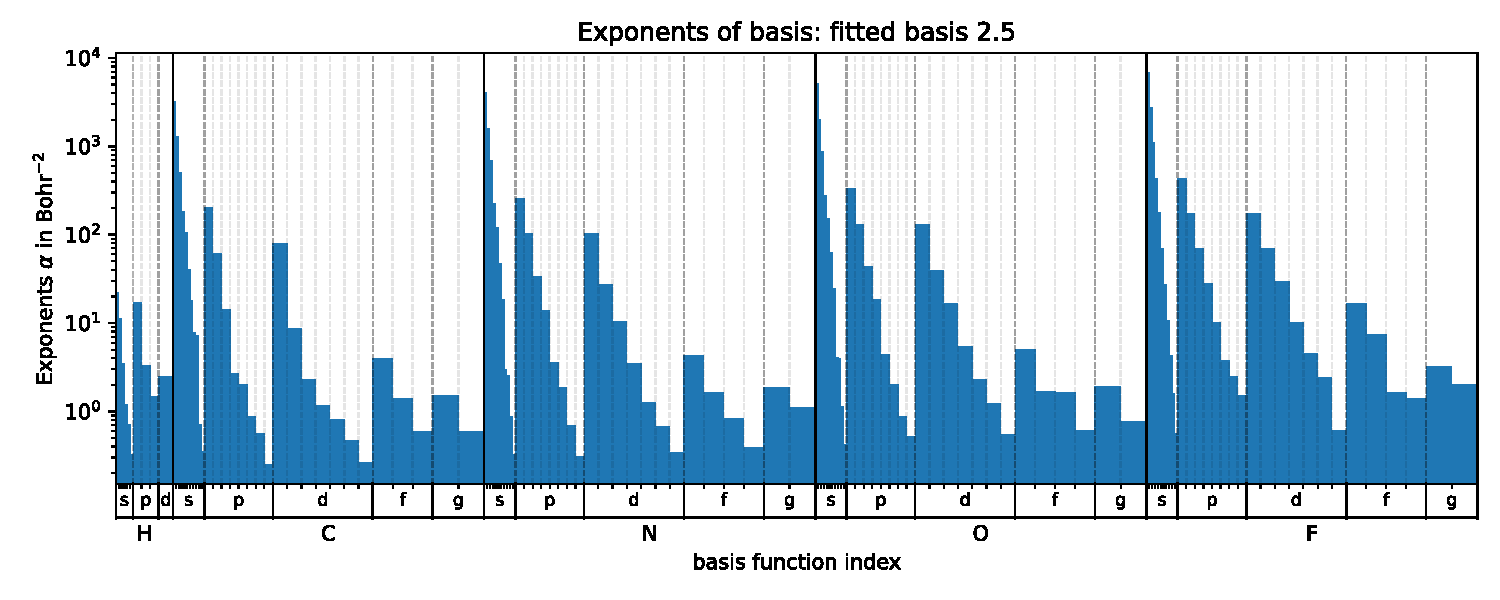
\includegraphics[width=0.5\textwidth]{chapters/results/results_images/basis_functions_fitted_basis_2.5}
    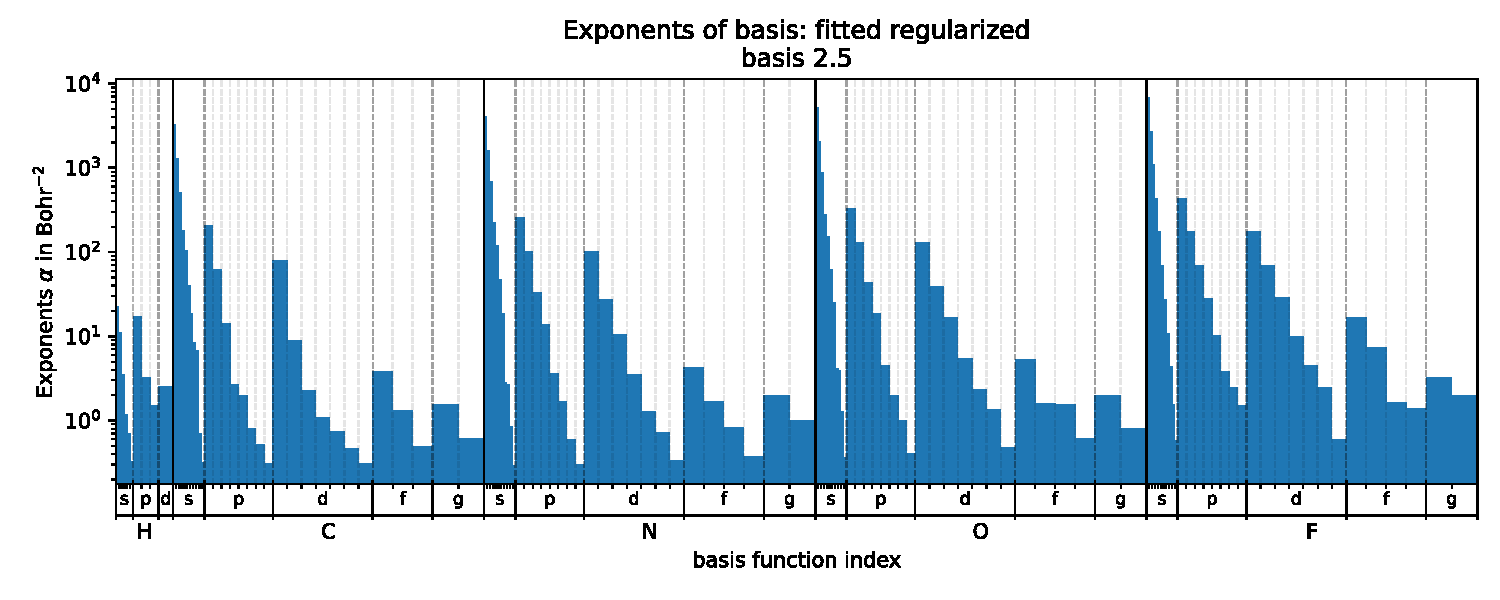
\includegraphics[width=0.49\textwidth]{chapters/results/results_images/basis_functions_fitted_regularized_basis_2.5}
    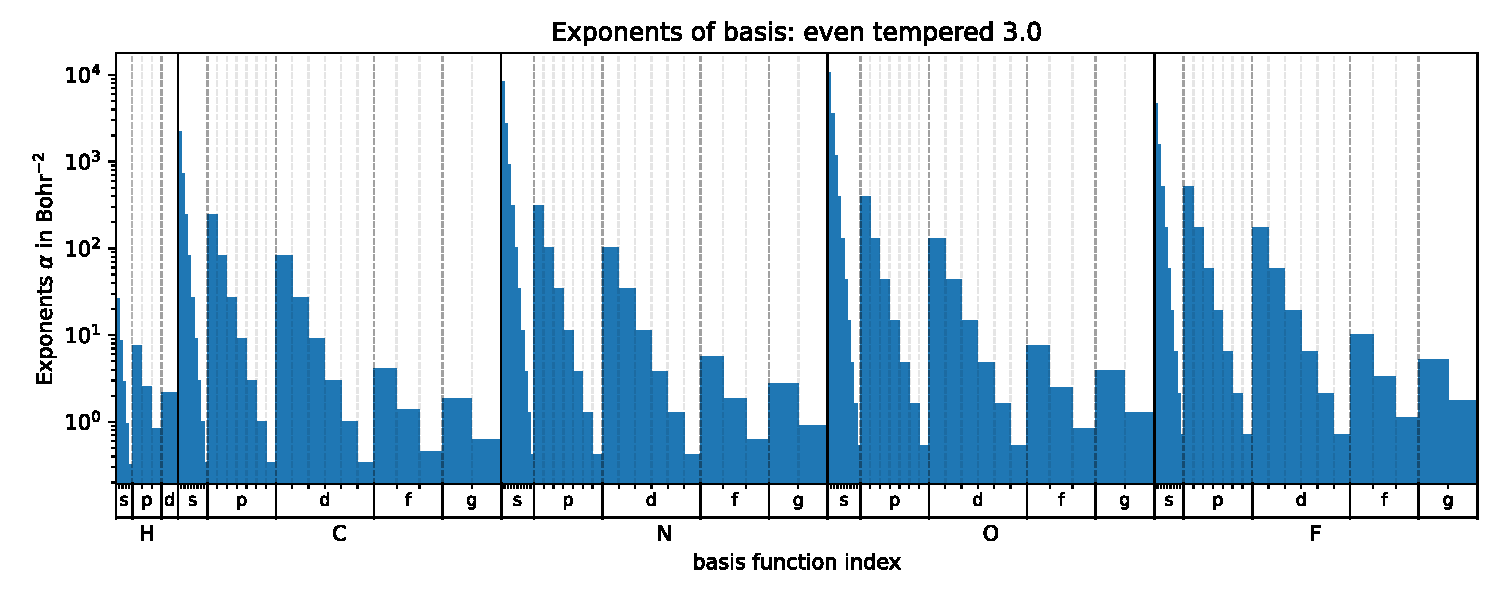
\includegraphics[width=0.5\textwidth]{chapters/results/results_images/basis_functions_even_tempered_3.0}
    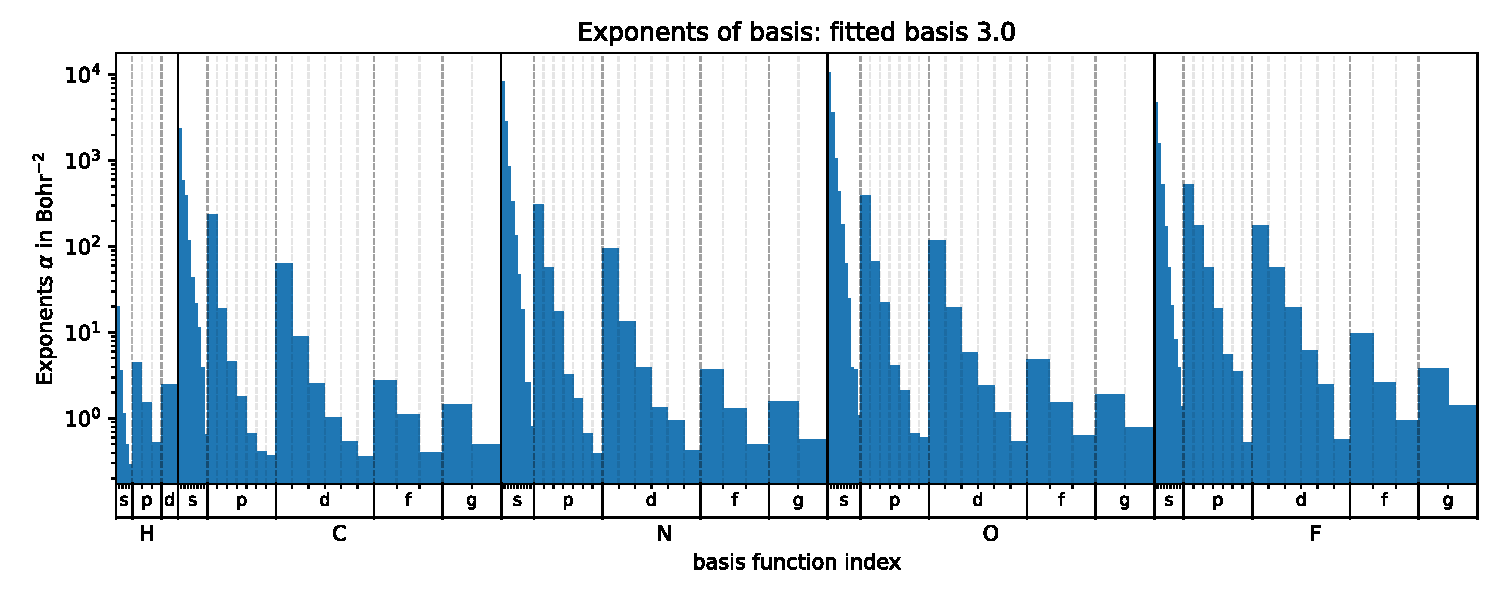
\includegraphics[width=0.49\textwidth]{chapters/results/results_images/basis_functions_fitted_basis_3.0}
    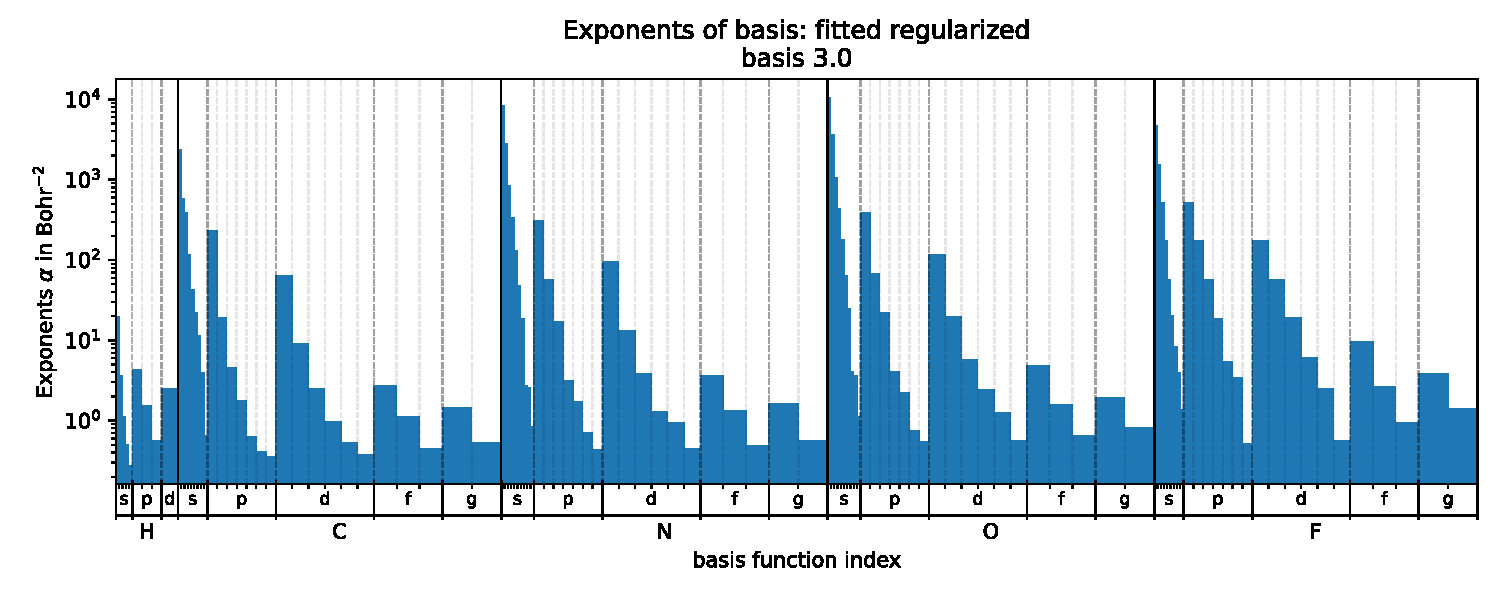
\includegraphics[width=0.5\textwidth]{chapters/results/results_images/basis_functions_fitted_regularized_basis_3.0}
    \caption{Plots comparing the basis functions of the fitted basis sets to the even tempered basis set}
\end{figure}

\begin{figure}
    \centering
        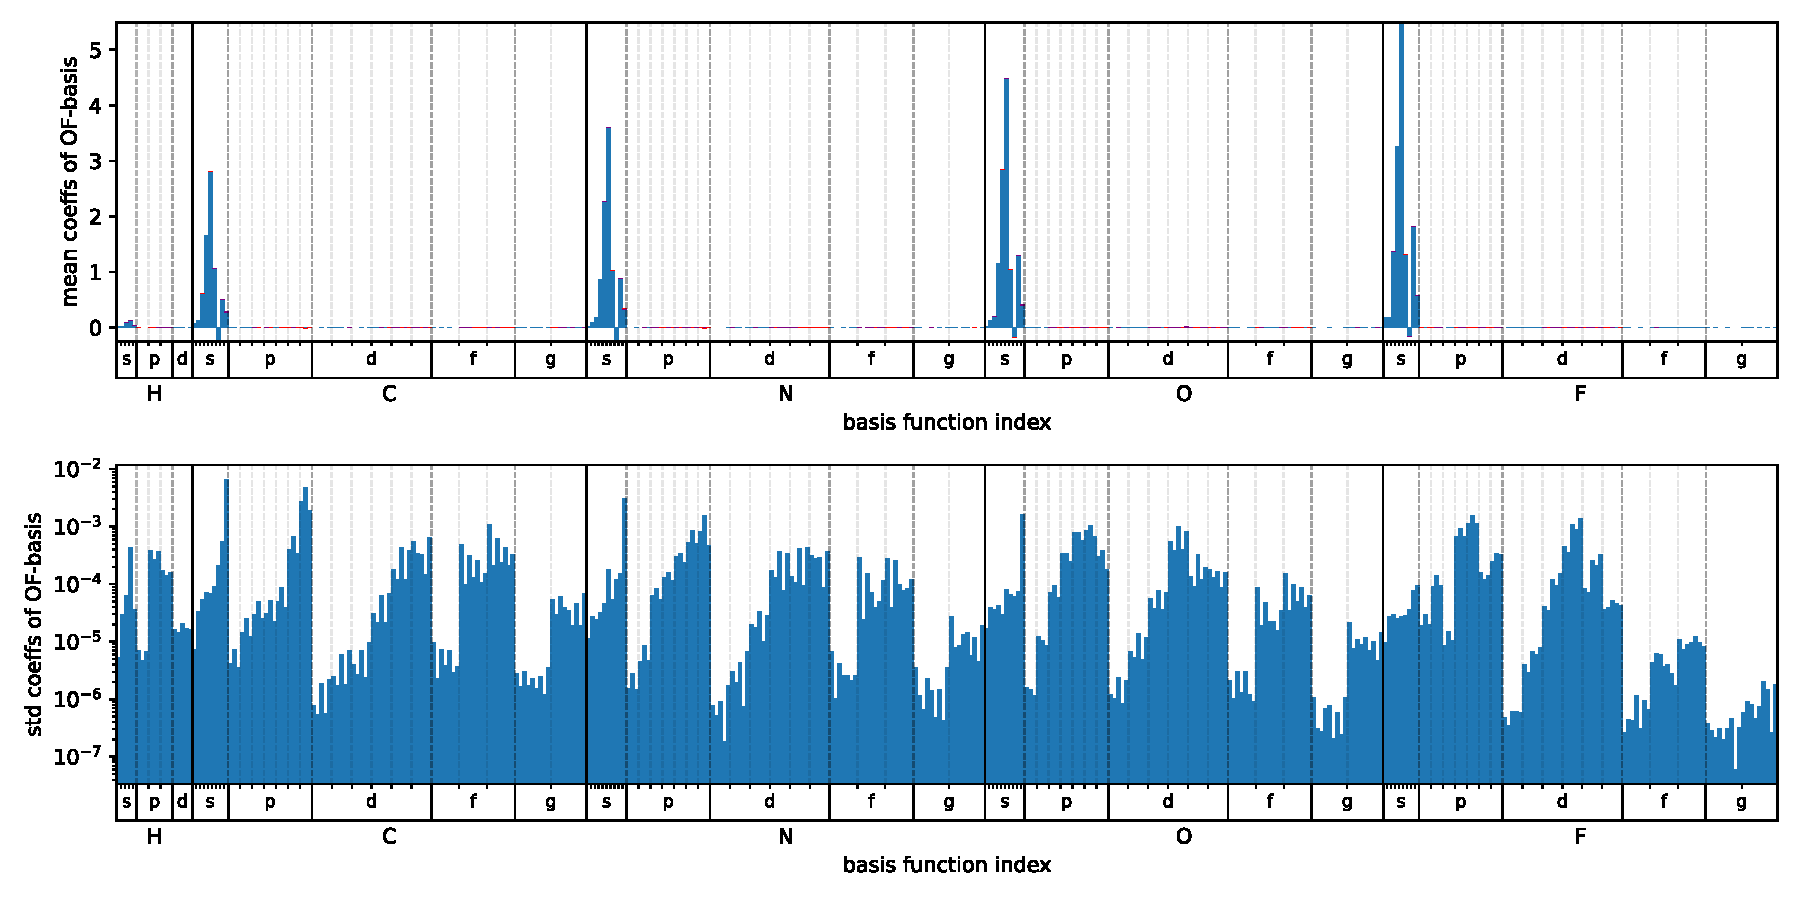
\includegraphics[width=0.49\textwidth]{chapters/results/results_images/var_coeffseven_tempered_3.0}
        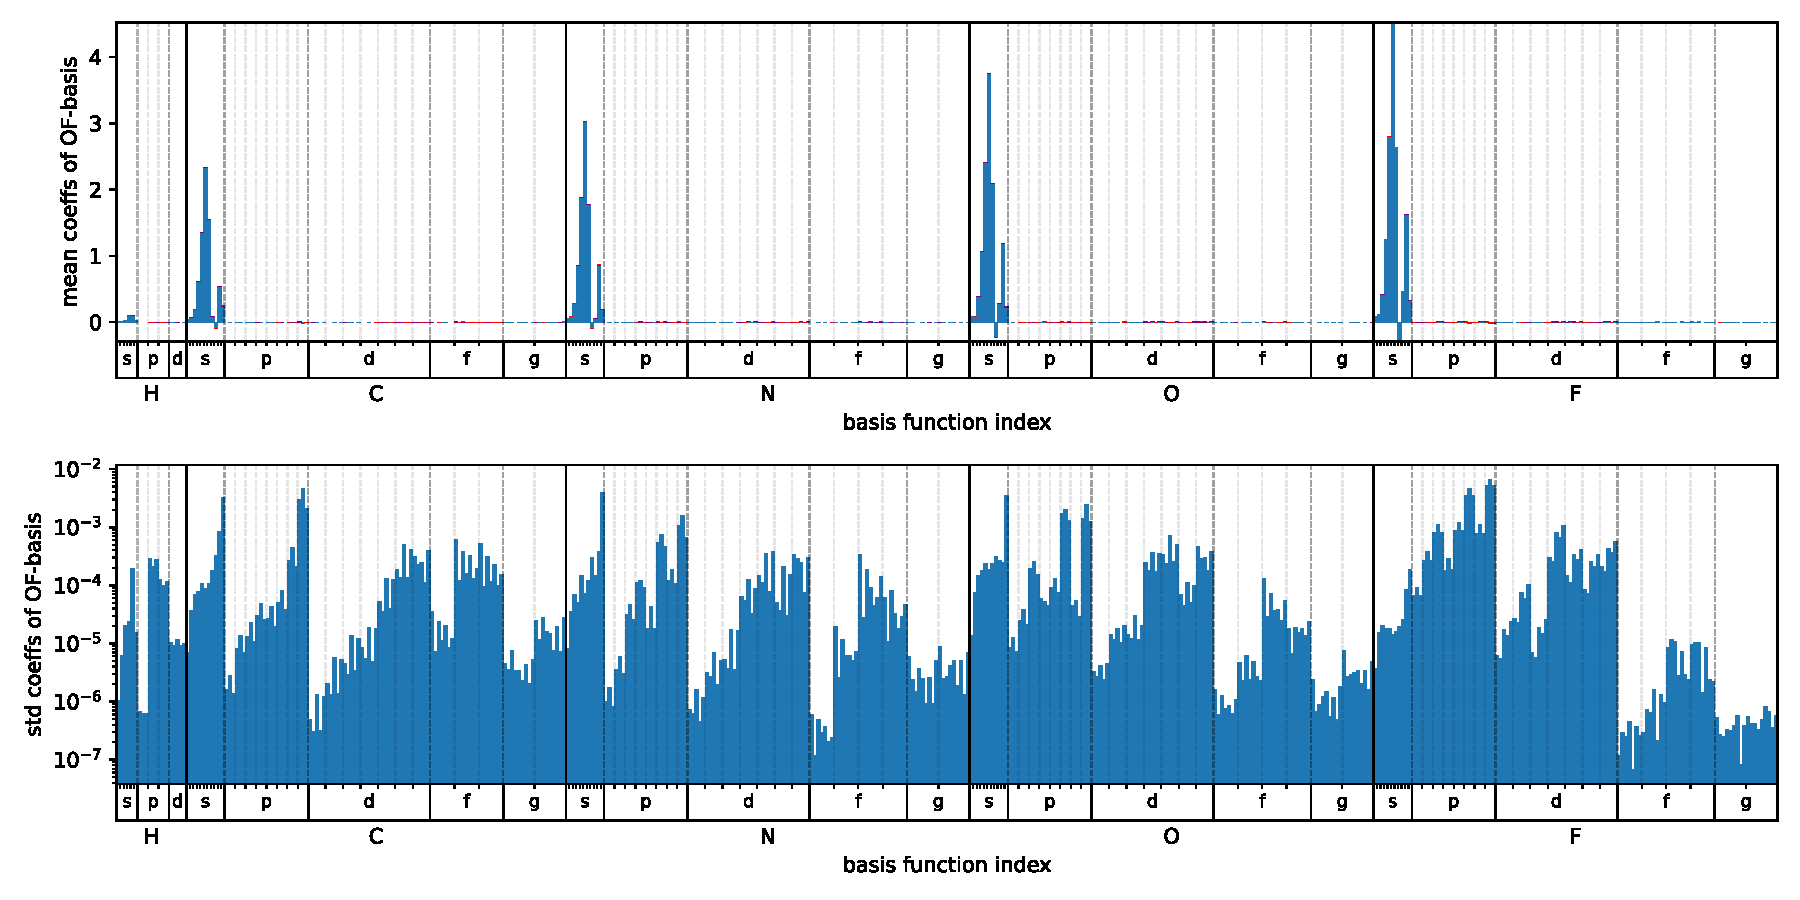
\includegraphics[width=0.5\textwidth]{chapters/results/results_images/var_coeffseven_tempered_2.5}
        \includegraphics[width=0.49\textwidth]{chapters/results/results_images/var_coeffseven_tempered_2.0}
        \includegraphics[width=0.5\textwidth]{chapters/results/results_images/var_coeffseven_tempered_1.5}
        \includegraphics[width=0.49\textwidth]{chapters/results/results_images/var_coeffsfitted_basis_3.0}
        \includegraphics[width=0.5\textwidth]{chapters/results/results_images/var_coeffsfitted_basis_2.5}
        \includegraphics[width=0.49\textwidth]{chapters/results/results_images/var_coeffsfitted_regularized_basis_3.0}
        \includegraphics[width=0.5\textwidth]{chapters/results/results_images/var_coeffsfitted_regularized_basis_2.5}
    \caption{Variance of the coefficients for the different basis sets}
\end{figure}
    \chapter{Adaptive Basis Sets Additional Material}
    \section{Derivation of the loss function}
One of the characteristics of orbitals is that they are orthonormal to each other. But if we try to fit orbitals naively we won't be able to guarantee this property. To ensure that the fitted orbitals are orthonormal we can use the following loss function wich enforces the orthogonormality of the orbitals using laplace multipliers:
\begin{align}
    \{\phi_i\}_{i=1,...,N_e} = \underset{\{\phi_i\}_{i=1,...,N_e} pairwise orthonormal}{\text{argmin}}\sum\limits_{i=1}^{N_e} \int (\phi_i(\mathbf{r})-\phi'_i(\mathbf{r}))^2 d\mathbf{r}
\end{align}
In components we can define the lagrangian as:
\begin{align}
\mathcal{L}(\{C_{i\mu}\}_{i=1,...,N_e,\mu=1,...,N_b}) &= \sum\limits_{i=1}^{N_e} \int (\phi_i(C,\mathbf{r})-\phi'_i(\mathbf{r}))^2 d\mathbf{r} + \sum\limits_{i=1}^{N_e} \sum\limits_{j=1}^{N_e} \lambda_{ij}\left( \int \phi_i(C,\mathbf{r})\phi_j(C,\mathbf{r}) d\mathbf{r}- \delta_{ij}\right)\\
    &= \sum\limits_{i=1}^{N_e} C_{i,\mu} \langle \eta_\mu|\eta_\nu \rangle C_{i,\nu} - 2 C_{i,\mu} \langle \eta_\mu|\eta'_\nu \rangle C'_{i,\nu} + C'_{i,\mu} \langle \eta'_\mu|\eta'_\nu \rangle C'_{i,\nu}\\
    &+ \sum\limits_{i=1}^{N_e} \sum\limits_{j=1}^{N_e} \lambda_{ij}\left( C_{i,\mu} \langle \eta_\mu|\eta_\nu \rangle  C_{j,\nu} - \delta_{ij}\right)
\end{align}
Where $\{\lambda_{ij}\}_{i,j=1,...,N_e}$ are lagrange multipliers.
We can now differentiate the lagrangian with respect to the coefficients $C_{i,\mu}$ to get the following equation:
\begin{align}
    \partial_{C_{k,\gamma}}\mathcal{L} &= 2\langle \eta_\gamma|\eta_\nu \rangle C_{k,\nu} - 2 \langle \eta_\gamma|\eta'_\nu \rangle C'_{k,\nu} + 2 \sum\limits_{j=1}^{N_e} \lambda_{kj} \langle \eta_\gamma|\eta_\nu \rangle  C_{j,\nu} = 0\label{deriv_eq}\\
    \partial_{\lambda_{ij}}\mathcal{L} &= C_{i,\mu} \langle \eta_\mu|\eta_\nu \rangle  C_{j,\nu} - \delta_{ij} = 0
\end{align}
Now we contract it with $C_{l,\gamma}$ and $C'_{l,\mu} \langle \eta'_\mu|\eta_\sigma \rangle\langle \eta_\cdot|\eta_\cdot \rangle^{-1}_{\sigma\gamma}$:
\begin{align}
    C_{l,\gamma}\partial_{C_{k,\gamma}}\mathcal{L} &= 2 C_{l,\gamma}\langle \eta_\gamma|\eta_\nu \rangle C_{k,\nu} - 2 C_{l,\gamma} \langle \eta_\gamma|\eta'_\nu \rangle C'_{k,\nu} + 2 \sum\limits_{j=1}^{N_e} \lambda_{kj} C_{l,\gamma}  \langle \eta_\gamma|\eta_\nu \rangle  C_{j,\nu} \\
    &= 2 \delta_{lk} - 2 C_{l,\gamma} \langle \eta_\gamma|\eta'_\nu \rangle C'_{k,\nu} + 2 \sum\limits_{j=1}^{N_e} \lambda_{kj} \delta_{lj}\\
    &=2 \delta_{lk} - 2 C_{l,\gamma} \langle \eta_\gamma|\eta'_\nu \rangle C'_{k,\nu} + 2 \lambda_{kl}= 0\\
        &\Rightarrow C_{l,\gamma} \langle \eta_\gamma|\eta'_\nu \rangle C'_{k,\nu} = \delta_{lk} + \lambda_{kl}\label{xyz}\\
    C'_{l,\mu} \langle \eta'_\mu|\eta_\sigma \rangle\langle \eta_\cdot|\eta_\cdot \rangle^{-1}_{\sigma\gamma}\partial_{C_{k,\gamma}}\mathcal{L} &= 2 C'_{l,\mu} \langle \eta'_\mu|\eta_\sigma \rangle\langle \eta_\cdot|\eta_\cdot \rangle^{-1}_{\sigma\gamma}\langle \eta_\gamma|\eta_\nu \rangle C_{k,\nu} - 2 C'_{l,\mu} \langle \eta'_\mu|\eta_\sigma \rangle\langle \eta_\cdot|\eta_\cdot \rangle^{-1}_{\sigma\gamma} \langle \eta_\gamma|\eta'_\nu \rangle C'_{k,\nu}\\
    &+ 2 \sum\limits_{j=1}^{N_e} \lambda_{kj} C'_{l,\mu} \langle \eta'_\mu|\eta_\sigma \rangle\langle \eta_\cdot|\eta_\cdot \rangle^{-1}_{\sigma\gamma} \langle \eta_\gamma|\eta_\nu \rangle  C_{j,\nu} \\
    &=2 C'_{l,\mu} \langle \eta'_\mu|\eta_\nu \rangle C_{k,\nu} - 2 C'_{l,\mu} \langle \eta'_\mu|\eta_\sigma \rangle\langle \eta_\cdot|\eta_\cdot \rangle^{-1}_{\sigma\gamma} \langle \eta_\gamma|\eta'_\nu \rangle C'_{k,\nu}\\
    &+ 2 \sum\limits_{j=1}^{N_e} \lambda_{kj} C'_{l,\mu} \langle \eta'_\mu|\eta_\nu \rangle  C_{j,\nu} =0\label{last}
    \end{align}
Now insert \eqref{xyz} into \eqref{last}:
\begin{align}
    0&=\delta_{lk} + \lambda_{kl} - C'_{l,\mu} \langle \eta'_\mu|\eta_\sigma \rangle\langle \eta_\cdot|\eta_\cdot \rangle^{-1}_{\sigma\gamma} \langle \eta_\gamma|\eta'_\nu \rangle C'_{k,\nu} + \sum\limits_{j=1}^{N_e} \lambda_{kj} \left(\delta_{lj} + \lambda_{lj}\right) \\
    &= \sum\limits_{j=1}^{N_e} \lambda_{kj}\lambda_{jl} +2\lambda_{kl} - C'_{l,\mu} \langle \eta'_\mu|\eta_\sigma \rangle\langle \eta_\cdot|\eta_\cdot \rangle^{-1}_{\sigma\gamma} \langle \eta_\gamma|\eta'_\nu \rangle C'_{k,\nu} + \delta_{lk}
\end{align}
This is just a quadratic matrix equation which can be solved for $\lambda_{kl}$.\\
We now define
\begin{equation}
    A_{ij}:= C'_{i,\mu} \langle \eta'_\mu|\eta_\sigma \rangle\langle \eta_\cdot|\eta_\cdot \rangle^{-1}_{\sigma\gamma} \langle \eta_\gamma|\eta'_\nu \rangle C'_{j,\nu}
\end{equation}
\begin{align}
    \lambda_{lk,\pm} = \delta_{lk} \pm \sqrt{\delta_{lk}+A_{lk}-\delta_{lk}} = \delta_{lk} \pm \sqrt{A_{lk}}
\end{align}
Now we can insert the lagrange multipliers back into \eqref{deriv_eq} and invert it:
\begin{align}
   0&=\langle \eta_\gamma|\eta_\nu \rangle C_{k,\nu} - \langle \eta_\gamma|\eta'_\nu \rangle C'_{k,\nu} + \sum\limits_{j=1}^{N_e} \left(\delta_{kj} \pm \sqrt{A_{kj}}\right) \langle \eta_\gamma|\eta_\nu \rangle  C_{j,\nu}\\
    &= - \langle \eta_\gamma|\eta'_\nu \rangle C'_{k,\nu} + \sum\limits_{j=1}^{N_e} \left(\delta_{kj}+\left(- \delta_{kj} \pm \sqrt{A_{kj}}\right)\right) \langle \eta_\gamma|\eta_\nu \rangle  C_{j,\nu}\\
    &= - \langle \eta_\gamma|\eta'_\nu \rangle C'_{k,\nu} + \sum\limits_{j=1}^{N_e} \left(\pm \sqrt{A_{kj}}\right) \langle \eta_\gamma|\eta_\nu \rangle  C_{j,\nu}\\
    C_{j,\nu}&= \sum\limits_{k=1}^{N_e}  A^{-\frac{1}{2}}_{kj} \langle \eta_\gamma|\eta_\nu \rangle^{-1} \langle \eta_\gamma|\eta'_\nu \rangle C'_{k,\nu}
\end{align}





\end{appendices}
\printbibliography[heading=bibintoc, title={Complete bibliography}]
%Displays the whole bibliography with the title "Complete bibliography"                  
\clearpage
%Filtering bibliography
\newpage
%\includepdf[pages=1]{images/Selbststaendigkeitserklaerung.pdf}

\end{document}